\documentclass[supercite]{Experimental_Report}

\title{~~~~~~数据结构实验~~~~~~}
\author{吕博文}
\school{计算机科学与技术学院}
\classnum{CS2209}
\stunum{U202217357}
\instructor{周全}
\date{2023年6月1日}

\usepackage{algorithm, multirow}
\usepackage{algpseudocode}
\usepackage{amsmath}
\usepackage{amsthm}
\usepackage{framed}
\usepackage{mathtools}
\usepackage{subcaption}
\usepackage{xltxtra} %提供了针对XeTeX的改进并且加入了XeTeX的LOGO, 自动调用xunicode宏包(提供Unicode字符宏)
\usepackage{bm}
\usepackage{tikz}
\usepackage{tikzscale}
\usepackage{pgfplots}
%\usepackage{enumerate}
%代码
\usepackage{caption}
%\usepackage[dvipsnames]{xcolor}  % 更全的色系
\usepackage{listings}  % 排代码用的宏包
\lstset{
    language = C,
%    backgroundcolor = \color{white},    % 背景色
    basicstyle = \small\ttfamily,           % 基本样式 + 小号字体
    rulesepcolor= \color{gray},             % 代码块边框颜色
    breaklines = true,                  % 代码过长则换行
    numbers = left,                     % 行号在左侧显示
    numberstyle = \small,               % 行号字体
    keywordstyle = \color{blue}\bfseries,      % 关键字颜色
    commentstyle =\bfseries\color{teal},        % 注释颜色
    stringstyle = \color{purple},          % 字符串颜色
%    frame = shadowbox,                  % 用(带影子效果)方框框住代码块
	frame=single,
    showspaces = false,                 % 不显示空格
    columns = fixed,                    % 字间距固定
    %escapeinside={<@}{@>}              % 特殊自定分隔符:<@可以自己加颜色@>
    morekeywords = {status,ElemType,LISTINCREMENT,SqList,TElemType,BiTree,KeyType,QElemType},                % 自加新的关键字(必须前后都是空格)
    deletendkeywords = {compile}        % 删除内定关键字;删除错误标记的关键字用deletekeywords删!
}

\pgfplotsset{compat=1.16}

\newcommand{\cfig}[3]{
  \begin{figure}[htb]
    \centering
    \includegraphics[width=#2\textwidth]{images/#1.tikz}
    \caption{#3}
    \label{fig:#1}
  \end{figure}
}

\newcommand{\sfig}[3]{
  \begin{subfigure}[b]{#2\textwidth}
    \includegraphics[width=\textwidth]{images/#1.tikz}
    \caption{#3}
    \label{fig:#1}
  \end{subfigure}
}

\newcommand{\xfig}[3]{
  \begin{figure}[htb]
    \centering
    #3
    \caption{#2}
    \label{fig:#1}
  \end{figure}
}

\newcommand{\rfig}[1]{\autoref{fig:#1}}
\newcommand{\ralg}[1]{\autoref{alg:#1}}
\newcommand{\rthm}[1]{\autoref{thm:#1}}
\newcommand{\rlem}[1]{\autoref{lem:#1}}
\newcommand{\reqn}[1]{\autoref{eqn:#1}}
\newcommand{\rtbl}[1]{\autoref{tbl:#1}}

\algnewcommand\Null{\textsc{null }}
\algnewcommand\algorithmicinput{\textbf{Input:}}
\algnewcommand\Input{\item[\algorithmicinput]}
\algnewcommand\algorithmicoutput{\textbf{Output:}}
\algnewcommand\Output{\item[\algorithmicoutput]}
\algnewcommand\algorithmicbreak{\textbf{break}}
\algnewcommand\Break{\algorithmicbreak}
\algnewcommand\algorithmiccontinue{\textbf{continue}}
\algnewcommand\Continue{\algorithmiccontinue}
\algnewcommand{\LeftCom}[1]{\State $\triangleright$ #1}

\newtheorem{thm}{定理}[section]
\newtheorem{lem}{引理}[section]

\colorlet{shadecolor}{black!15}

\theoremstyle{definition}
\newtheorem{alg}{算法}[section]

\def\thmautorefname~#1\null{定理~#1~\null}
\def\lemautorefname~#1\null{引理~#1~\null}
\def\algautorefname~#1\null{算法~#1~\null}

\begin{document}

\maketitle


\clearpage

\pagenumbering{Roman}

\tableofcontents[level=2]

\clearpage

\pagenumbering{arabic}

\section{基于链式存储结构的线性表实现}


\subsection{问题描述}

本实验实现了线性表的链式存储,构造一个具有菜单功能的演示系统,实现了线性表的初始化、销毁、清空等基本功能和全部的5种附加功能,并实现了多线性表管理。

\subsection{系统设计}

链表作为一种线性结构,在数据结构中应用广泛,是最常用、最基本的结构类型之一。本次实验采用链表的线性存储方式,实现了链表基本的功能,比如增添、删除、遍历等。同时,还在此基础上添加了一些高级功能,比如翻转、倒序删除、排序等,更好地方便使用者对链表进行操作。该程序还使用语言文字提示,降低了程序的使用难度。

本实验涉及的头文件以及相关常量定义如下:
\lstset{ 
	commentstyle=\color[RGB]{0,100,0}
}
\begin{lstlisting}[title = 相关常量定义]
/* 相关头文件 */
#include <stdio.h>
#include <malloc.h>
#include <stdlib.h>

/*---------相关的常量及定义 ---------*/
#define TRUE 1//定义真值 
#define FALSE 0//定制假值 
#define OK 1//程序正常运行 
#define ERROR 0//程序运行出错 
#define INFEASTABLE -1  //没有实现的操作返回该标记
#define OVERFLOW -2  //数值溢出 
#define MAX_NUM 10   //可管理线性表的数量
#define LIST_INIT_SIZE 100  //线性表的初始存储空间大小
#define LISTINCREMENT  10  //线性表存储空间不足时增加的存储空间量
FILE *fp;  //文件指针,用于数据存储和读取
\end{lstlisting}

本系统的数据结构有两种:链式线性表和链式线性表的管理表。其具体定义如下。

\begin{lstlisting}[title = 相关数据结构定义]
typedef int status; //定义所有状态码和返回值的类型为int
typedef int ElemType; //数据元素类型定义
typedef struct LNode{  //定义单链表节点结构体类型
	ElemType data;  //节点中存储的数据元素
	struct LNode *next;  //指向下一个节点的指针
}LNode, *LinkList;

\end{lstlisting}


系统的总体架构:界面上采用简易菜单演示系统,在 while 循环中建立菜单
演示,op 代表用户选择的操作序号,程序将首先判断 op 的合法性,若合法则通
过 switch 函数进入功能的选择,进入相关功能函数执行相关操作,操作完成后
继续执行循环,直到用户输入 0 时,退出系统。

多线性表管理通过ChooseList函数实现,用户可以输入位序切换线性表,相关操作仅在当前线性表完成,而不会影响线性表组。
\begin{figure}[H]
	\centering
	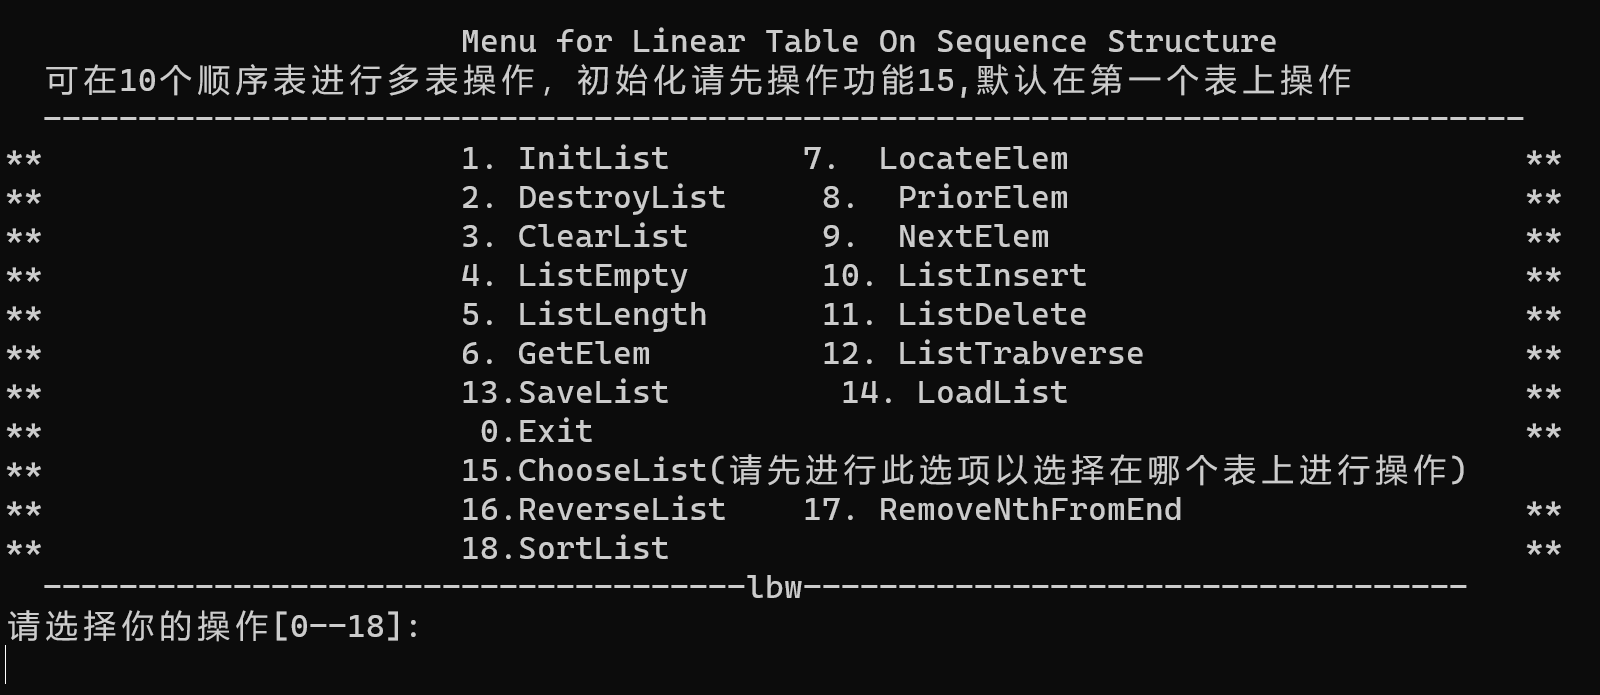
\includegraphics[width=1\linewidth]{images/菜单设计.png}
	\caption{菜单演示系统}
	\label{fig1-1}
\end{figure}
\subsection{系统实现}
本程序在 Windows 11 系统下采用 Dev-C++ 进行编译调试,语言选择 C 语言
以下主要说明各个主要函数的实现思想,函数和系统实现的源代码放在附录中。

(\emph{本实验所有函数在实现功能之前会先对是否已有线性表进行判定,若无线性
表,则返回 INFEASIBLE,在各函数具体设计思路中不再叙述此条。})

\begin{enumerate}
	\item 初始化线性表\\
	函数名称是 InitList(L),初始条件是线性表不存在。操作结果是构造一个空的线性表。
	
	在设计链表结构体时,需要添加一个名为 next 的结构体指针,以实现链表结构体单元之间的关联。然而,该指针是初始化时未被赋值的,因此链表的初始化是一个重要步骤。为了给结构体指针赋值,需要使用 malloc 函数,它可以分配固定空间大小的地址。初始化链表时,我们需要创建一个头结点,这个头结点的 next 指针需要赋空值,以确保程序的稳定性。
	
	\emph{复杂度:时间复杂度 T(n) = O(1)}
	\item 销毁线性表\\
	函数名称是DestroyList(L),初始条件是线性表L已存在,操作结果是销毁线性表L。
	
	在销毁链表时,不能直接清空头结点作为销毁,否则会导致程序内存泄漏,最终可能导致内存溢出和程序崩溃。正确的做法是使用 free() 函数释放每个结点的内存,并在清空所有结点后将头指针 L 赋值为空。这种做法能够及时释放占用的内存空间,使程序占用的空间保持稳定,有效提高程序的稳定性。清空过程可采用 while 循环遍历结点,并在出现空指针时结束循环,保证每个结点都得到了清空。
	
	\emph{复杂度:时间复杂度 T(n) = O(1)}
	\item 清空线性表\\
	函数名称是ClearList(L),初始条件是线性表L已存在,操作结果是将L重置为空表。
	
	该函数与销毁表函数唯一的区别在于是否考虑头结点。销毁表意味着整个链表都会彻底消失,而清空链表则是将链表中的所有数据清空,但链表本身仍然存在。因此,在清空链表之前必须确保链表的头结点存在。因此,该函数从头结点的下一个节点开始循环删除链表的所有节点,并将头结点的下一个节点赋值为空,以确保链表清空且仍然可用。
	
	\emph{复杂度:时间复杂度 T(n) = O(1)}
	\item 判定线性表是否为空\\
	判定空表:函数名称是ListEmpty(L);初始条件是线性表L已存在;操作结果是若L为空表则返回TRUE,否则返回FALSE;
	
	简而言之,空表表示头结点存在但没有任何子节点。因此,当我们清空链表时,我们需要确定链表是否为空,这可以通过检查头结点的 next 指针是否为空来实现。如果链表为空,则不需要进行清空操作。否则,我们将从头结点的下一个节点开始循环删除链表的所有节点,并将头结点的 next 指针赋值为空,以确保链表为空且仍然可用。值得注意的是,如果我们直接将头结点赋值为空,那么整个链表将无法访问并最终导致内存泄漏。
	
	\emph{复杂度:时间复杂度 T(n) = O(1)}
	\item 求线性表的长度\\
	求表长:函数名称是ListLength(L);初始条件是线性表已存在;操作结果是返回L中数据元素的个数;
	
	判断链表的长度需要对链表进行一次遍历,每次遇到一个节点就将计数器加1。当遍历到链表的末尾时,计数器的值就是链表的长度。
	
	\emph{复杂度:时间复杂度 T(n) = O(1)}
	\item 获取元素\\
函数名称是GetElem(L,i,e);初始条件是线性表已存在,1≤i≤ListLength(L);操作结果是用e返回L中第i个数据元素的值;

由于i的数值范围已设置,因此可以直接处理链表数据。引入一个int变量count,用于记录当前遍历的链表位置,在count等于i时跳出循环。

为判断目标元素是否存在,我们设立了如下的判断条件:在循环结束后检查结构体指针是否为空值,若为空,则说明while循环遍历到链表尾部仍未找到目标元素,因此返回ERROR。若不为空,则说明找到了目标元素,我们将目标元素的值赋给e,并返回OK,从而实现对该需求的满足。

\emph{复杂度:时间复杂度 T(n) = O(1)}
	\item 查找元素\\
	函数名称是LocateElem(L,e,compare());初始条件是线性表已存在;操作结果是返回L中第1个与e满足关系compare()关系的数据元素的位序,若这样
	的数据元素不存在,则返回值为0。
	
	如果线性表不存在,返回不可行。遍历线性表,记录遍历到的位置,如果遍历到的节点元素是要查找的位置,返回这个位置。
	如果遍历完成后依然未找到,返回不存在。
	
	\emph{复杂度:时间复杂度 T(n) = O(n)}
	\item 获取前驱元素\\
	函数名称是PriorElem(L,cur\_e,pre\_e);初始条件是线性表L已存在;操作结果是若cur\_e是L的数据元素,且不是第一个,则用pre\_e返回它的前驱,否
	则操作失败,pre\_e无定义。
	
	如果线性表不存在,返回不可行。从第一个元素开始遍历,如果遍历到的节点元素的next是要查找的元素,返回next所指元素。
	如果遍历完成后依然未找到,返回不存在。
	
	\emph{复杂度:时间复杂度 T(n) = O(n)}
	\item  获取后继元素\\
	获得后继:函数名称是NextElem(L,cur\_e,next\_e);初始条件是线性表L已存在;操作结果是若cur\_e是L的数据元素,且不是最后一个,则用next\_e返回它的后继,
	否则操作失败,next\_e无定义。
	
	如果线性表不存在,返回不可行。遍历线性表如果遍历到的节点元素是要查找的元素且元素的next存在,返回next所指元素。
	否则返回不存在。如果遍历完成后依然未找到,返回不存在。
	
	\emph{复杂度:时间复杂度 T(n) = O(n)}
	\item 插入元素\\
	函数名称是ListInsert(L,i,e);初始条件是线性表L已存在,1≤i≤ListLength(L)+1;操作结果是在L的第i个位置之前插入新的数据元素e。
	
	如果线性表不存在,返回不可行。首先遍历链表寻找插入位置,如果索引不大于0,返回索引错误,如果遍历完成后依然未找到,返回索引错误。
	否则分配空间并插入节点。
	
	\emph{复杂度:时间复杂度 T(n) = O(n)}
	\item 删除元素\\
	函数名称是ListDelete(L,i,e);初始条件是链表L已存在且非空,1≤i≤ListLength(L);操作结果:删除L的第i个数据元素,用e返回其值。
	
	如果线性表不存在,返回不可行。首先遍历链表寻找删除位置,如果索引不大于0,返回索引错误,如果遍历完成后依然未找到,返回索引错误。
	否则删除节点。
	
	\emph{复杂度:时间复杂度 T(n) = O(n)}
	\item 遍历线性表\\
	函数名称是ListTraverse(L,visit()),初始条件是链表L已存在;操作结果是依次对L的每个数据元素调用函数visit()。
	
	如果线性表不存在,返回不可行。否则从第一个元素开始依次访问节点元素直到节点的next指向NULL。
	
	\emph{复杂度:时间复杂度 T(n) = O(n)}
	\item 翻转线性表\\
	链表翻转:函数名称是reverseList(L),初始条件是线性表L已存在,操作结果是将L翻转。
	
	我们可以通过遍历链表,逐个改变节点之间的指针关系,实现了链表的翻转。在遍历过程中,通过使用三个指针变量,即前一个节点、当前节点和下一个节点,实现了节点指针的调整,使得链表的方向被逆序。最后,将链表的头节点指向翻转后的最后一个节点,完成了链表的翻转操作。
	
	\emph{复杂度:时间复杂度 T(n) = O(n)}
%\begin{figure}[htb!]
%	\centering
%	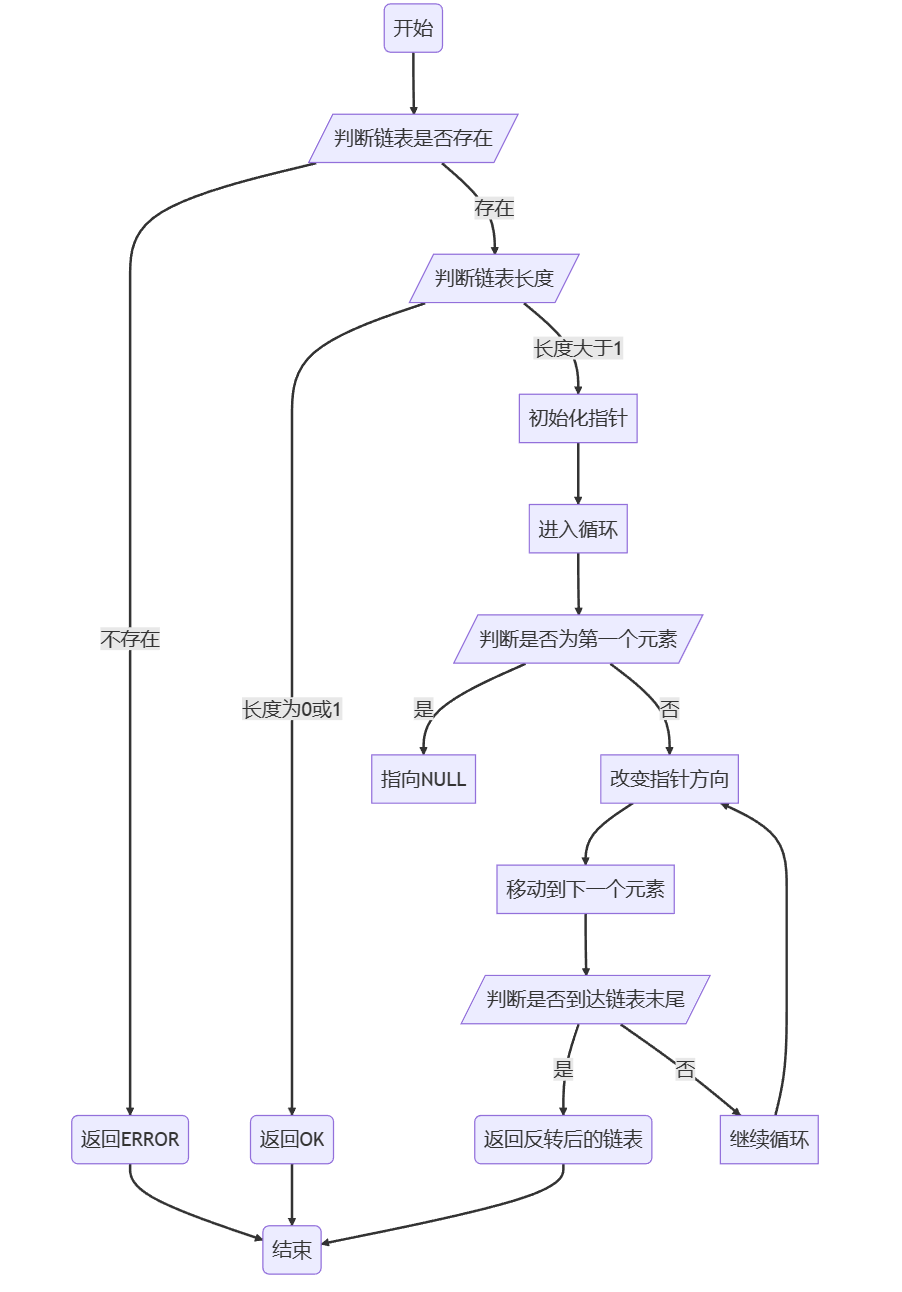
\includegraphics[width=\textwidth]{images/翻转表.png}
%	\caption{翻转线性表}
%	\label{fig1-1}
%\end{figure}
\begin{figure}[htb]
	\centering
	\begin{minipage}{0.7\linewidth}
		\centering
		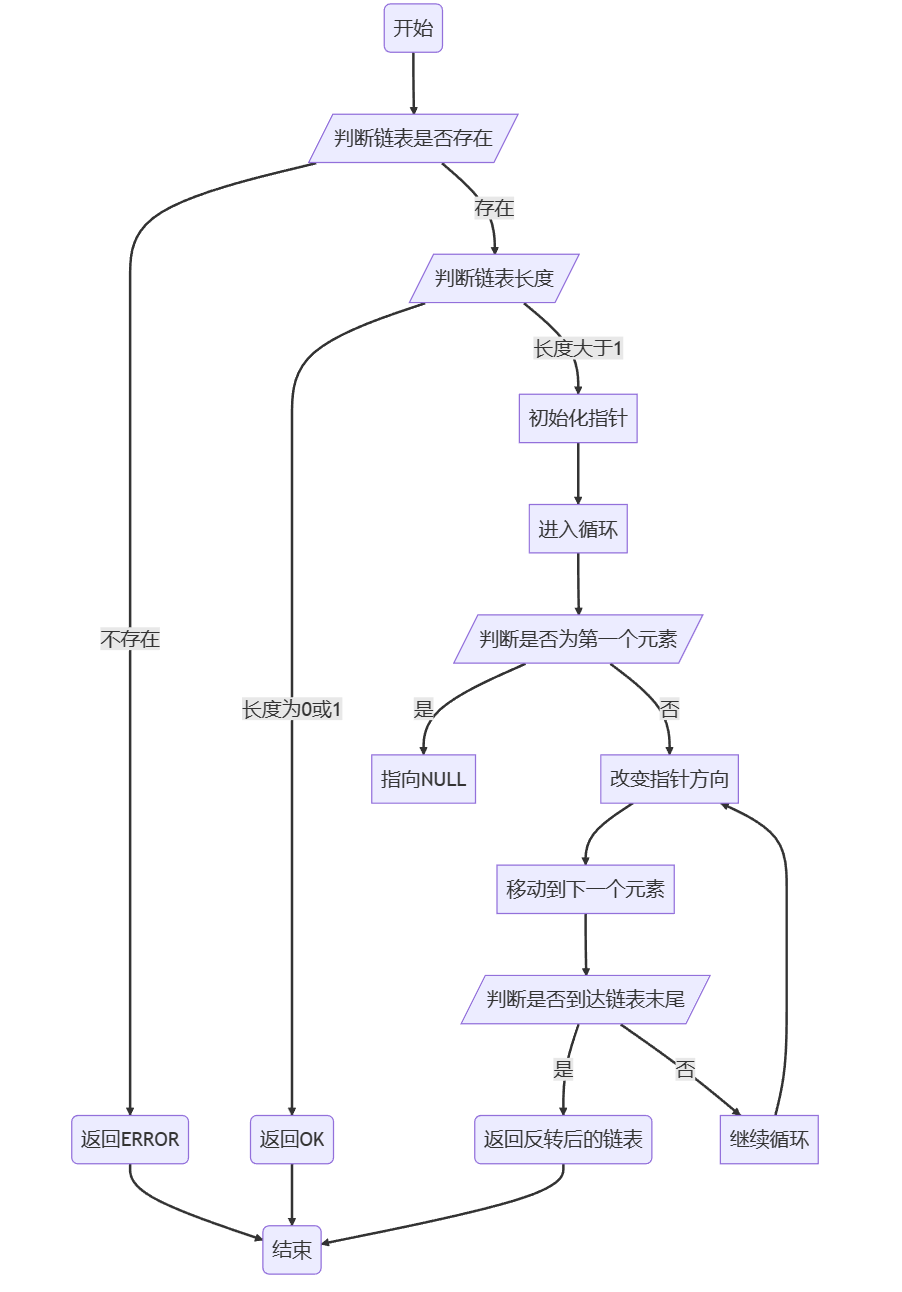
\includegraphics[width=0.9\linewidth]{images/翻转表.png}
	\end{minipage}
\caption{翻转线性表}
\label{fig1-2}
\end{figure}
	\newpage	
	\item 排序线性表\\
	函数名称是sortList(L),初始条件是线性表L已存在;操作结果是将L由小到大排序;
	
	如果线性表不存在,返回不可行。采用归并排序进行链表的排序,首先递归地从链表的中间节点拆分链表到单一节点,
	之后进行合并有序链表的操作。所有操作结束后即得到有序线性表。
	
	\emph{复杂度:时间复杂度 T(n) = O(n)}
%\begin{figure}[h]
%	\centering
%	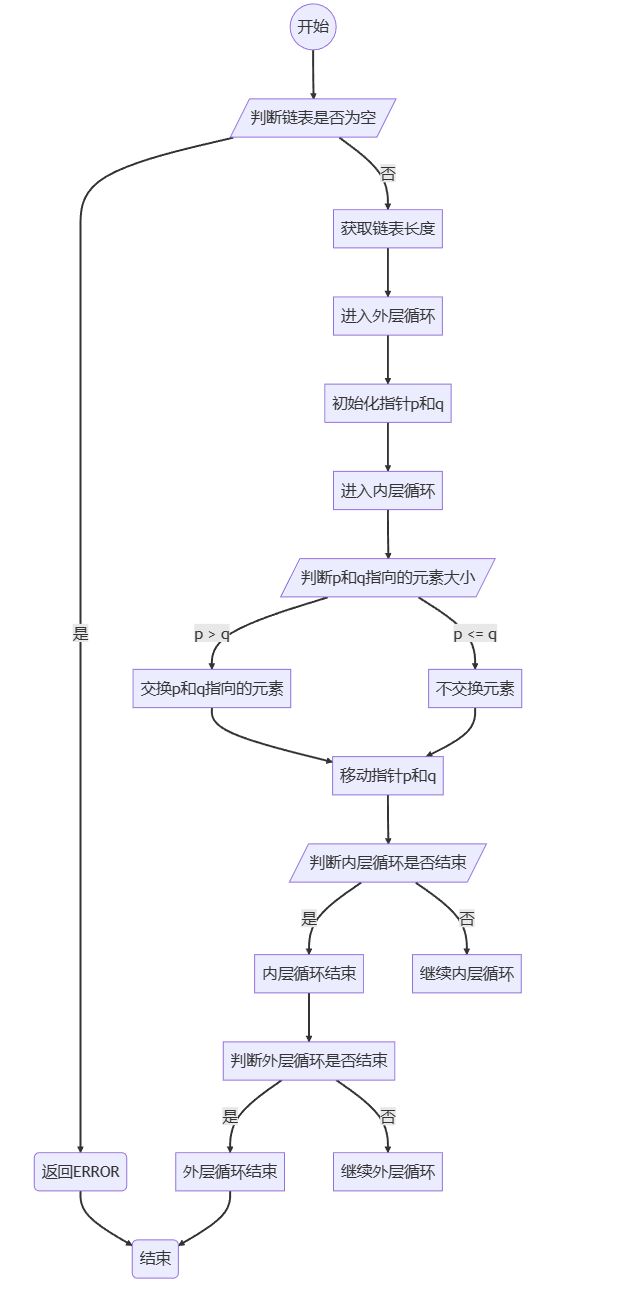
\includegraphics[width=\textwidth]{images/排序表.png}
%	\caption{排序线性表}
%	\label{fig1-2}
%\end{figure}
\begin{figure}[H]
	\centering
	\begin{minipage}{0.7\linewidth}
		\centering
		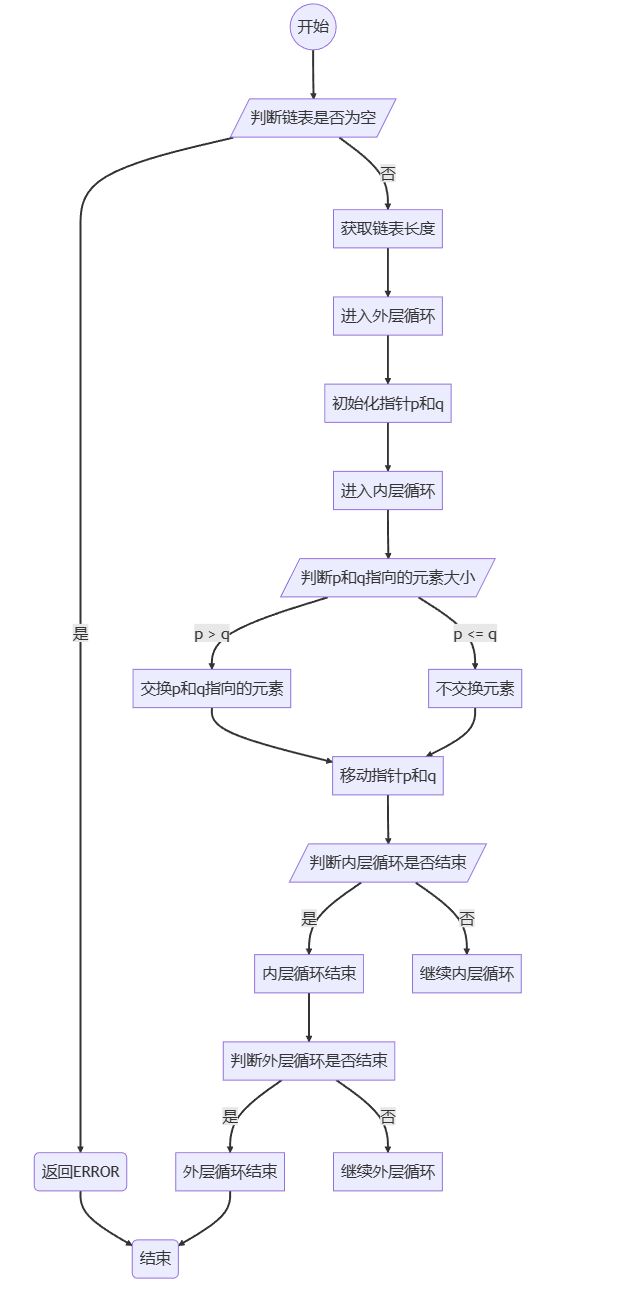
\includegraphics[width=0.9\linewidth]{images/排序表.png}
	\end{minipage}
	\caption{排序线性表}
	\label{fig1-3}
\end{figure}


	\item 删除倒数第n个元素\\
	函数名称是RemoveNthFromEnd(L,n); 初始条件是线性表L已存在且非空, 操作结果是该链表中倒数第n个节点;
	如果线性表不存在,返回不可行。否则遍历链表求出表长,根据表长获得倒数第n个元素的索引,
	根据这个索引遍历链表寻找删除位置,如果索引不大于0,返回索引错误,如果遍历完成后依然未找到,返回索引错误。
	否则删除节点。
	
	复杂度:时间复杂度 T(n) = O(n)
		%\begin{figure}[h]
		%\begin{center}
		%	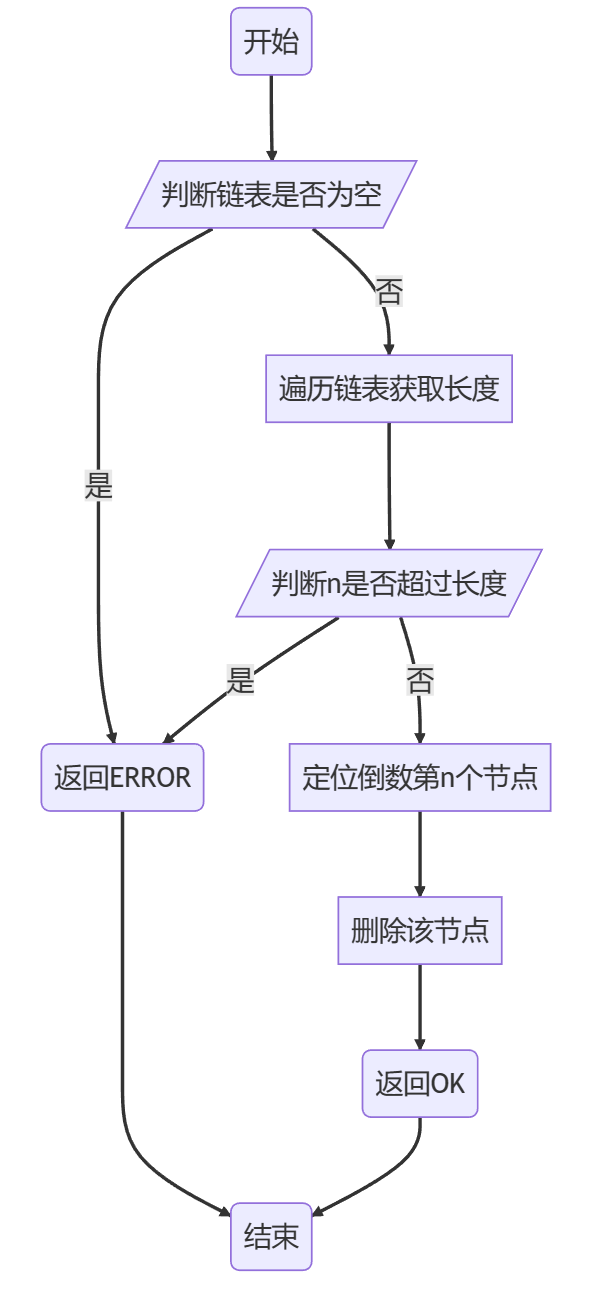
\includegraphics[width=\textwidth]{images/删除倒数节点.png}
		%	\caption{删除倒数第n个元素}
		%	\label{fig1-3}
	%	\end{center}
%	\end{figure}
	\begin{figure}[H]
		\centering
		\begin{minipage}{0.7\linewidth}
			\centering
			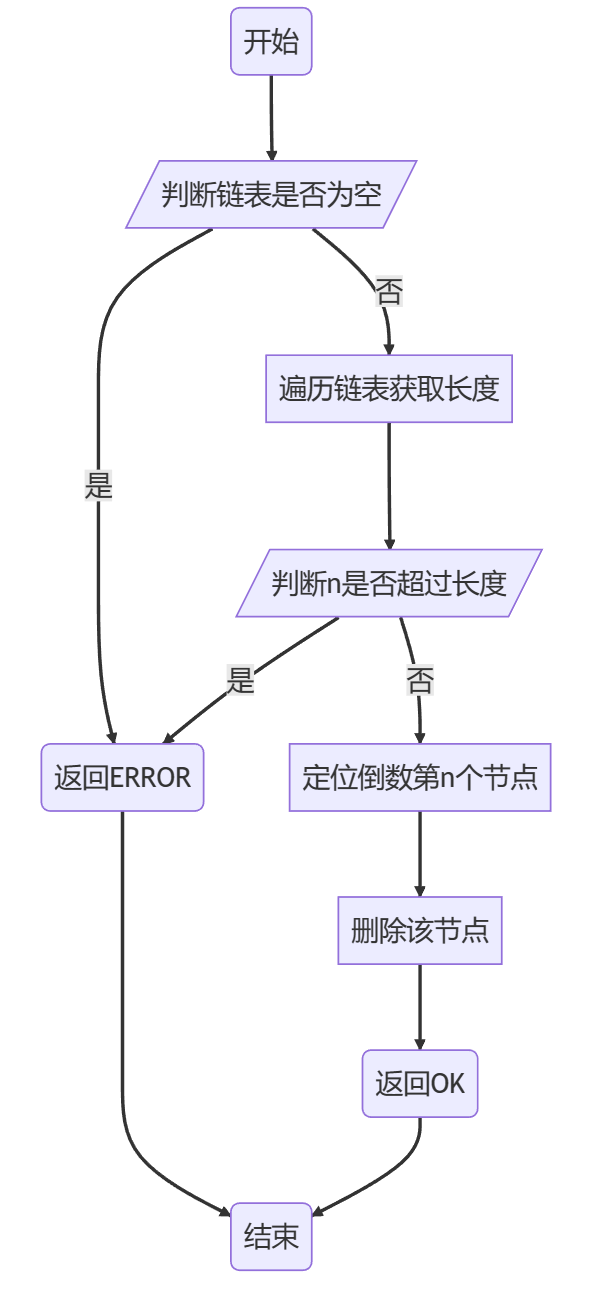
\includegraphics[width=0.9\linewidth]{images/删除倒数节点.png}
		\end{minipage}
		\caption{删除倒数第n个元素}
		\label{fig1-4}
	\end{figure}
	%\newpage
	\item 线性表的文件操作\\
	如果线性表不存在,返回不可行。打开只写文件,遍历线性表并依次写入元素。销毁线性表。接着初始化线性表,
	以只读模式打开刚才保存的文件,依次读入各元素,新建节点并插入线性表,直到读取到EOF。
	
	\emph{复杂度:时间复杂度 T(n) = O(1)}
%	\begin{figure}[h]
%		\begin{center}
%			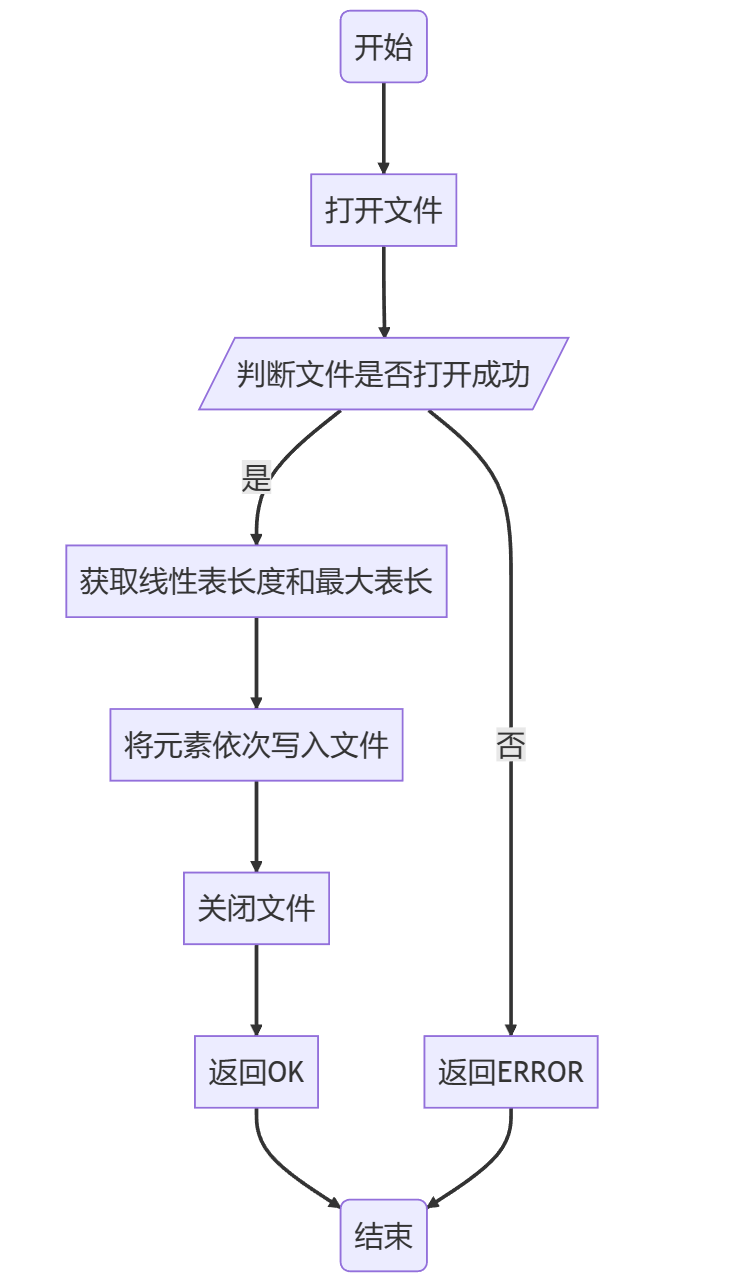
\includegraphics[width=\textwidth]{images/文件保存.png}
%			\caption{文件保存}
%			\label{fig1-4}
%		\end{center}
%	\end{figure}
%\begin{figure}[h]
%	\begin{center}
%		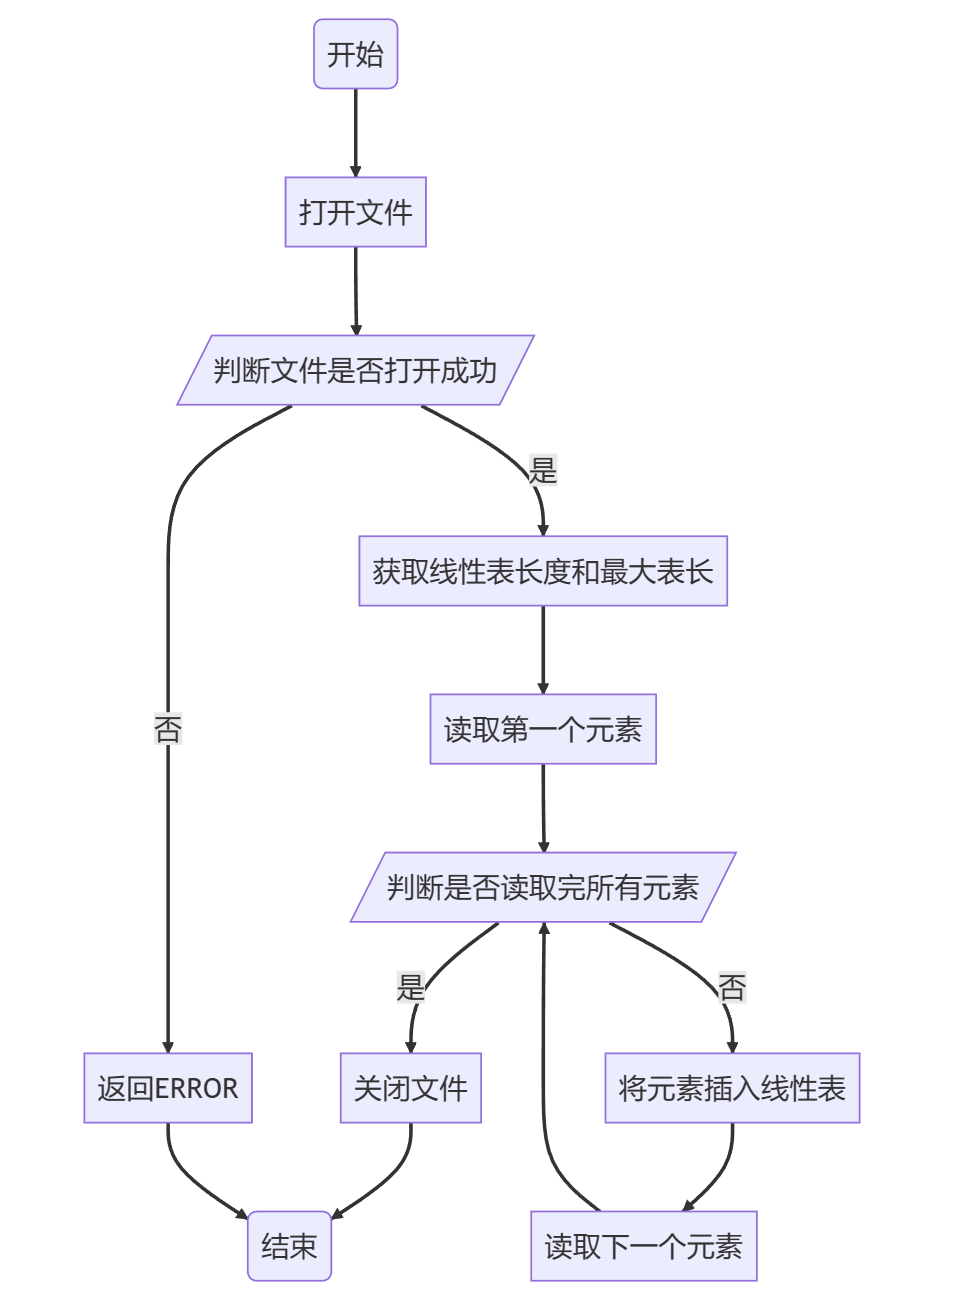
\includegraphics[width=\textwidth]{images/文件读取.png}
%		\caption{文件读取}
%		\label{fig1-5}
%	\end{center}
%\end{figure}
	\begin{figure}[H]
	\centering
	\begin{minipage}{0.7\linewidth}
		\centering
		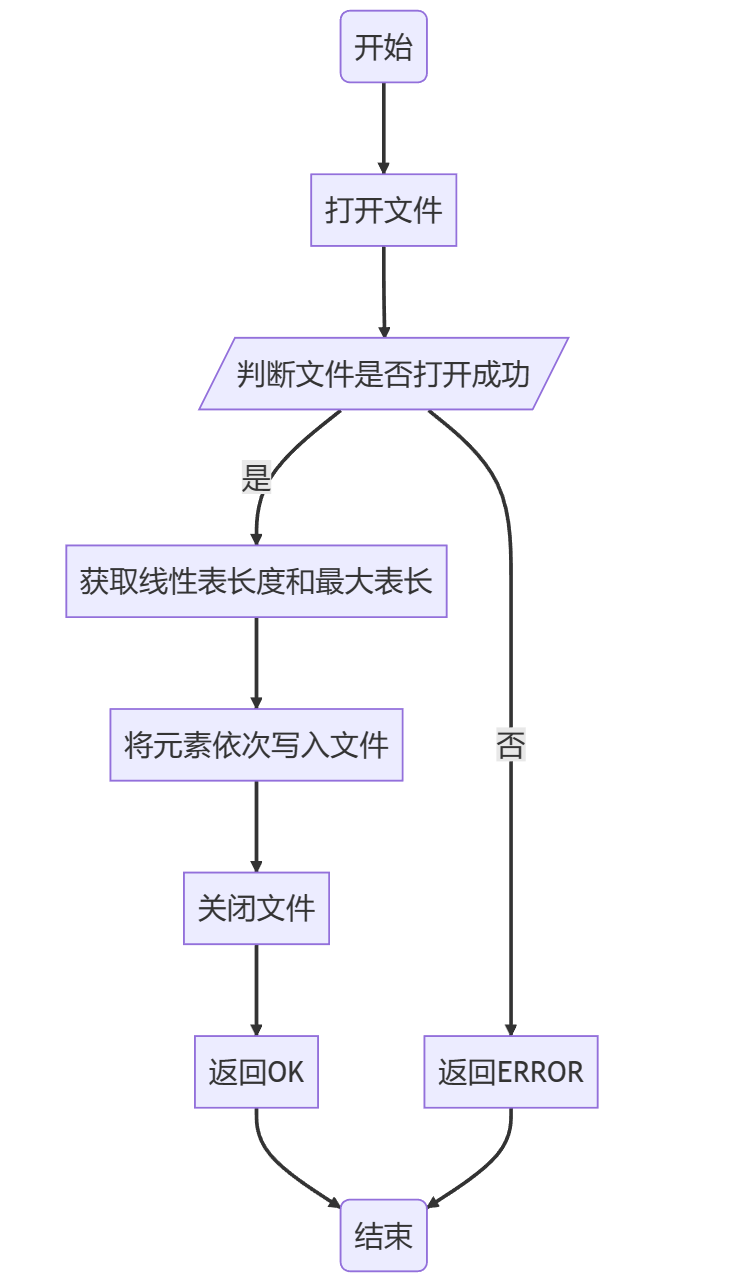
\includegraphics[width=0.9\linewidth]{images/文件保存.png}
	\end{minipage}
	\caption{文件保存}
	\label{fig1-5}
\end{figure}

\begin{figure}[H]
	\centering
	\begin{minipage}{0.7\linewidth}
		\centering
		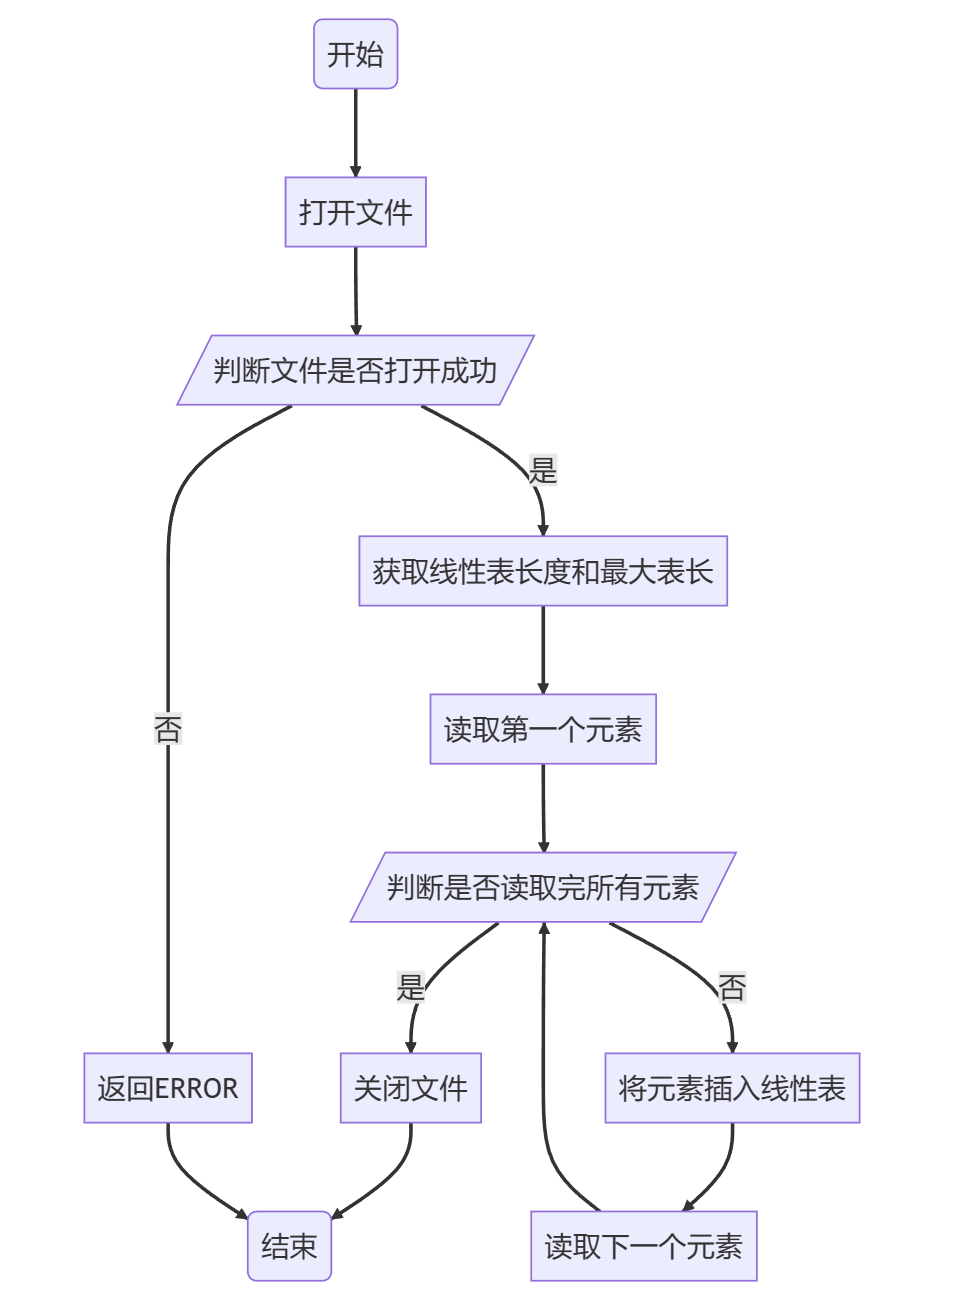
\includegraphics[width=0.9\linewidth]{images/文件读取.png}
	\end{minipage}
	\caption{文件读取}
	\label{fig1-6}
\end{figure}
%\newpage
	\item 实现多个线性表管理:设计相应的数据结构管理多个线性表的查找、添加、移除等功能。
	
	针对多线性表的管理,实验设计一个新的结构体,其中定义了本实验链表的一个结构体数组,本质上是通过数组存储多个链表以此实现多线性表的管理,针对数组中每个线性表的管理
	和上述基础功能对单个链表的操作基本一致,不同在于,我们需要实现不同链表的切换,即找寻并切换至目标链表进行管理。
	
	在设计过程中每一个链表都有一个name数组对链表以及对应的位序,因此,我们可以更改序号来切换不同链表,若没有找到目标或者查找的序号超过链表数组的最大数量,则返返回ERROR。
	
	复杂度:时间复杂度 T(n) = O(1)
%	\begin{figure}[h]
%		\begin{center}
%			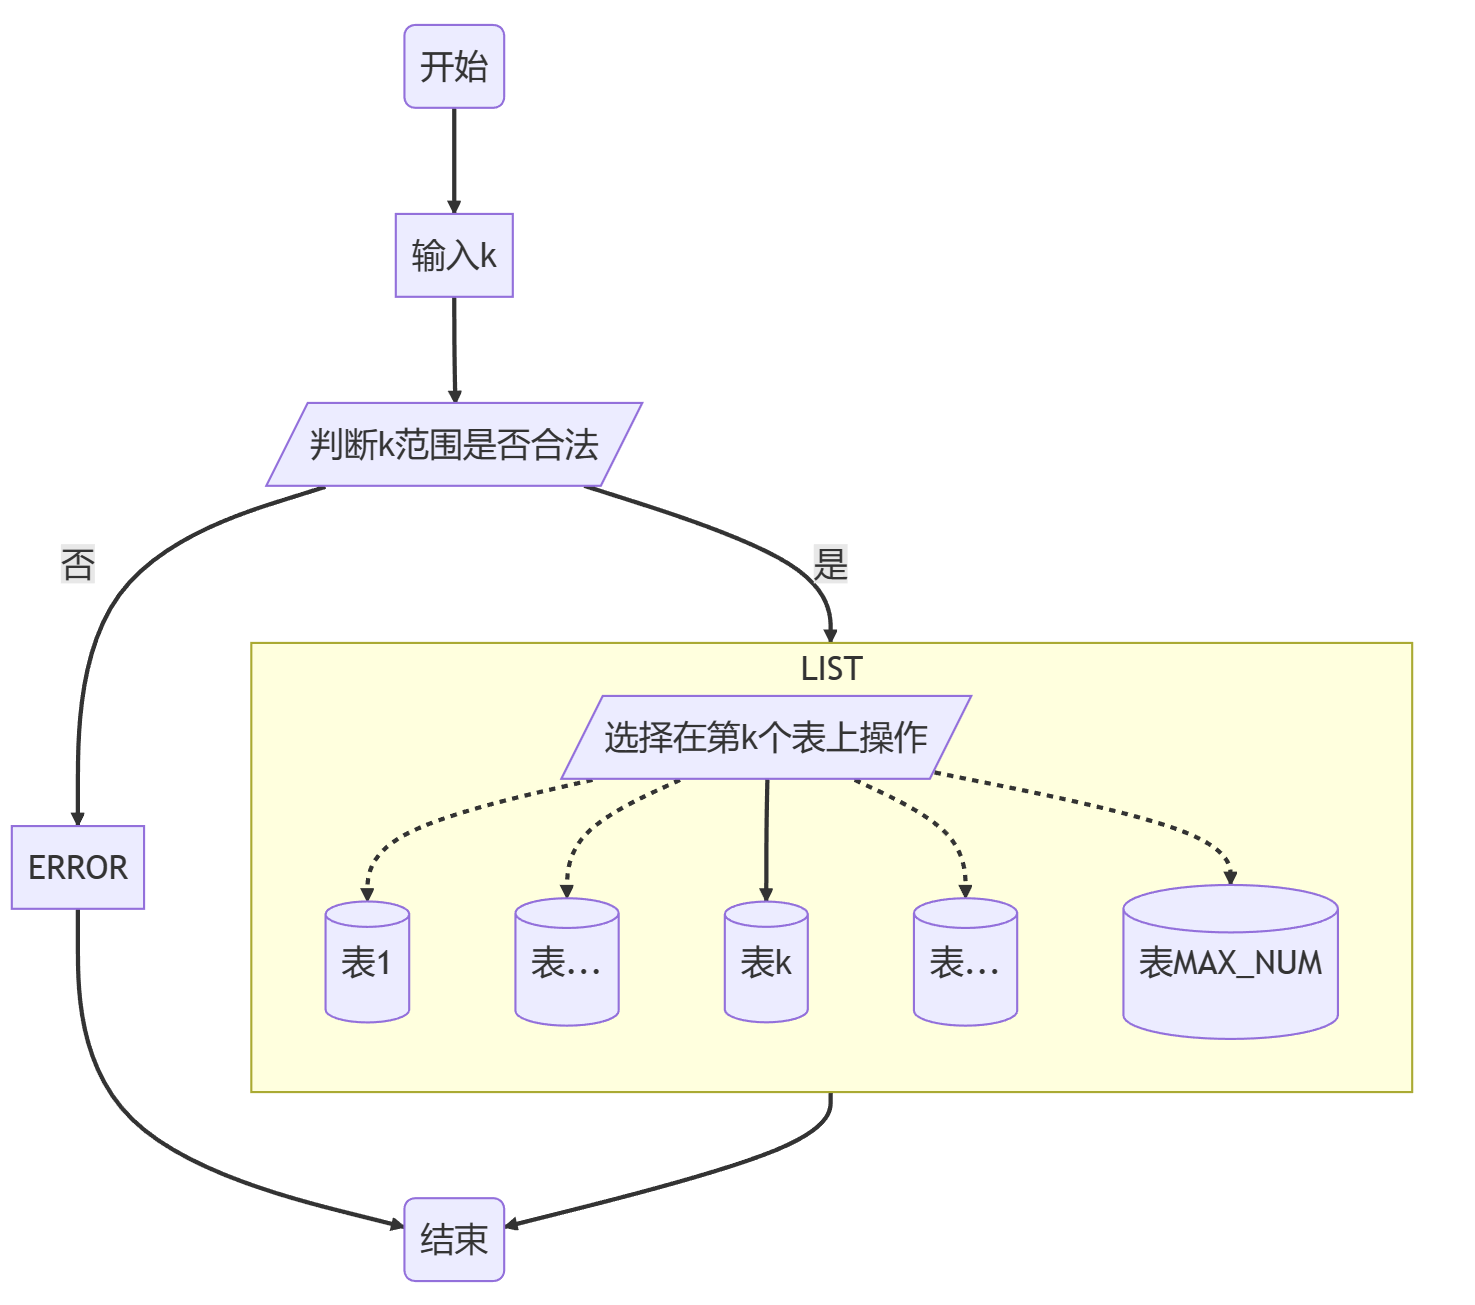
\includegraphics[width=\textwidth]{images/多表管理.png}
%			\caption{多表线性表管理的实现}
%			\label{fig1-6}
%		\end{center}
%	\end{figure}
	\begin{figure}[H]
	\centering
	\begin{minipage}{0.8\linewidth}
		\centering
		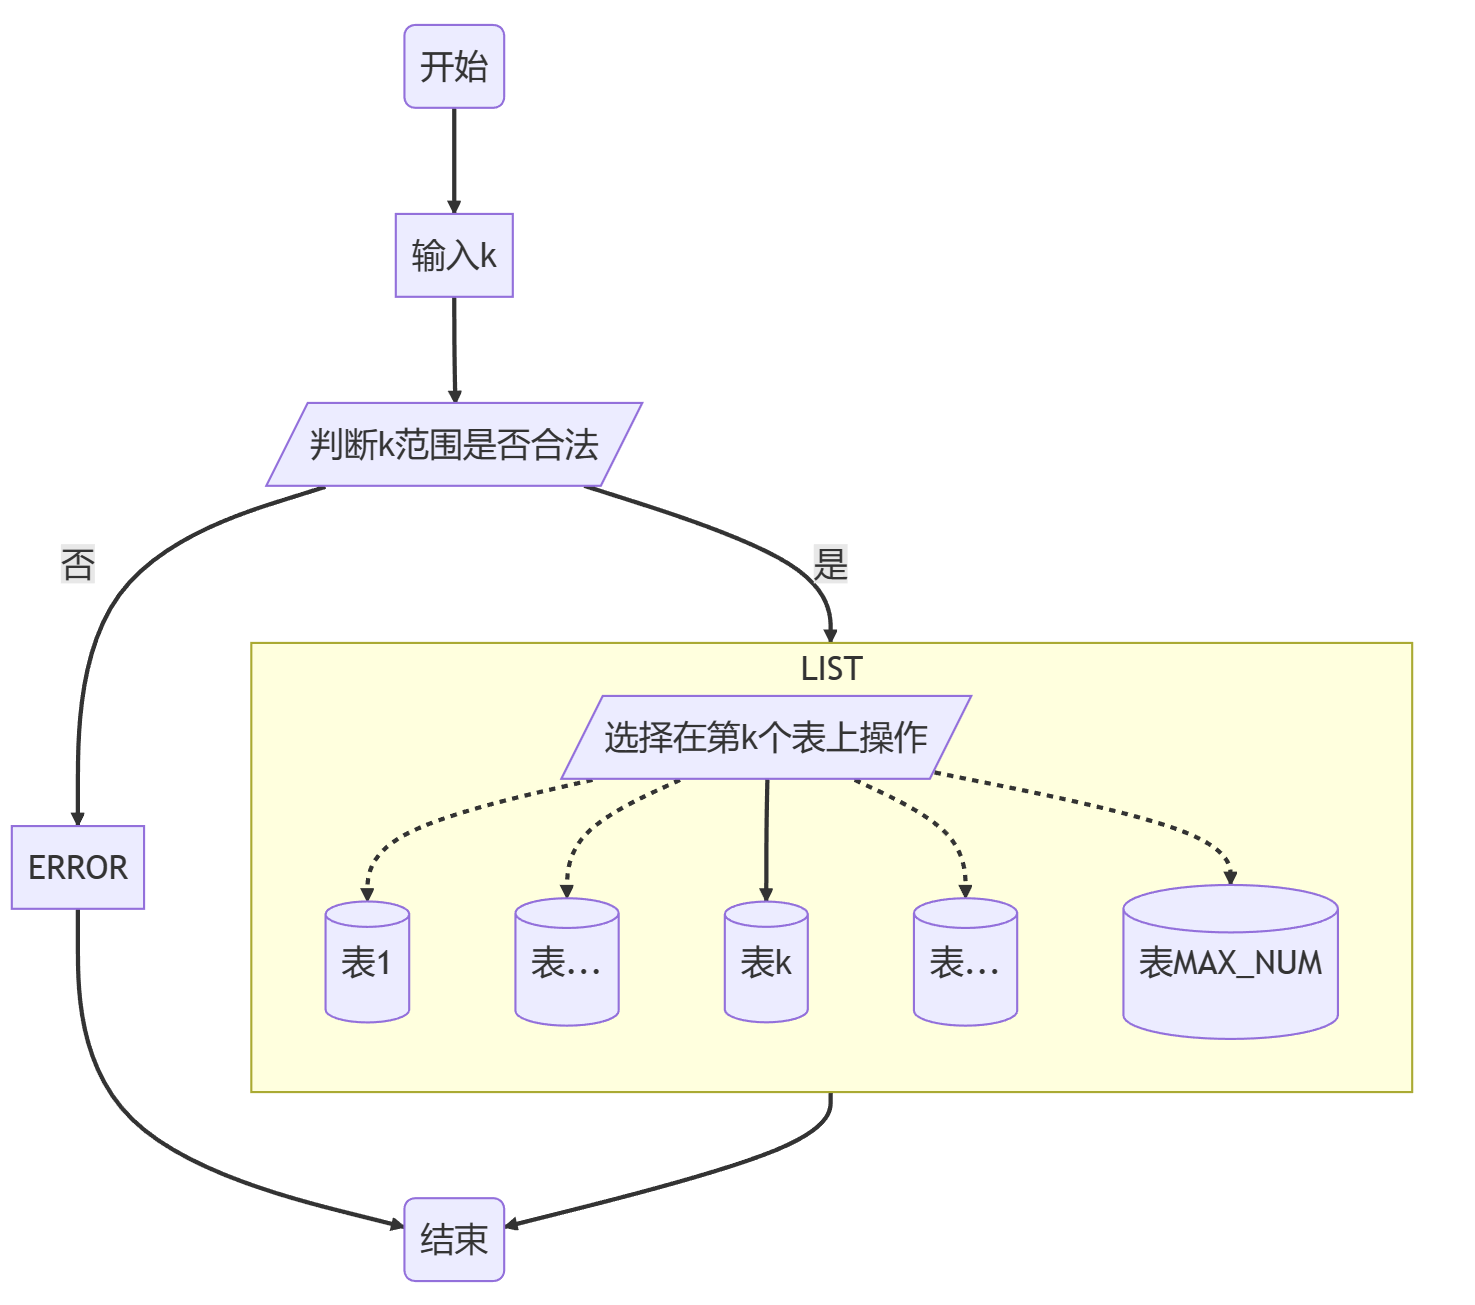
\includegraphics[width=0.9\linewidth]{images/多表管理.png}
	\end{minipage}
	\caption{多表线性表管理的实现}
	\label{fig1-7}
	\end{figure}
	\newpage
	
\end{enumerate}
\subsection{系统测试}
以下主要说明针对各个函数正常和异常的测试用例及测试结果。
	\begin{enumerate}
		\item 初始化线性表\\
		若线性表未初始化,输出结果如下图:
			\begin{figure}[H]
			\centering
			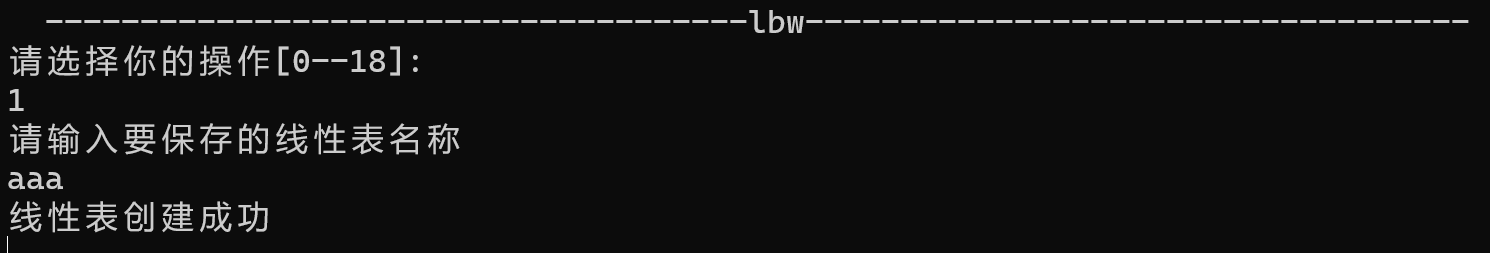
\includegraphics[width=1\linewidth]{images/初始化成功.png}
			\caption{初始化成功}
			\label{fig1-8}
		\end{figure}
	若线性表已初始化,输出结果如下图:
	\begin{figure}[H]
		\centering
		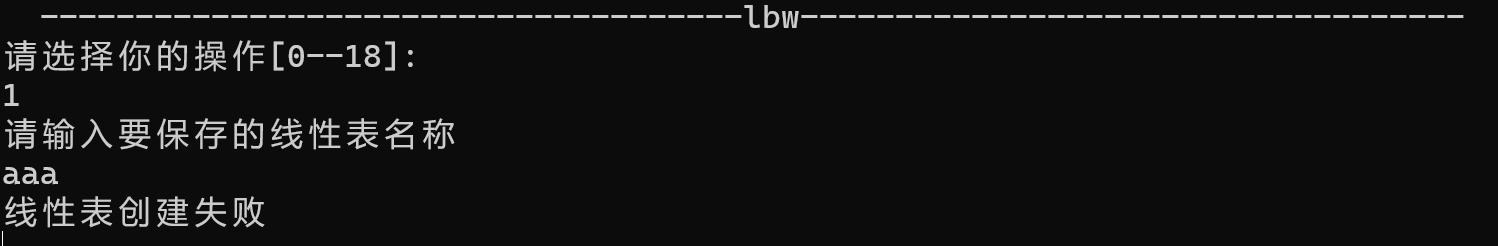
\includegraphics[width=1\linewidth]{images/初始化失败.png}
		\caption{初始化失败}
		\label{fig1-9}
	\end{figure}

		\item 销毁线性表\\
		若线性表未销毁,输出结果如下图:
		\begin{figure}[H]
			\centering
			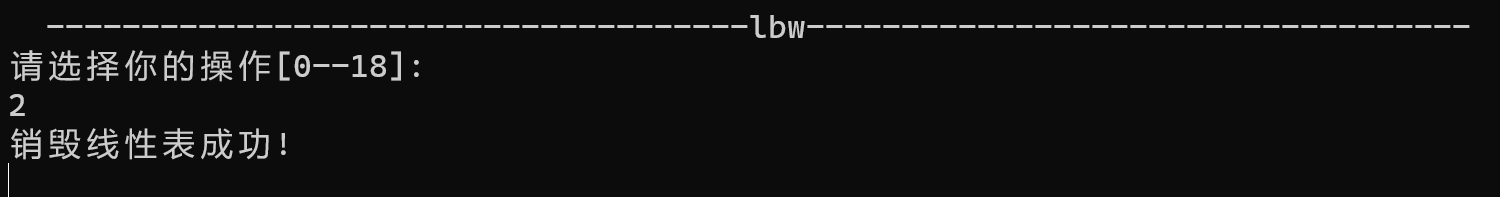
\includegraphics[width=1\linewidth]{images/销毁成功.png}
			\caption{销毁成功}
			\label{fig1-10}
		\end{figure}
		若线性表已销毁,输出结果如下图:
		\begin{figure}[H]
			\centering
			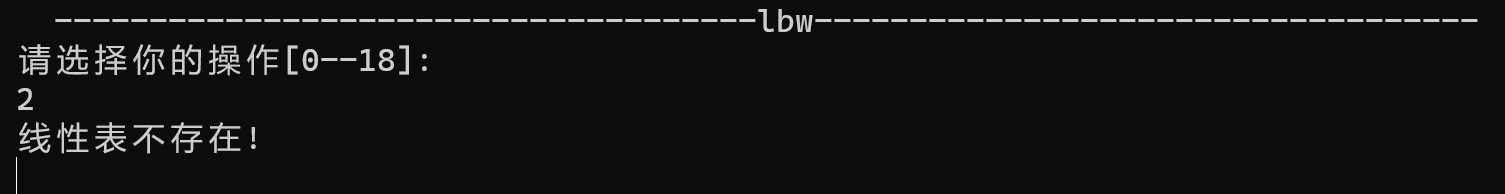
\includegraphics[width=1\linewidth]{images/销毁失败.png}
			\caption{销毁失败}
			\label{fig1-11}
		\end{figure}
		\item 清空线性表\\
		若线性表未清空,输出结果如下图:
		\begin{figure}[H]
			\centering
			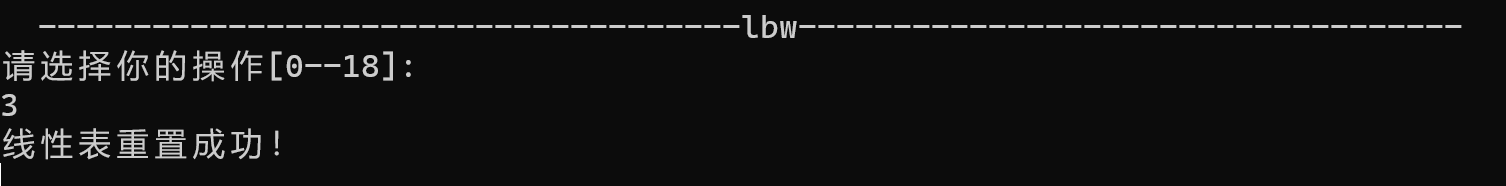
\includegraphics[width=1\linewidth]{images/清空成功.png}
			\caption{清空成功}
			\label{fig1-12}
		\end{figure}
			若线性表已清空,输出结果如下图:
			\begin{figure}[H]
				\centering
				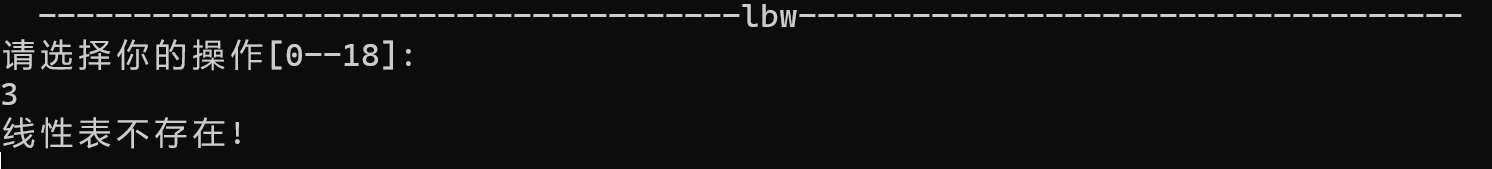
\includegraphics[width=1\linewidth]{images/清空失败.png}
				\caption{清空失败}
				\label{fig1-13}
			\end{figure}
		\item 判定线性表是否为空\\
		若线性表为空表,输出结果如下图:
		\begin{figure}[H]
			\centering
			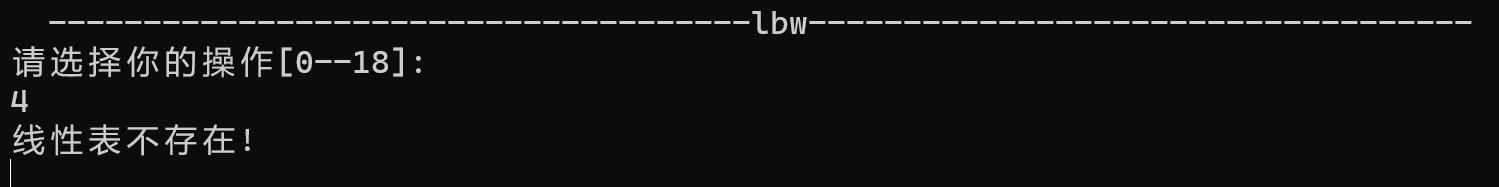
\includegraphics[width=1\linewidth]{images/判空失败.png}
			\caption{判空失败}
			\label{fig1-14}
		\end{figure}
		若线性表不为空表,输出结果如下图:
	\begin{figure}[H]
		\centering
		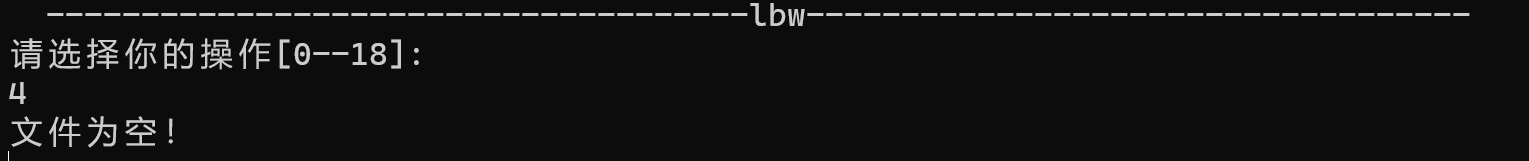
\includegraphics[width=1\linewidth]{images/判空成功.png}
		\caption{判空成功}
		\label{fig1-15}
	\end{figure}
		\item 求线性表的长度\\
		输入[1],输出结果如下图:
		\begin{figure}[H]
			\centering
			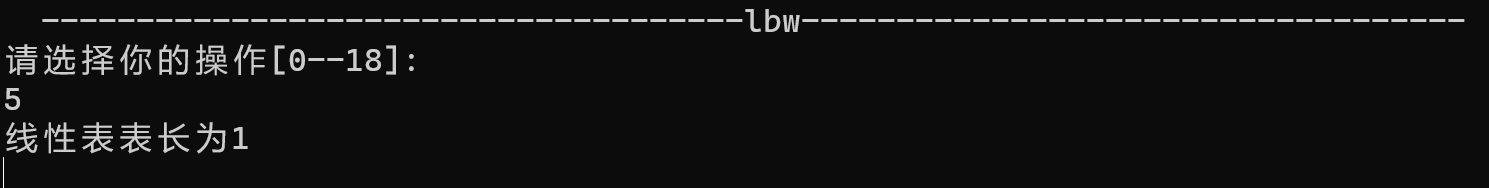
\includegraphics[width=1\linewidth]{images/求长度1.png}
			\caption{求非空表的表长}
			\label{fig1-16}
		\end{figure}
	若线性表为空表,输出结果如下图:
	\begin{figure}[H]
		\centering
		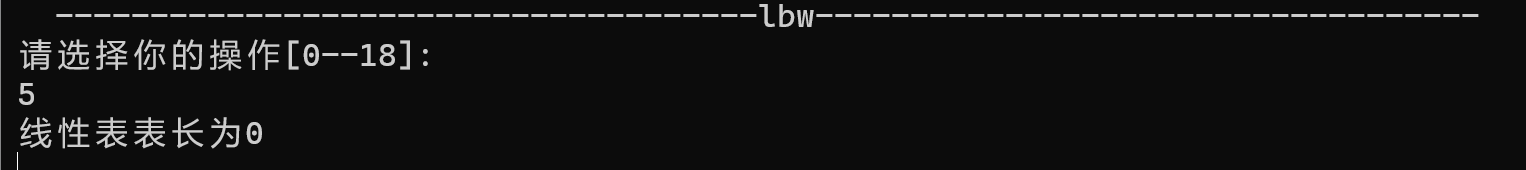
\includegraphics[width=1\linewidth]{images/求长度0.png}
		\caption{求空表的表长}
		\label{fig1-17}
	\end{figure}
		\item 获取元素\\
		输入[1],索引1,输出结果如下图:
		\begin{figure}[H]
			\centering
			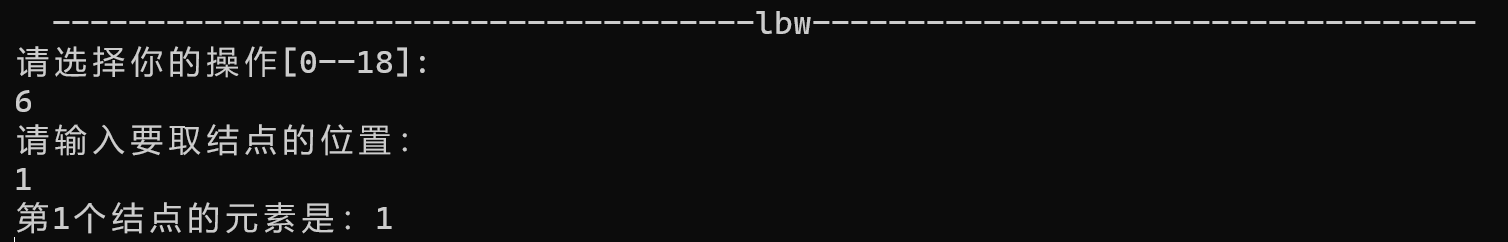
\includegraphics[width=1\linewidth]{images/取元素成功.png}
			\caption{获取元素成功}
			\label{fig1-18}
		\end{figure}
			输入[1],索引0,输出结果如下图:
	\begin{figure}[H]
		\centering
		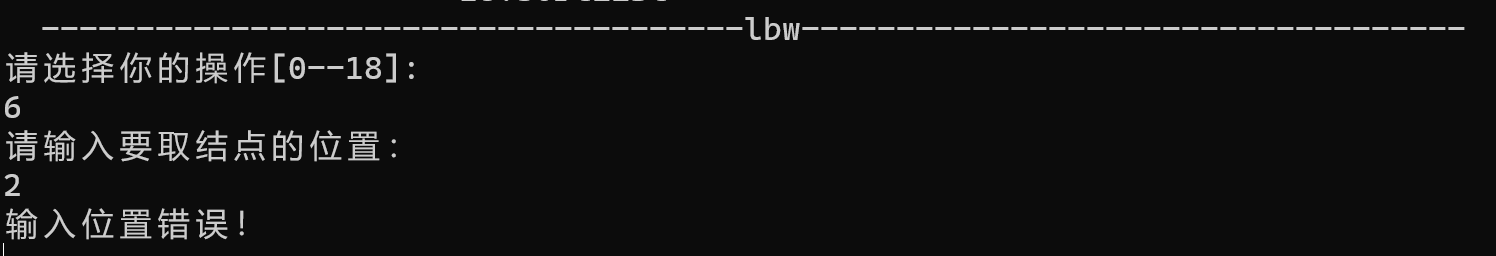
\includegraphics[width=1\linewidth]{images/取元素不合法.png}
		\caption{获取元素失败}
		\label{fig1-18}
	\end{figure}

		\item 查找元素\\
		输入[1,-2,3,4],查找1,输出结果如下图:
		\begin{figure}[H]
			\centering
			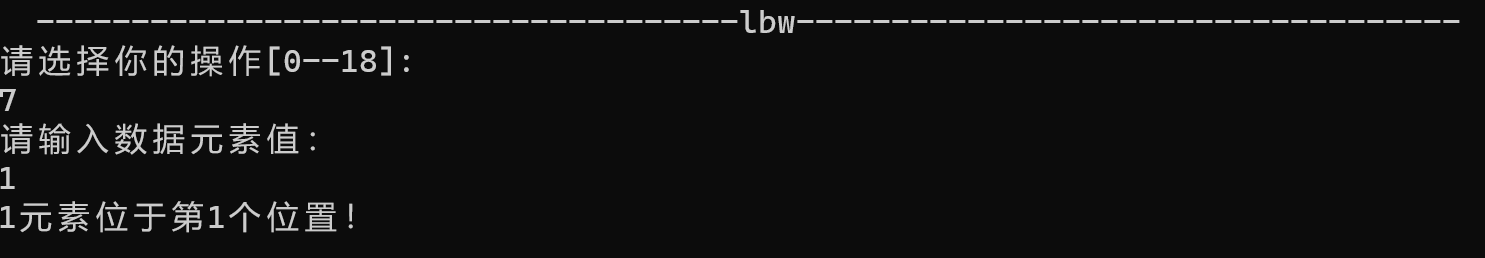
\includegraphics[width=1\linewidth]{images/定位元素成功.png}
			\caption{查找元素成功}
			\label{fig1-19}
		\end{figure}
		输入[1,-2,3,4],查找2,输出结果如下图:
		
		\begin{figure}[H]
			\centering
			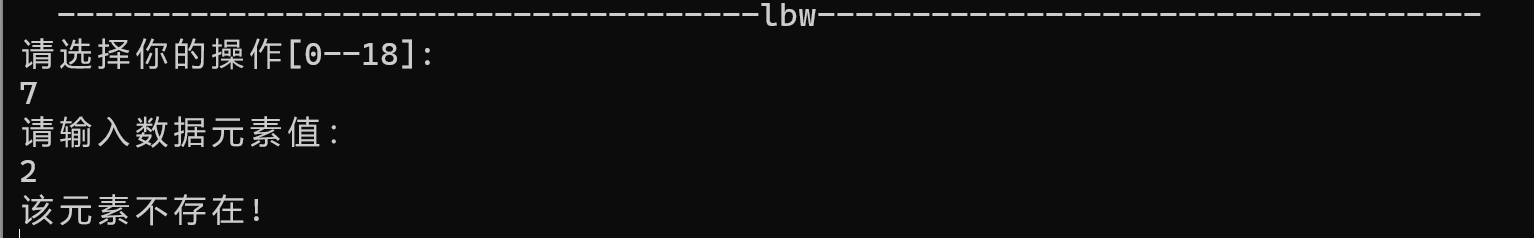
\includegraphics[width=1\linewidth]{images/定位元素失败.png}
			\caption{查找元素失败}
			\label{fig1-20}
		\end{figure}
		\item 获取前驱元素\\
		输入[1,2,3,4],查找2的前驱元素,输出结果如下图:
		\begin{figure}[H]
			\centering
			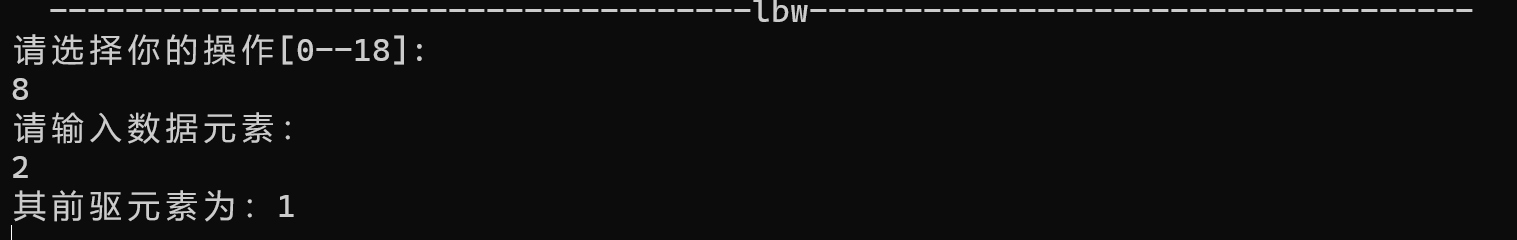
\includegraphics[width=1\linewidth]{images/前驱元素存在.png}
			\caption{查找前驱元素成功}
			\label{fig1-21}
		\end{figure}
		输入[1,2,3,4],查找1前驱元素,输出结果如下图:
		\begin{figure}[H]
			\centering
			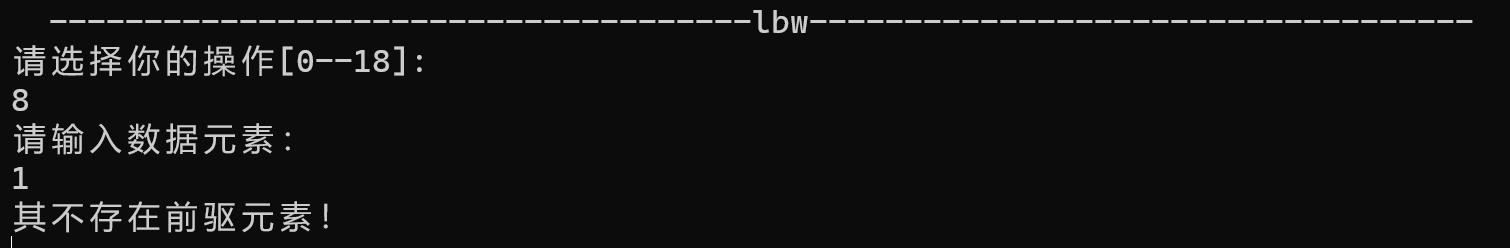
\includegraphics[width=1\linewidth]{images/前驱元素不存在.png}
			\caption{查找前驱元素失败}
			\label{fig1-22}
		\end{figure}
		\item 获取后继元素\\
		输入[1,2],查找1的后继元素,输出结果如下图:
		\begin{figure}[htbp]
			\centering
			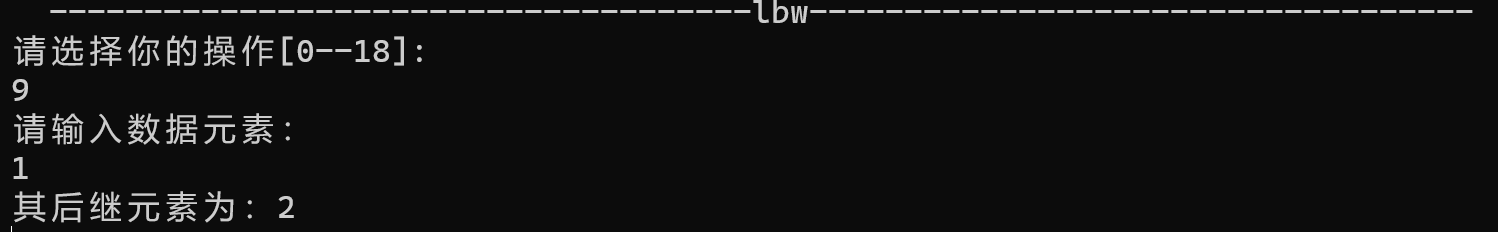
\includegraphics[width=1\linewidth]{images/后继元素存在.png}
			\caption{查找后继元素成功}
			\label{fig1-23}
		\end{figure}
	
		输入[1,2],查找2的后继元素,输出结果如下图:
		\begin{figure}[htbp]
			\centering
			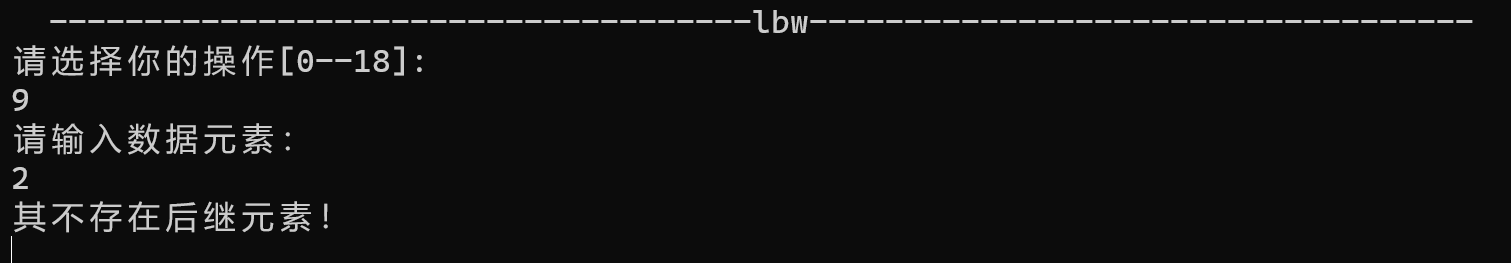
\includegraphics[width=1\linewidth]{images/后继元素不存在.png}
			\caption{查找后继元素失败}
			\label{fig1-24}
		\end{figure}
		\item 插入元素\\
		输入[1,2],插入元素3到位置3,输出结果如下图:
		\begin{figure}[htbp]
			\centering
			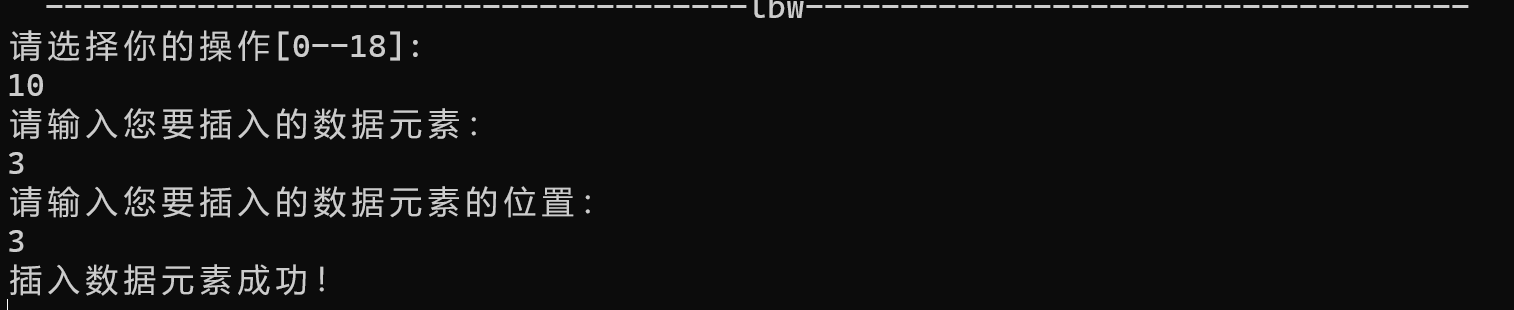
\includegraphics[width=1\linewidth]{images/插入成功.png}
			\caption{插入元素成功}
			\label{fig1-25}
		\end{figure}
		
		输入[1,2],插入元素3到位置4,输出结果如下图:
		\begin{figure}[H]
			\centering
			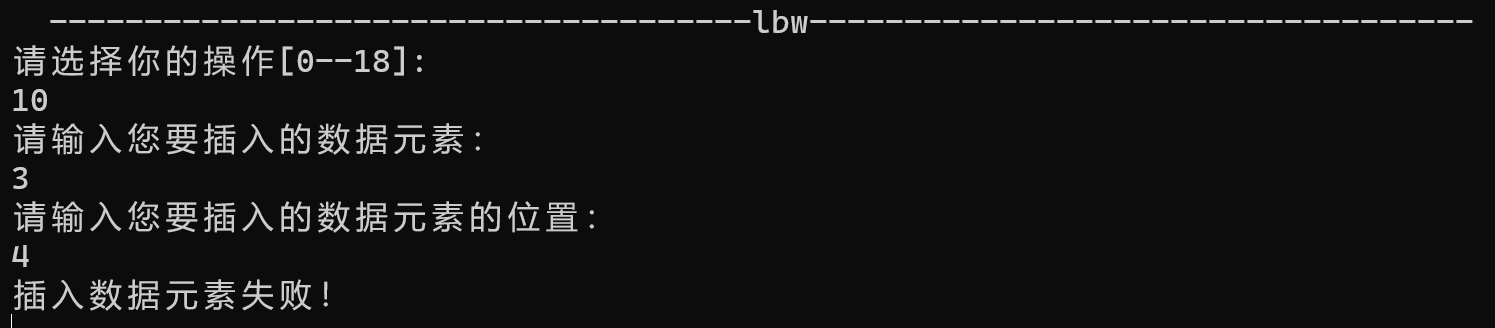
\includegraphics[width=1\linewidth]{images/插入失败.png}
			\caption{插入元素失败}
			\label{fig1-26}
		\end{figure}
	
		\item 删除元素\\
		输入[1,2,3],删除位置3上的元素,输出结果如下图:
		\begin{figure}[H]
			\centering
			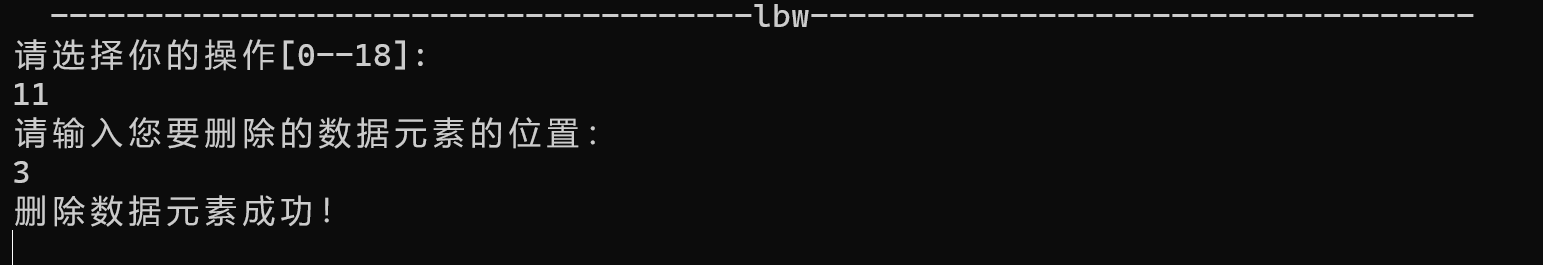
\includegraphics[width=1\linewidth]{images/删除成功.png}
			\caption{删除元素成功}
			\label{fig1-27}
		\end{figure}
	
	输入[1,2,3],删除位置0上的元素,输出结果如下图:
	\begin{figure}[H]
		\centering
		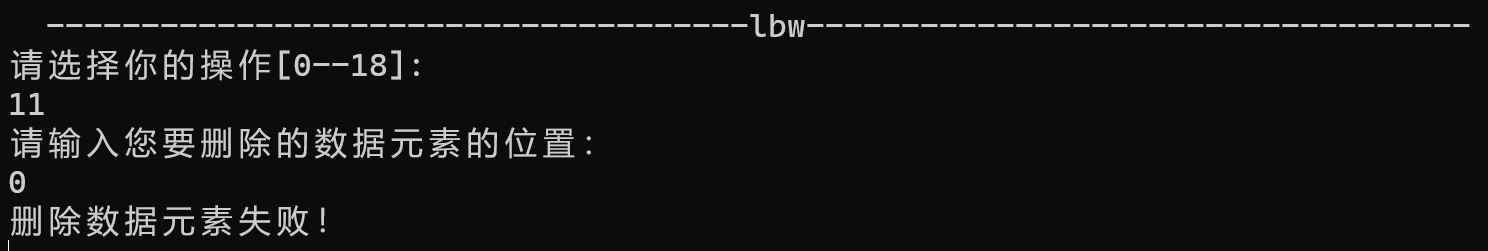
\includegraphics[width=1\linewidth]{images/删除失败.png}
		\caption{删除元素失败}
		\label{fig1-28}
	\end{figure}

		\item 遍历线性表\\
		输入[1,2],遍历结果如下图:
			\begin{figure}[H]
			\centering
			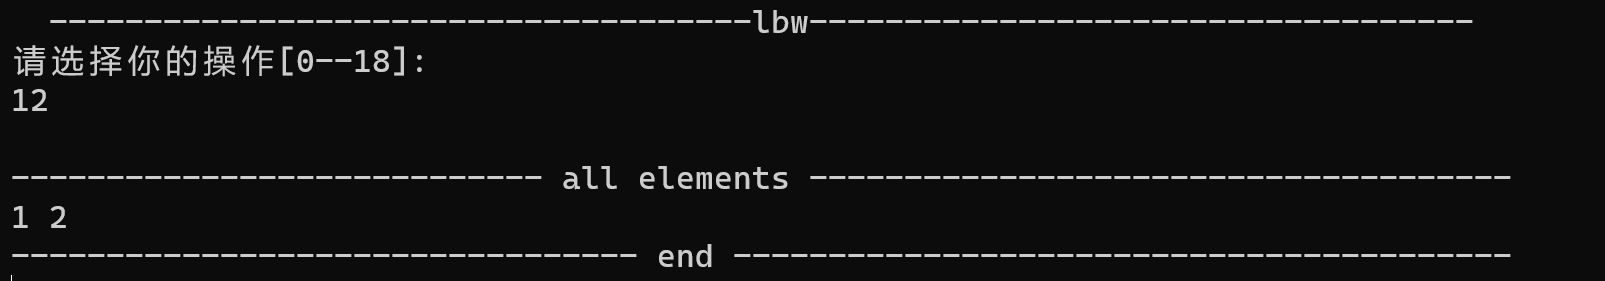
\includegraphics[width=1\linewidth]{images/遍历成功.png}
			\caption{遍历线性表成功}
			\label{fig1-29}
		\end{figure}
		\item 翻转线性表\\
		输入[1,2,3,4,-5,-4],输出结果如下图:
		\begin{figure}[H]
			\centering
			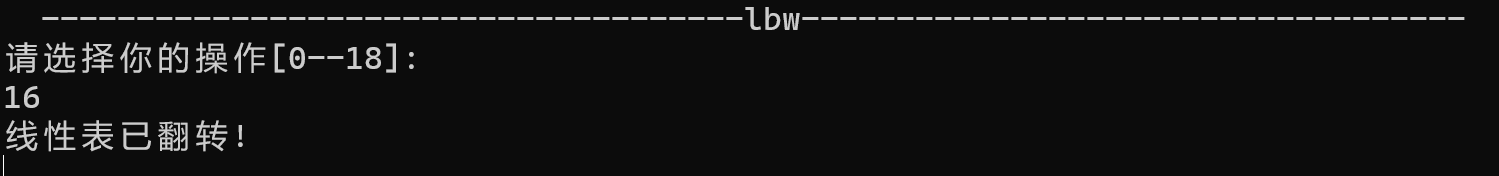
\includegraphics[width=1\linewidth]{images/翻转成功.png}
			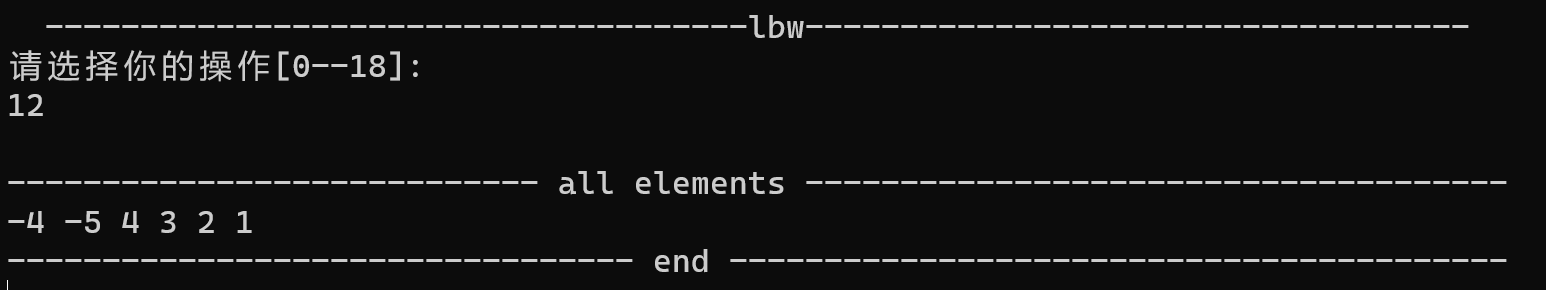
\includegraphics[width=1\linewidth]{images/翻转结果.png}
			\caption{翻转线性表成功}
			\label{fig1-30}
		\end{figure}
	
		\item 排序线性表\\
		输入[1,3,4,-5,-4],输出结果如下图:
		\begin{figure}[H]
			\centering
			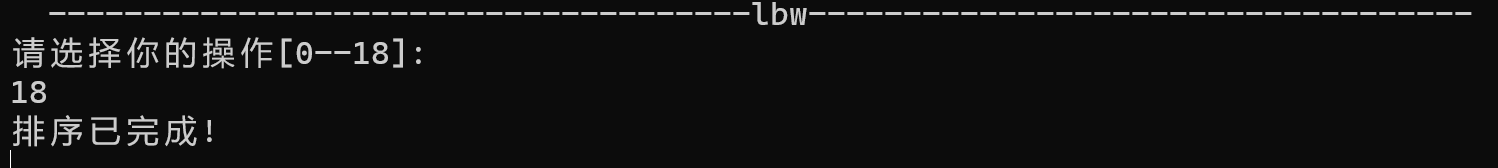
\includegraphics[width=1\linewidth]{images/排序成功.png}
			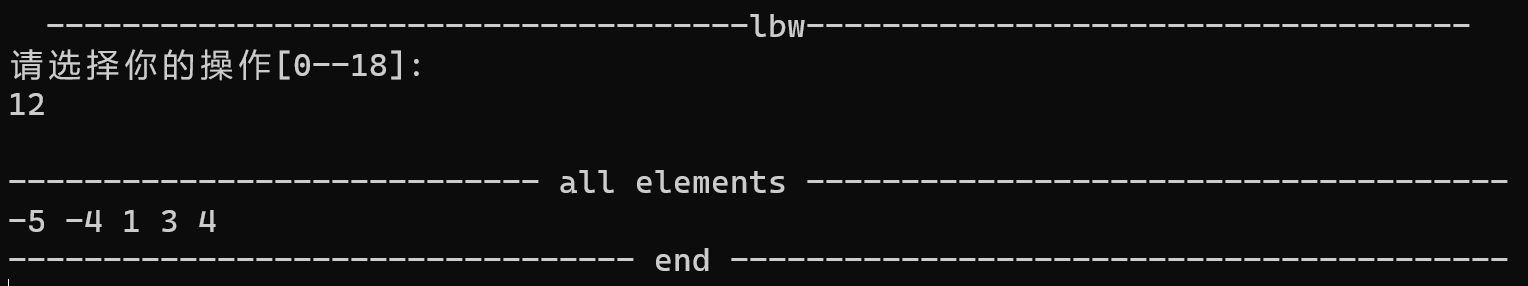
\includegraphics[width=1\linewidth]{images/排序结果.png}
			\caption{排序线性表成功}
			\label{fig1-31}
		\end{figure}
		\item 删除倒数第n个元素\\
		输入[-4,-5,4,3,2,1],删除倒数第2个元素,输出结果如下图:
		\begin{figure}[H]
			\centering
			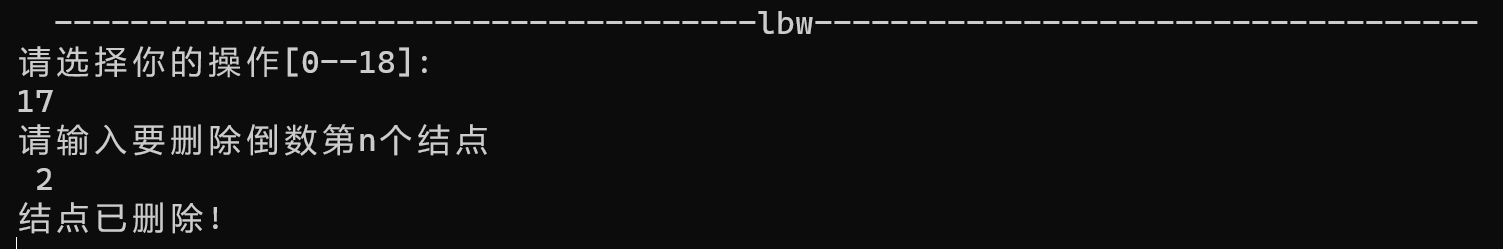
\includegraphics[width=1\linewidth]{images/从后删除成功.png}
			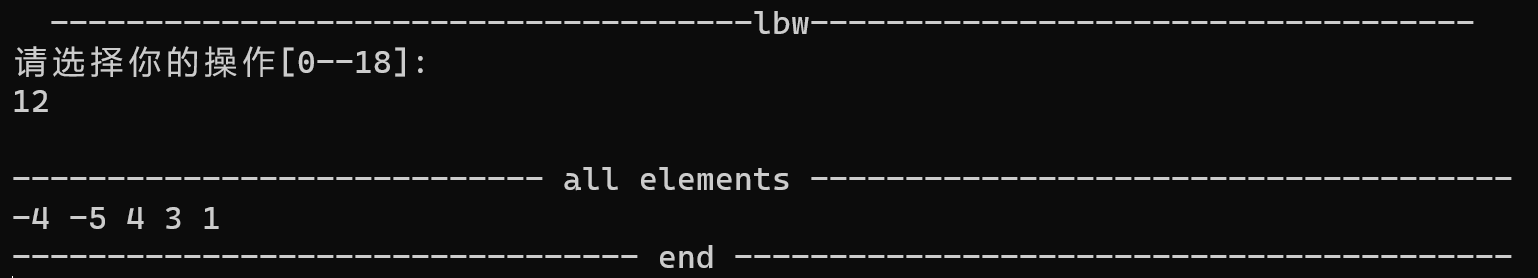
\includegraphics[width=1\linewidth]{images/从后删除结果.png}
			\caption{删除倒数第n个元素成功}
			\label{fig1-32}
		\end{figure}
	
		输入[-4,-5,4,3,2,1],删除倒数第7个元素,输出结果如下图:
		\begin{figure}[H]
			\centering
			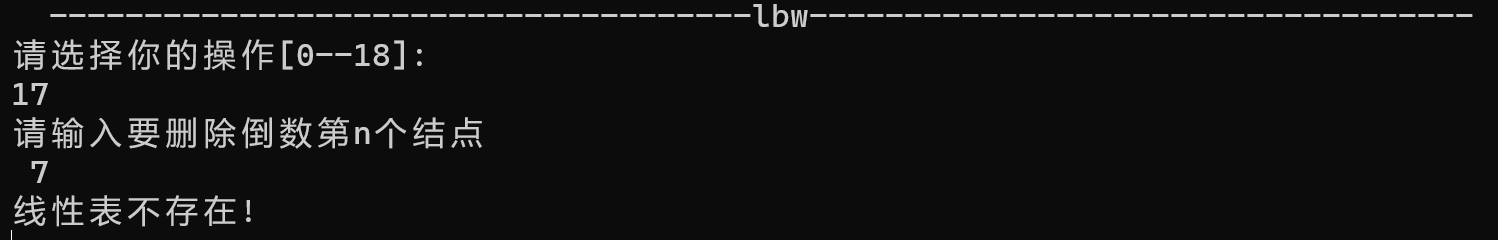
\includegraphics[width=1\linewidth]{images/从后删除失败.png}
			\caption{删除倒数第n个元素失败}
			\label{fig1-33}
		\end{figure}
		
		\item 线性表的文件操作\\
		文件保存:输入[1,2,3,4],保存为test.txt文件,文件内容如下:
		\begin{figure}[H]
			\centering
			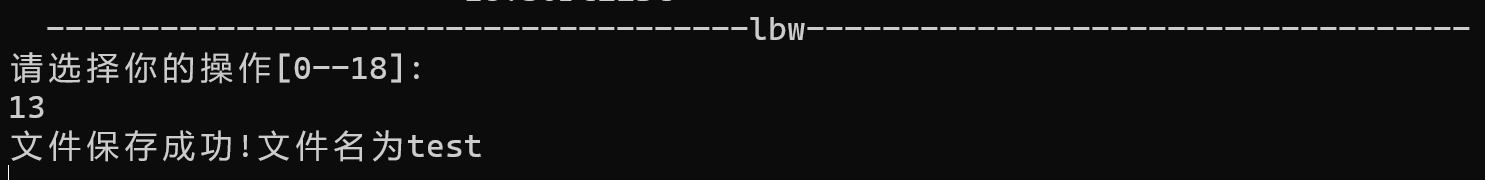
\includegraphics[width=1\linewidth]{images/文件操作成功.png}
			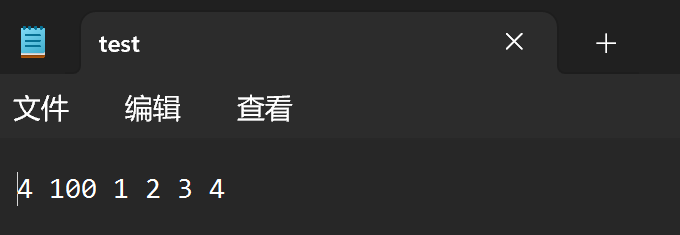
\includegraphics[width=1\linewidth]{images/文件操作结果.png}
			\caption{文件保存}
			\label{fig1-34}
		\end{figure}
	
		文件读取:初始化表后,我们读入test.txt文件,输出结果如下图:
		\begin{figure}[H]
			\centering
			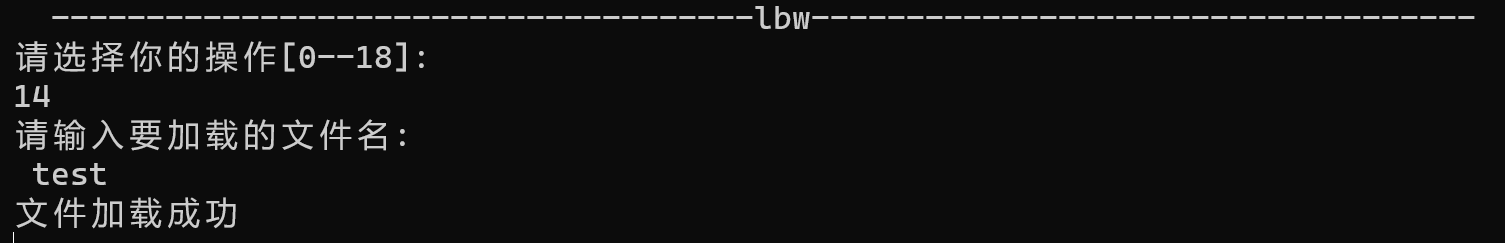
\includegraphics[width=1\linewidth]{images/文件加载成功.png}
			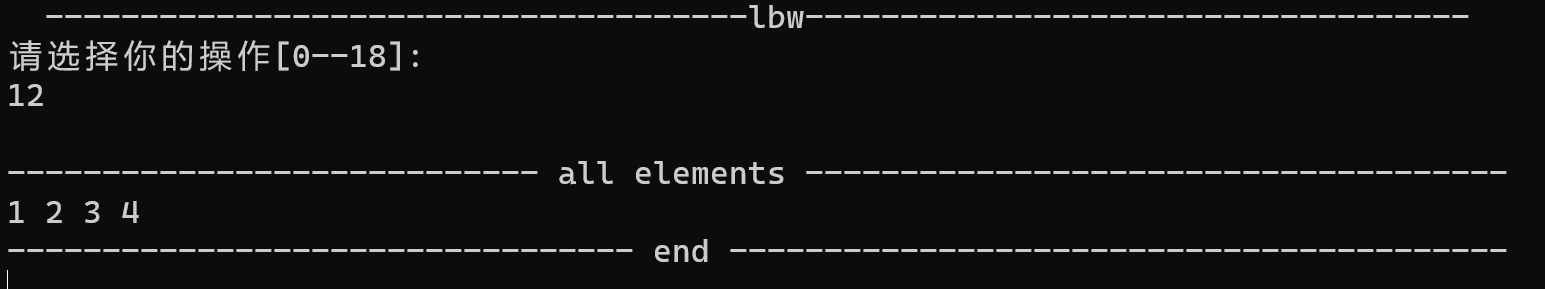
\includegraphics[width=1\linewidth]{images/文件加载结果.png}
			\caption{文件读取}
			\label{fig1-35}
		\end{figure}
	
	\item 多线性表管理\\
		对第一个表,输入[1,2,3,4],切换到到第2个表并初始化。此时第一个表不为空表,而第二个表为空表,从而说明多线性表操作的独立性与正确性:
		\begin{figure}[H]
			\centering
			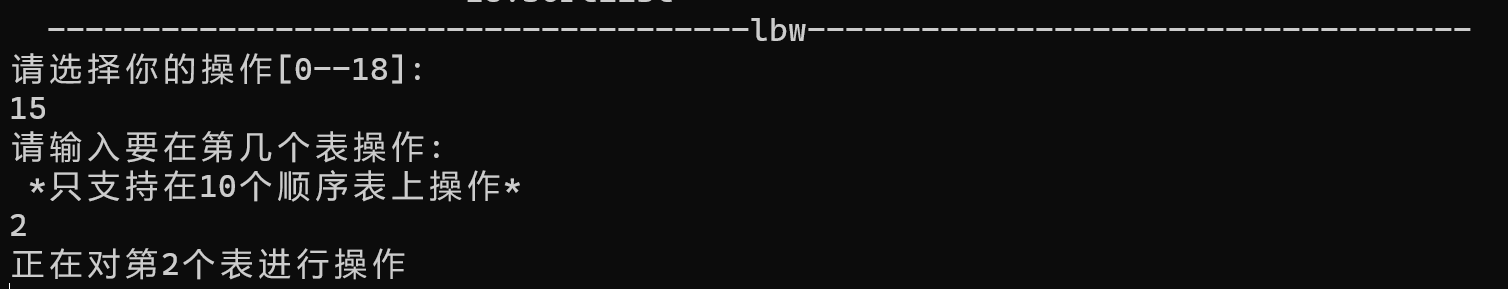
\includegraphics[width=1\linewidth]{images/多表切换.png}
			\includegraphics[width=1\linewidth]{images/多表操作成功.png}
			\includegraphics[width=1\linewidth]{images/多表操作结果.png}
			\caption{多线性表管理}
			\label{fig1-37}
		\end{figure}
	\end{enumerate}
\subsection{实验小结}
通过本次实验,我加深了对链式存储的线性表的理解,并掌握了如何运用单链表解决实际问题。
通过本次实验,我学到了:
\begin{enumerate}
	\item 单链表的定义
    \item 单链表的基本操作算法
	\item 链式存储线性表的定义
    \item 链式存储线性表的基本操作算法
    \item 链式存储线性表的管理表的定义
    \item 链式存储线性表的管理表的基本操作算法
    \item 单链表的实际应用
\end{enumerate}
通过本次实验,我认为我还有如下不足之处:
\begin{enumerate}
	\item 对单链表的指针操作不太熟练
    \item 不太明确线性表的实际应用
\end{enumerate}
\newpage

\section{基于二叉链表的二叉树实现}


\subsection{问题描述}

本实验实现了二叉树的二叉链表存储,构造一个具有菜单功能的演示系统,实现了二叉树的初始化、清空、求二叉树的深度等14种基本功能和全部的5种附加功能,还实现了多二叉树管理。

\subsection{系统设计}
基于二叉树的定义:二叉树是一种每个结点至多只有两个子树(即二叉树的每个结点的度不大于 2),并且二叉树的子树有左右之分,其次序不能任意颠倒。
本次实验采用树的链式存储方式,实现了树的基本的功能,比如增添、删除、查找等。同时,还在此基础上添加了一些高级功能,比如翻转、求最大路径和、求LCA等。该程序还使用语言文字提示,降低了程序的使用难度。

本实验涉及的头文件以及相关常量定义如下:
\begin{lstlisting}[title = 相关常量定义][frame=leftline,topline,rightline, bottomline]
/* Linear Table On Sequence Structure */
#include <stdio.h>
#include <malloc.h>
#include <stdlib.h>
#include <stack>
#include <queue>
#include <stdlib.h>

// 定义每个节点的打印宽度为 5
#define NODE_WIDTH 5

// 定义每个节点的占位符为 _
#define NODE_PLACEHOLDER '_'

/*---------page 10 on textbook ---------*/
#define TRUE 1//定义真值 
#define FALSE 0//定制假值 
#define OK 1//程序正常运行 
#define ERROR 0//程序运行出错 
#define INFEASTABLE -1//输入或输出不合法 
#define OVERFLOW -2//数值溢出 
#define MAX_NUM 10//最大个数 
#define LIST_INIT_SIZE 100//最大尺寸 
#define LISTINCRE MENT  10//最大增加量 

typedef int status;//定义所有状态码和返回值的类型为int
typedef char TElemType;//数据元素类型定义
status definition[1000]={0}; //定义并初始化关键字哈希表 
\end{lstlisting}
本系统的数据结构有两种:二叉树和二叉树的管理表。其具体定义如下。
\begin{lstlisting}[title = 相关数据结构定义][frame=leftline,topline,rightline, bottomline]
// 定义二叉树的节点结构体
typedef struct BiTNode{
	int key;  // 用 key 作为标记,便于查找节点
	TElemType data;  // char 类型数据域
	struct BiTNode *lchild, *rchild;  
	// 定义二叉链表的左孩子指针与右孩子指针
} BiTNode, *BiTree;  // BiTNode 类型指针 BiTree

// 定义一个结构体,用于保存二叉树和树的名称
typedef struct {
	BiTree T;  // 创建二叉树用的指针 T
	char name[20];  // 用于保存树的名称
} LElemType;

// 定义一个结构体,用于保存多个树进行操作
typedef struct {
	LElemType tree[20];  // 多个树进行操作
	int length;
	int listsize;
} SqList;
\end{lstlisting}

系统的总体架构:界面上采用简易菜单演示系统,在 while 循环中建立菜单
演示,op 代表用户选择的操作序号,程序将首先判断 op 的合法性,若合法则通
过 switch 函数进入功能的选择,进入相关功能函数执行相关操作,操作完成后
继续执行循环,直到用户输入 0 时,退出系统。

多线性表管理通过Choose函数实现,用户可以输入位序切换线性表,相关操作仅在当前树完成,而不会影响森林。
\begin{figure}[H]
	\centering
	\includegraphics[width=1\linewidth]{images/树的菜单设计.png}
	\caption{菜单演示系统}
	\label{fig2-1}
\end{figure}
\subsection{系统实现}
本程序在 Windows 11 系统下采用 Dev-C++ 进行编译调试,语言选择 C 语言
以下主要说明各个主要函数的实现思想,函数和系统实现的源代码放在附录中。

(\emph{本实验所有函数在实现功能之前会先对是否已有树进行判定,若树不存在,则返回 INFEASIBLE,在各函数具体设计思路中不再叙述此条。})


\begin{enumerate}
	\item 创建二叉树\\
	函数名称是CreateBiTree(T,definition);初始条件是definition 给出二叉树T的定义,如带空子树的二叉树前序遍历序列、或前序+中序、或后序+中序;操作结果是按definition构造二叉树T;
	
	如果二叉树已存在,返回不可行。检查关键字是否重复,若重复返回错误,否则调用递归函数create。
	递归函数通过definition数组检查输入的结点是否是空结点,若是则返回,否则创建并插入结点,再递归地创建左子树和右子树。
	
	\emph{复杂度:时间复杂度 T(n) = O(1)}
	\item 清空二叉树\\
	函数名称是ClearBiTree (T);初始条件是二叉树T存在;操作结果是将二叉树T清空;
	
	如果二叉树不存在,返回不可行。遇到空结点返回,递归地遍历左子树和右子树后释放结点空间。
	
	\emph{复杂度:时间复杂度 T(n) = O(n)}
	\item 销毁二叉树\\
	函数名称是DestroyBiTree(T);初始条件是二叉树T已存在;操作结果是销毁二叉树T;
	
	与清空操作类似,如果二叉树不存在,返回不可行。遇到空结点返回,递归地遍历左子树和右子树后释放结点空间。此外,不同于清空,我们还需要对头结点进行清除操作
	
\emph{复杂度:时间复杂度 T(n) = O(n)}
	\item 判定空二叉树\\
	函数名称是BiTreeEmpty(T);初始条件是二叉树T存在;操作结果是若T为空二叉树则返回TRUE,否则返回FALSE;
	
	仅需要判断头结点指针是否为空即可,T指向NULL则返回TRUE,不为空则返回FALSE。
	
	\emph{复杂度:时间复杂度 T(n) = O(1)}
	\item 求二叉树的深度\\
	函数名称是BiTreeDepth(T);初始条件是二叉树T存在;操作结果是返回T的深度;
	
	遇到空结点返回,使用递归方式计算左右子树的深度,然后取较大值加1作为当前树的深度。
	
	\emph{复杂度:时间复杂度 T(n) = O(n)}
	\item 查找结点\\
	函数名称是LocateNode(T,e);初始条件是二叉树T已存在,e是和T中结点关键字类型相同的给定值;操作结果是返回查找到的结点指针,如无关键字为e的结点,返回NULL;
	
	该函数的返回值为指针类型,在查找过程中基于关键字的唯一性,所以通过比较语句发现关键字相同的结点即可把当前遍历的结点作为返回值返回,在循环外返回空指针,表示遍历过程如果没有
	正常return,就说明树中没有对应的结点,返回空指针表示查找失败。
	
	\emph{复杂度:时间复杂度 T(n) = O(n)}
	
	\item 结点赋值\\
	函数名称是Assign(T,e,value);初始条件是二叉树T已存在,e是和T中结点关键字类型相同的给定值;操作结果是关键字为e的结点赋值为value;
	
	首先检查关键字是否重复,然后查找结点。如果结点关键字重复或结点未找到,返回错误,
	否则把找到的结点的关键字和名称赋值成用户输入的值。
	
	\emph{复杂度:时间复杂度 T(n) = O(n)}
	\item 获取兄弟结点\\
	函数名称是GetSibling(T,e);初始条件是二叉树T存在,e是和T中结点关键字类型相同的给定值;操作结果是返回关键字为e的结点的(左或右)兄弟结点指针。若关键字为e的结点无兄弟,则返回NULL;
	
	首先检查传入的结点是否是指定结点的双亲结点,如果是,返回其兄弟结点。如果结点为空,返回。否则递归地查找左子树和右子树。
	
	\emph{复杂度:时间复杂度 T(n) = O(n)}
	\item 插入结点\\
	函数名称是InsertNode(T,e,LR,c);初始条件是二叉树T存在,e是和T中结点关键字类型相同的给定值,LR为0或1,c是待插入结点;操作结果是根据LR为0或者1,插入结点c到T中,作为关键字为e的结点的左或右孩子结点,结点e的原有左子树或右子树则为结点c的右子树;
	
	首先检查关键字是否重复,然后查找结点。如果结点关键字重复或结点未找到,返回错误。再根据插入方向LR的不同,将子树c插入到父节点p的相应位置。如果插入方向为左子树,则先将p的左子树作为c的右子树,然后将c作为p的新左子树;如果插入方向为右子树,则先将p的右子树作为c的右子树,然后将c作为p的新右子树。
	
	\emph{复杂度:时间复杂度 T(n) = O(n)}
	\item 删除结点\\
	函数名称是DeleteNode(T,e);初始条件是二叉树T存在,e是和T中结点关键字类型相同的给定值。操作结果是删除T中关键字为e的结点;同时,如果关键字为e的结点度为0,删除即可;如关键字为e的结点度为1,用关键字为e的结点孩子代替被删除的e位置;如关键字为e的结点度为2,用e的左孩子代替被删除的e位置,e的右子树作为e的左子树中最右结点的右子树;
	
	首先检查关键字是否重复,然后根据删除方向LR的不同,先将父节点p的相应子树存储到临时变量T1中,再将父节点p的相应子树指针置为NULL,最后调用DestroyBiTree函数释放临时变量T1所指向的子树的内存空间。如果双亲进度结点未找到且删除的是根结点,直接清空二叉树。若销毁子树操作成功,则返回OK;否则返回ERROR。
	
	\emph{复杂度:时间复杂度 T(n) = O(n)}
	\item 先序遍历\\
	函数名称是PreOrderTraverse(T,Visit);初始条件是二叉树T存在;操作结果:先序遍历,对每个结点调用函数Visit一次且一次。
	
	首先访问当前结点,在递归访问左子树和右子树。
	
	\emph{复杂度:时间复杂度 T(n) = O(n)}
	\item 中序遍历\\
	函数名称是InOrderTraverse(T,Visit);初始条件是二叉树T存在;操作结果:中序遍历,对每个结点调用函数Visit一次且一次,
	
	首先递归访问左子树,然后访问当前结点,再递归地访问右子树。
	
	\emph{复杂度:时间复杂度 T(n) = O(n)}
	\item 后序遍历\\
	函数名称是PostOrderTraverse(T,Visit);初始条件是二叉树T存在;操作结果:后序遍历,对每个结点调用函数Visit一次且一次,
	
	首先递归访问左子树和右子树,再访问当前结点。
	
	\emph{复杂度:时间复杂度 T(n) = O(n)}
	\item 按层遍历\\
	函数名称是LevelOrderTraverse(T,Visit);初始条件是二叉树T存在;
	
	采用广度优先搜索遍历二叉树。首先新建队列并将根结点入队,然后逐个访问队首元素,把队首元素的未入队子结点入队,弹出队首元素,直到队列为空。
	
	\emph{复杂度:时间复杂度 T(n) = O(n)}
	\item 翻转二叉树\\
	函数名称是InvertTree(T),初始条件是线性表L已存在;操作结果是将T翻转,使其所有节点的左右节点互换;
	
	首先交换传入结点的两个子结点,如果是空结点则返回,然后递归地翻转左子树和右子树。
	
	\emph{复杂度:时间复杂度 T(n) = O(n)}
	\begin{figure}[H]
		\centering
		\begin{minipage}{0.7\linewidth}
			\centering
			\includegraphics[width=0.9\linewidth]{images/翻转树.png}
		\end{minipage}
		\caption{翻转二叉树}
		\label{fig2-2}
	\end{figure}
	\item 最大路径和\\
	函数名称是MaxPathSum(T),初始条件是二叉树T存在;操作结果是返回根节点到叶子结点的最大路径;
	
	遇到空结点返回,否则递归地计算左子树和右子树的最大路径和,取最大的一个的值加上传入顶点的权值后返回。

    \emph{复杂度:时间复杂度 T(n) = O(n)}
    	\begin{figure}[H]
    	\centering
    	\begin{minipage}{0.8\linewidth}
    		\centering
    		\includegraphics[width=0.9\linewidth]{images/最大路径和.png}
    	\end{minipage}
    	\caption{最大路径和}
    	\label{fig2-3}
    \end{figure}
	\item 最近公共祖先\\
	函数名称是LowestCommonAncestor(T,e1,e2);初始条件是二叉树T存在;操作结果是该二叉树中e1节点和e2节点的最近公共祖先;
	
	首先查找结点,如果两个结点中有未找到的,返回错误。然后调用递归函数LCA,LCA中序遍历二叉树,从访问了一个结点开始计数,
	求这时开始到访问到第二个结点时到达的层数最小的结点,这个结点就是最近公共祖先。

	\emph{复杂度:时间复杂度 T(n) = O(n)}
		\begin{figure}[H]
		\centering
		\begin{minipage}{0.7\linewidth}
			\centering
			\includegraphics[width=0.9\linewidth]{images/lca.png}
		\end{minipage}
		\caption{最近公共祖先}
		\label{fig2-4}
	\end{figure}
	\item 线性表的文件操作\\
	如果线性表不存在,返回不可行。打开只写文件,调用递归函数 save, 如果传入结点为空,返回。写入传入的二叉树结点,然后递归地写入左子树和右子树。最后清空二叉树。接着创建
	新二叉树,以只读模式打开刚才保存的文件,调用递归函数 load, 新建结点,
	读入数据。插入新二叉树,然后递归地读取左子树和右子树。

	\emph{复杂度:时间复杂度 T(n) = O(1)}
\begin{figure}[H]
	\centering
	\begin{minipage}{0.7\linewidth}
		\centering
		\includegraphics[width=0.9\linewidth]{images/文件保存.png}
	\end{minipage}
	\caption{文件保存}
	\label{fig2-5}
\end{figure}

\begin{figure}[H]
	\centering
	\begin{minipage}{0.7\linewidth}
		\centering
		\includegraphics[width=0.9\linewidth]{images/文件读取.png}
	\end{minipage}
	\caption{文件读取}
	\label{fig2-6}
\end{figure}
%\newpage
\item 实现多个树管理:设计相应的数据结构管理多个树的查找、添加、移除等功能。

与多链表的管理类似,本实验设计一个结构体,其中定义了一个结构体数组,本质上是通过数组存储多个树以此实现多个树的管理,针对数组中每个树的管理
和上述基础功能对单个树的操作基本一致,不同在于,我们需要实现不同树的切换,即找寻并切换至目标树进行管理。

在设计过程中每一个树都有一个name数组对链表以及对应的位序,因此,我们可以更改序号来切换不同链表,若没有找到目标或者查找的序号超过森林的最大数量,则返返回ERROR。

复杂度:时间复杂度 T(n) = O(1)
\begin{figure}[H]
	\centering
	\begin{minipage}{0.8\linewidth}
		\centering
		\includegraphics[width=0.9\linewidth]{images/多树管理.png}
	\end{minipage}
	\caption{多树管理的实现}
	\label{fig2-7}
\end{figure}
\newpage

\end{enumerate}
\subsection{系统测试}
以下主要说明针对各个函数正常和异常的测试用例及测试结果。

\emph{1 1 a  2 2 b   3 3 c  6 4 d  7 5 e  0 0 null}
\begin{enumerate}
	\item 创建二叉树\\
	以前序的方式输入输入二叉树A,\emph{1 1 a  2 2 b   3 3 c  6 4 d  7 5 e  0 0 null},输出结果如下图:
\begin{figure}[H]
	\centering
	\includegraphics[width=1\linewidth]{images/创建二叉树.png}
	\caption{创建二叉树}
	\label{fig2-8}
\end{figure}
	\item 清空二叉树\\
	若二叉树不存在,输出结果如下图:
	\begin{figure}[H]
		\centering
		\includegraphics[width=1\linewidth]{images/二叉树清空失败.png}
		\caption{二叉树清空失败}
		\label{fig2-9}
	\end{figure}

	若二叉树存在,输出结果如下图:
	\begin{figure}[H]
		\centering
		\includegraphics[width=1\linewidth]{images/二叉树清空成功.png}
		\caption{二叉树清空成功}
		\label{fig2-10}
	\end{figure}
	\item 求二叉树的深度\\
	若二叉树不存在,输出结果如下图:
	\begin{figure}[H]
		\centering
		\includegraphics[width=1\linewidth]{images/求深度失败.png}
		\caption{二叉树求深度失败}
		\label{fig2-11}
	\end{figure}

		若二叉树不存在,输出结果如下图:
	\begin{figure}[H]
		\centering
		\includegraphics[width=1\linewidth]{images/求深度成功.png}
		\caption{二叉树求深度成功}
		\label{fig2-12}
	\end{figure}
	\item 查找结点\\
	输入二叉树A,查找关键字为9的节点,输出结果如下图:
		\begin{figure}[H]
		\centering
		\includegraphics[width=1\linewidth]{images/查找失败.png}
		\caption{查找结点失败}
		\label{fig2-13}
	\end{figure}

	输入二叉树A,查找关键字为1的节点,输出结果如下图:
	\begin{figure}[H]
		\centering
		\includegraphics[width=1\linewidth]{images/查找节点成功.png}
		\caption{查找结点成功}
		\label{fig2-14}
	\end{figure}
	\item 结点赋值\\
	输入二叉树A,将关键字为1的节点赋值为关键字为4,节点名称赋值为f,输出结果如下图:
	\begin{figure}[H]
		\centering
		\includegraphics[width=1\linewidth]{images/赋值失败.png}
		\caption{结点赋值成功}
		\label{fig2-15}
	\end{figure}
	输入二叉树A,将关键字为1的节点赋值为关键字为4,节点名称赋值为f,输出结果如下图:
	\begin{figure}[H]
		\centering
		\includegraphics[width=1\linewidth]{images/赋值成功.png}
		\caption{结点赋值成功}
		\label{fig2-16}
	\end{figure}
	\item 获取兄弟结点\\
	输入二叉树A,获取关键字为3节点的兄弟节点,输出结果如下图:
	\begin{figure}[H]
		\centering
		\includegraphics[width=1\linewidth]{images/查找兄弟成功.png}
		\caption{获取兄弟结点成功}
		\label{fig2-17}
	\end{figure}

	\item 插入结点\\
	输入二叉树A,插入节点8 g到关键字为2节点的右边,输出结果如下图:
		\begin{figure}[H]
		\centering
		\includegraphics[width=1\linewidth]{images/插入节点成功.png}
		\caption{插入节点成功}
		\label{fig2-18}
	\end{figure}
	
	\item 删除结点\\
	输入二叉树A,删除关键字为2的节点,输出结果如下图:
	\begin{figure}[H]
		\centering
		\includegraphics[width=0.8\linewidth]{images/删除节点成功.png}
		\caption{删除结点成功}
		\label{fig2-19}
	\end{figure}
	\item 先序遍历\\
		输入二叉树A,进行先序遍历,输出结果如下图:
	\begin{figure}[H]
		\centering
		\includegraphics[width=0.9\linewidth]{images/先序遍历.png}
		\caption{先序遍历}
		\label{fig2-20}
  \end{figure}
	\item 中序遍历\\
		输入二叉树A,进行先序遍历,输出结果如下图:
\begin{figure}[H]
	\centering
	\includegraphics[width=0.9\linewidth]{images/中序遍历.png}
	\caption{中序遍历}
	\label{fig2-21}
  \end{figure}
	\item 后序遍历\\
			输入二叉树A,进行先序遍历,输出结果如下图:
	\begin{figure}[H]
		\centering
		\includegraphics[width=0.9\linewidth]{images/后序遍历.png}
		\caption{后序遍历}
		\label{fig2-22}
	  \end{figure}
	\item 层序遍历\\
	输入二叉树A,进行先序遍历,输出结果如下图:
	\begin{figure}[H]
		\centering
		\includegraphics[width=0.9\linewidth]{images/层序遍历.png}
		\caption{层序遍历}
		\label{fig2-23}
	  \end{figure}
	\item 翻转二叉树\\
	输入二叉树A,输出结果如下图:
	\begin{figure}[H]
		\centering
		\includegraphics[width=0.9\linewidth]{images/翻转树成功.png}
		\caption{翻转二叉树}
		\label{fig2-24}
	  \end{figure}
	\item 最大路径和\\
	输入二叉树A,输出结果如下图:
	\begin{figure}[H]
		\centering
		\includegraphics[width=0.9\linewidth]{images/求最大路径和成功.png}
		\caption{最大路径和}
		\label{fig2-25}
	\end{figure}
	\item 最近公共祖先\\
		输入二叉树A,输出结果如下图:
		\begin{figure}[H]
			\centering
			\includegraphics[width=0.9\linewidth]{images/求lca成功.png}
			\caption{最近公共祖先}
			\label{fig2-26}
		\end{figure}
		
\item 二叉树的文件操作\\
文件保存:将以上二叉树A保存为test.txt文件,文件内容如下:
\begin{figure}[H]
	\centering
	\includegraphics[width=0.9\linewidth]{images/二叉树文件保存.png}
	\caption{文件保存}
	\label{fig2-27}
\end{figure}

文件读取:初始化二叉树后,我们读入test.txt文件,输出结果如下图:
\begin{figure}[H]
	\centering
	\includegraphics[width=0.9\linewidth]{images/二叉树读取成功.png}
	\caption{文件读取}
	\label{fig2-28}
\end{figure}

\item 多线性表管理\\
对第一个树,读取test.txt文件,切换到到第2个树并初始化。此时第一个树不为空树,而第二个表为空树,从而说明多线性表操作的独立性与正确性:
\begin{figure}[H]
	\centering
	\includegraphics[width=1\linewidth]{images/多树操作前.png}
	\includegraphics[width=1\linewidth]{images/多树切换.png}
	\includegraphics[width=1\linewidth]{images/多树操作成功.png}
	\caption{多树管理}
	\label{fig2-29}
\end{figure}

\end{enumerate}
\subsection{实验小结}
通过本次实验,我加深了对二叉链表存储的二叉树的理解,并掌握了如何运用二叉树解决实际问题。
通过本次实验,我学到了:
\begin{enumerate}
	\item 二叉链表的定义
    \item 二叉链表的基本操作算法
	\item 二叉链表存储的二叉树的定义
    \item 二叉链表存储的二叉树的基本操作算法
    \item 二叉树的管理表的定义
    \item 二叉树的管理表的基本操作算法
    \item 二叉树的实际应用
\end{enumerate}
通过本次实验,我认为我还有如下不足之处:
\begin{enumerate}
	\item 对其他结构存储的二叉树操作不够熟练
    \item 对二叉树的复杂操作不够熟练
\end{enumerate}
\newpage


\section{课程的收获和建议}


\subsection{基于顺序存储结构的线性表实现}

我的收获:
\begin{enumerate}
	\item 加深了对顺序表存储的线性表的理解
    \item 掌握了如何运用线性表解决实际问题
    \item 学到了顺序表的定义
    \item 学到了顺序表的基本操作算法
\end{enumerate}
我的建议:
\begin{enumerate}
	\item 增加一些有实际应用背景的实验内容
    \item 减少一些过于基础的实验内容
\end{enumerate}

\subsection{基于链式存储结构的线性表实现}

我的收获:
\begin{enumerate}
	\item 加深了对链式存储的线性表的理解
    \item 掌握了如何运用线性表解决实际问题
    \item 学到了单链表的定义
    \item 学到了单链表的基本操作算法
    \item 学到了单链表的管理表的定义
    \item 学到了单链表的管理表的基本操作算法
\end{enumerate}
我的建议:
\begin{enumerate}
	\item 增加一些有实际应用背景的实验内容
    \item 增加一些有关next指针操作的实验内容
    \item 增加一些有关静态链表操作的实验内容
    \item 减少一些过于基础的实验内容
\end{enumerate}

\subsection{基于二叉链表的二叉树实现}

我的收获:
\begin{enumerate}
	\item 加深了对二叉链表存储的二叉树的理解
    \item 掌握了如何运用二叉树解决实际问题
    \item 学到了二叉链表的定义
    \item 学到了二叉链表的基本操作算法
    \item 学到了二叉树的管理表的定义
    \item 学到了二叉树的管理表的基本操作算法
\end{enumerate}
我的建议:
\begin{enumerate}
	\item 增加一些有实际应用背景的实验内容
    \item 增加一些以其它存储方式实现的二叉树的实验
    \item 增加有关堆,AVL树的操作内容
\end{enumerate}

\subsection{基于邻接表的图实现}

我的收获:
\begin{enumerate}
	\item 加深了对图的理解
    \item 掌握了如何图解决实际问题
    \item 学到了邻接表的定义
    \item 学到了邻接表的基本操作算法
    \item 学到了图的管理表的定义
    \item 学到了图的管理表的基本操作算法
\end{enumerate}
我的建议:
\begin{enumerate}
	\item 增加一些有实际应用背景的实验内容
    \item 增加除邻接表以外的存储图的实验
\end{enumerate}

\newpage
\section{参考文献}
\begin{enumerate}
	\item 严蔚敏等.数据结构(C语言版).清华大学出版社
    \item Larry Nyhoff. ADTs, Data Structures, and Problem Solving with C++. Second Edition,Calvin College,2005
    \item 严蔚敏等.数据结构题集(C语言版).清华大学出版社
\end{enumerate}
\newpage

\section{附录A 基于顺序存储结构线性表实现的源程序}
\begin{lstlisting}[title =相关定义,frame=none]
/* Linear Table On Sequence Structure */
#include <stdio.h>
#include <malloc.h>
#include <stdlib.h>

/*---------page 10 on textbook ---------*/
/* 定义常量 */
#define TRUE 1
#define FALSE 0
#define OK 1
#define ERROR 0
#define INFEASTABLE -1
#define OVERFLOW -2
#define MAX_NUM 10
/* 定义数据类型 */
typedef int status;
typedef int ElemType; //数据元素类型定义

/*-------page 22 on textbook -------*/
/* 定义顺序表结构体 */
#define LIST_INIT_SIZE 100
#define LISTINCREMENT  10
typedef struct{  //顺序表(顺序结构)的定义
	ElemType * elem;
	int length;
	int listsize;
}SqList;
/* 定义全局变量 */
FILE *fp;
/*-----page 19 on textbook ---------*/
/* 函数声明 */ 
status IntiaList(SqList &L);              
// 初始化顺序表
status DestroyList(SqList &L);             
// 销毁顺序表
status ClearList(SqList &L);               
// 清空顺序表
status ListEmpty(SqList L);                
// 判断顺序表是否为空
int ListLength(SqList L);                  
// 获取顺序表长度
status GetElem(SqList L,int i,ElemType *e); 
// 获取指定位置的元素
status LocateElem(SqList L, ElemType e, status(*compare)(ElemType,ElemType)); 
// 查找元素
status compare(ElemType a, ElemType b);     
// 比较元素
status PriorElem(SqList L,ElemType cur_e,ElemType *pre_e); 
// 获取指定元素的前一个元素
status NextElem(SqList L,ElemType cur_e,ElemType *next_e); 
// 获取指定元素的后一个元素
status ListInsert(SqList &L,int i,ElemType e); 
// 在指定位置插入元素
status ListDelete(SqList *L,int i,ElemType *e); 
// 删除指定位置的元素
status ListTrabverse(SqList L);             
// 遍历顺序表
status SaveList(SqList L, char *filename); 
// 将顺序表保存到文件
status LoadList(SqList *L, char *filename); 
// 从文件中加载顺序表
int countSubarray(SqList L, int k);         
// 计算顺序表中和为k的子数组个数
int maxSubArraySum(SqList L);               
// 求顺序表中连续子数组的最大和
int SortList(SqList &L); 
//排序顺序表 
int max(int a, int b) ; 
//求两个数中的最大值 
/*--------------------------------------------*/
\end{lstlisting}
\begin{lstlisting}[title =演示系统,frame=none]
int main(void){
	char filename[40];
	int op=1;
	int i;
	int i_num=1;
	SqList L[MAX_NUM];
	for(i=0;i<MAX_NUM;i++)
	{
		L[i].elem = NULL;
		L[i].listsize = 0;
		L[i].length = 0;
	}
	//上面的for循环是用来生成没有存储空间的线性表
	ElemType e, cur_e , pre_e, next_e;
	while(op){
		/**
		*利用最简单的printf来制作简易的菜单,可供选择;
		*简洁美观的菜单有助于平复测试时的心情!!!
		*/
		system("cls");	//用于清屏
		printf("\n\n");
		printf("      \t\t\tMenu for Linear Table On Sequence Structure \n");
		printf("  可在%d个顺序表进行多表操作,初始化请先操作功能15,默认在第一个表上操作\n", MAX_NUM);
		printf("  ------------------------------------------------------------------------------\n");
		printf("**\t\t\t1. IntiaList       7.  LocateElem\t\t\t**\n");
		printf("**\t\t\t2. DestroyList     8.  PriorElem\t\t\t**\n");
		printf("**\t\t\t3. ClearList       9.  NextElem \t\t\t**\n");
		printf("**\t\t\t4. ListEmpty       10. ListInsert\t\t\t**\n");
		printf("**\t\t\t5. ListLength      11. ListDelete\t\t\t**\n");
		printf("**\t\t\t6. GetElem         12. ListTrabverse\t\t\t**\n");
		printf("**\t\t\t13.SaveList	    14. LoadList\t\t\t**\n");
		printf("**\t\t\t0. Exit         				   \n");
		printf("**\t\t\t15.ChooseList(请先进行此选项以选择在哪个表上进行操作)\n");
		printf("**\t\t\t16.countSubarray           17.maxSubArraySum\n");
		printf("**\t\t\t18.SortList                                 \n");
		printf("  -------------------------------------lbw-----------------------------------\n");
		printf("请选择你的操作[0--18]:\n");
		scanf("%d",&op);//选择op的值,用于switch
		switch(op){
			case 1:
			//第一种情况是初始化线性表
			if(IntiaList(L[i_num])==OK)
			{
				
				printf("请输入要保存的线性表名称\n");
				scanf("%s", filename);
				printf("线性表创建成功\n");
			}
			else printf("线性表创建失败!\n");
			getchar();getchar();
			break;
			
			case 2:
			//第二种情况是用来销毁线性表
			if(L[i_num].elem == NULL)
			{
				printf("线性表不存在!\n");
				getchar();getchar();
				break;
			}
			if(DestroyList(L[i_num])==OK)
			{
				printf("销毁线性表成功!\n");
			}
			else printf("销毁线性表失败!\n");
			getchar();getchar();
			break;
			
			case 3:
			//用于重置线性表
			if(L[i_num].elem == NULL)
			{
				printf("线性表不存在!\n");
				getchar();getchar();
				break;
			}
			if(ClearList(L[i_num])==OK)
			{
				printf("线性表重置成功!\n");
			}
			else printf("线性表重置失败!\n");
			getchar();getchar();
			break;
			
			case 4:
			//判断是否为空
			if(L[i_num].elem == NULL)
			{
				printf("线性表不存在!\n");
				getchar();getchar();
				break;
			}
			if(ListEmpty(L[i_num])==TRUE)
			{
				printf("文件为空!\n");
			}
			else printf("线性表不是空表!\n");
			getchar();getchar();
			break;
			
			case 5:
			//得到线性表长度
			if(L[i_num].elem == NULL)
			{
				printf("线性表不存在!\n");
				getchar();getchar();
				break;
			}
			printf("线性表表长为%d\n",ListLength(L[i_num]));
			getchar();getchar();
			break;
			
			case 6:
			//得到某个元素
			if(L[i_num].elem == NULL)
			{
				printf("线性表不存在!\n");
				getchar();getchar();
				break;
			}
			printf("请输入要取结点的位置:\n");
			scanf("%d",&i);
			if(GetElem(L[i_num],i,&e)==OK)
			printf("第%d个结点的元素是:%d\n",i,e);
			else  printf("输入位置错误!\n");
			getchar();getchar();
			break;
			
			case 7:
			//确定元素位置,容易出错
			if(L[i_num].elem == NULL)
			{
				printf("线性表不存在!\n");
				getchar();getchar();
				break;
			}
			printf("请输入数据元素值:\n");
			scanf("%d",&e);
			if(i=LocateElem(L[i_num],e,compare))
			printf("%d元素位于第%d个位置!\n",e,i);
			else  printf("该元素不存在!\n");
			getchar();getchar();
			break;
			
			case 8:
			//求出前驱结点
			if(L[i_num].elem == NULL)
			{
				printf("线性表不存在!\n");
				getchar();getchar();
				break;
			}
			printf("请输入数据元素:\n");
			scanf("%d",&cur_e);
			PriorElem(L[i_num],cur_e,&pre_e);
			if(PriorElem(L[i_num],cur_e,&pre_e)==OK)
			printf("其前驱元素为:%d\n",pre_e);
			else if(PriorElem(L[i_num],cur_e,&pre_e)==OVERFLOW)
			printf("顺序表中没有该元素!\n");
			else  printf("其不存在前驱元素!\n");
			getchar();getchar();
			break;
			
			case 9:
			//求出后置节点
			if(L[i_num].elem == NULL)
			{
				printf("线性表不存在!\n");
				getchar();getchar();
				break;
			}
			printf("请输入数据元素:\n");
			scanf("%d",&cur_e);
			if(NextElem(L[i_num],cur_e,&next_e)==OK)
			printf("其后继元素为:%d\n",next_e);
			else if(NextElem(L[i_num],cur_e,&pre_e)==FALSE)
			printf("其不存在后继元素!\n");
			else
			{printf("顺序表中没有该元素!\n");}
			getchar();getchar();
			break;
			
			case 10:
			//插入元素
			if(L[i_num].elem == NULL)
			{
				printf("线性表不存在!\n");
				getchar();getchar();
				break;
			}
			printf("请输入您要插入的数据元素:\n");
			scanf("%d",&e);
			printf("请输入您要插入的数据元素的位置:\n");
			scanf("%d",&i);
			if(ListInsert(L[i_num],i,e)==OK)
			printf("插入数据元素成功!\n");
			else
			printf("插入数据元素失败!\n");
			getchar();getchar();
			break;
			
			case 11:
			//删除元素
			if(L[i_num].elem == NULL)
			{
				printf("线性表不存在!\n");
				getchar();getchar();
				break;
			}
			printf("请输入您要删除的数据元素的位置:\n");
			scanf("%d",&i);
			if(ListDelete(&L[i_num],i,&e)==OK)
			printf("删除数据元素成功!\n");
			else
			printf("删除数据元素失败!\n");
			getchar();getchar();
			break;
			case 12:
			//遍历线性表中的元素
			if(L[i_num].elem == NULL)
			{
				printf("线性表不存在!\n");
				getchar();getchar();
				break;
			}
			if(!ListTrabverse(L[i_num])) printf("线性表是空表!\n");
			getchar();getchar();
			break;
			
			case 13:
			//保存文件
			if(L[i_num].elem == NULL)
			{
				printf("线性表不存在!\n");
				getchar();getchar();
				break;
			}
			if(SaveList(L[i_num], filename)==OK)
			printf("文件保存成功\n文件名为%s\n",filename);
			break;
			
			case 14:
			//加载文件,需要输入需要加载的名称
			printf("请输入要加载的文件名:\n ");
			scanf("%s", filename);
			if(LoadList(&L[i_num], filename)==OK)
			{
				printf("文件加载成功\n");
			}
			break;
			case 15:
			//选择在哪个表进行操作
			printf("请输入要在第几个表操作:\n ");
			printf("*只支持在%d个顺序表上操作*\n",MAX_NUM);
			scanf("%d",&i_num);
			printf("正在对第%d个表进行操作\n",i_num);
			if((i_num<1)||(i_num>10))
			{
				printf("请选择正确范围!\n");
				i_num=1;
			}
			getchar(); getchar();
			break;
			break;
			case 16:
			//和为k的子数组个数
			int ret;
			int k; 
			printf("请输入k\n ");
			scanf("%d",&k);
			ret= countSubarray(L[i_num], k);
			if(ret==ERROR){
				printf("线性表不存在");
				getchar();getchar();
				break;
			}
			printf("和为%d的子数组个数为%d\n",k,ret);
			getchar();getchar();
			break;
			case 17:
			//最大连续子数组和 
			ret= maxSubArraySum(L[i_num]);
			if(ret==ERROR){
				printf("线性表不存在");
				getchar();getchar();
				break;
			}
			printf("最大连续子数组和为%d\n",ret);
			getchar();getchar();
			break;
			case 18:
			//线性表排序 
			ret=SortList(L[i_num]); 
			if(ret==ERROR){
				printf("线性表不存在");
				getchar();getchar();
				break;
			}
			printf("已完成排序\n");
			getchar();getchar();
			break;
			case 0:
			//退出菜单,退出整个程序
			break;
		}//end of switch
	}//end of while
	printf("欢迎下次再使用本辣鸡系统!\n");
}//end of main()
/*--------page 23 on textbook --------------------*/
\end{lstlisting}
\begin{lstlisting}[title =函数实现,frame=none]
/***************************************************************
*函数名称:IntiaList
*函数功能:构造一个空的线性表
*注释:初始条件是线性表L不存在已存在;操作结果是构造一个空的线性表。
*返回值类型:status类型
****************************************************************/
status IntiaList(SqList &L){
	L.elem = (ElemType *)malloc( LIST_INIT_SIZE * sizeof (ElemType));
	if(!L.elem) exit(OVERFLOW);//如果空间不足,创建失败
	L.length=0;
	L.listsize=LIST_INIT_SIZE;
	return OK;
}


/***************************************************************
*函数名称:DestoryList
*函数功能:销毁线性表
*注释:初始条件是线性表L已存在;操作结果是销毁线性表L
*返回值类型:status类型
****************************************************************/
status DestroyList(SqList &L)
{
	if(L.elem)
	free(L.elem);
	L.elem = NULL;
	L.length = 0;
	L.listsize = 0;
	return OK;
}


/***************************************************************
*函数名称:ClearList
*函数功能:重置顺序表
*注释:初始条件是线性表L已存在;操作结果是将L重置为空表。
*返回值类型:status类型
****************************************************************/
status ClearList(SqList &L)
{
	L.length=0;
	return OK;
}



/***************************************************************
*函数名称:ListEmpty
*函数功能:判断线性表是否为空
*注释:初始条件是线性表L已存在;操作结果是若L为空表则返回TRUE,否则返回FALSE。
*返回值类型:status类型
****************************************************************/
status ListEmpty(SqList L)
{
	if(L.length==0)
	{
		return TRUE;
	}
	return FALSE;
	
}


/***************************************************************
*函数名称:ListLength
*函数功能:求线性表的表长
*注释:初始条件是线性表已存在;操作结果是返回L中数据元素的个数。
*返回值类型:int类型
****************************************************************/
int ListLength(SqList L)
{
	return L.length;
}


/***************************************************************
*函数名称:GetElem
*函数功能:得到某一个元素的值
*注释:初始条件是线性表已存在,1≤i≤ListLength(L);操作结果是用e返回L中第i个数据元素的值
*返回值类型:status类型
****************************************************************/
status GetElem(SqList L,int i,ElemType *e)
{
	if(i<1||i>L.length)
	{
		return ERROR;
	}
	*e = L.elem[i-1];
	return OK;
}



/***************************************************************
*函数名称:LocateElem
*函数功能:查找元素
*注释:初始条件是线性表已存在;操作结果是返回L中第1个与e满足关系compare()
关系的数据元素的位序,若这样的数据元素不存在,则返回值为0。
*返回值类型:status类型
****************************************************************/
status LocateElem(SqList L,ElemType e,status(*compare)(ElemType,ElemType))
{
	int i;
	for(i=0;i<L.length;i++)
	{
		if(compare(L.elem[i],e))
		return ++i;
	}
	return 0;
}


/***************************************************************
*函数名称:compare
*函数功能:比较大小,服务于LocateList函数
*注释:输入两个ElemType类型的值
*返回值类型:status类型
****************************************************************/
status compare(ElemType a, ElemType b)
{
	if(a == b)
	return TRUE;
	else  return FALSE;
}




/***************************************************************
*函数名称:PriorElem
*函数功能:求元素的前驱
*注释:初始条件是线性表L已存在;操作结果是若cur_e是L的数据元素,且不是第一个,
则用pre_e返回它的前驱,否则操作失败,pre_e无定义。
*返回值类型:status类型
****************************************************************/
status PriorElem(SqList L,ElemType cur_e,ElemType *pre_e)
{
	int i;
	for(i=0;i<L.length;i++)
	{
		if(L.elem[i]==cur_e && i==0)
		{
			return ERROR;
		}
		else if(L.elem[i]== cur_e)
		{
			*pre_e = L.elem[i-1];
			return OK;
		}
	}
	return OVERFLOW;
}





/***************************************************************
*函数名称:NextElem
*函数功能:求后继节点
*输入输出:初始条件是线性表L已存在;操作结果是若cur_e是L的数据元素,且不是最后一个,
则用next_e返回它的后继,否则操作失败,next_e无定义。
*返回值类型:status类型
****************************************************************/
status NextElem(SqList L,ElemType cur_e,ElemType *next_e)
{
	int i;
	for(i=0;i<(L.length-1);i++)
	{
		if(L.elem[i]==cur_e)
		{
			*next_e = L.elem[i+1];
			return OK;
		}
		
	}
	if(i==L.length-1 && (L.elem[i]!=cur_e)) return OVERFLOW;
	else return FALSE;
}



/***************************************************************
*函数名称:ListInsert
*函数功能:插入元素
*注释:初始条件是线性表L已存在且非空,1≤i≤ListLength(L)+1;
*      操作结果是在L的第i个位置之前插入新的数据元素e
*返回值类型:status类型
****************************************************************/
status ListInsert(SqList &L,int i,ElemType e)
{
	int *p,*q,*newbase;
	if(i<1||i>L.length+1)
	{
		printf("插入位置不正确!\n");
		return ERROR;
	}
	
	if(L.length>=L.listsize){
		newbase = (ElemType *)realloc(L.elem,(L.listsize + LISTINCREMENT)*sizeof(ElemType));
		if(!newbase) exit(OVERFLOW);
		L.elem = newbase;
		L.listsize += LISTINCREMENT;
	}
	q = &(L.elem[i-1]);
	for(p=&(L.elem[L.length-1]);p>=q;--p) *(p+1) = *p;
	*q=e;
	++L.length;
	return OK;
	
}
//这是课本上面的关于插入算法的实现





/***************************************************************
*函数名称:ListDelete
*函数功能:删除元素
*注释:初始条件是线性表L已存在且非空,1≤i≤ListLength(L);
*      操作结果:删除L的第i个数据元素,用e返回其值。
*返回值类型:status类型
****************************************************************/
status ListDelete(SqList *L,int i,ElemType *e)
{
	if(i<1||i>L->length)
	return ERROR;//删除的位数不正确
	int j;
	*e=L->elem[i-1];
	for (j = i - 1; j<L->length; j++)
	L->elem[j] = L->elem[j + 1];
	L->length--;
	return OK;
}




/***************************************************************
*函数名称:ListTrabverse
*函数功能:遍历顺序表
*注释:输出顺序表的值
*返回值类型:status类型
****************************************************************/
status ListTrabverse(SqList L){
	int i;
	printf("\n-----------all elements -----------------------\n");
	for(i=0;i<L.length;i++) printf("%d ",L.elem[i]);
	printf("\n------------------ end ------------------------\n");
	return L.length;
}






/***************************************************************
*函数名称:SaveList
*函数功能:保存线性表
*注释:将线性表保存,参考附录B,其中关于写入元素个数和长度的问题理解不够清楚
*返回值类型:
****************************************************************/
status SaveList(SqList L, char* filename)
{
	int i = 0;
	if ((fp = fopen(filename, "w")) == NULL)
	{
		printf("文件保存失败\n");
		return ERROR;
	}
	fprintf(fp, "%d ", L.length);//保存的时候,也将L的长度保存到了文件
	fprintf(fp, "%d ", L.listsize);//将每个元素的大小也保存到了文件里
	while (i < L.length)
	fprintf(fp, "%d ", L.elem[i++]);//利用循环,将元素依次存进去
	fclose(fp);//关闭文件
	return OK;
}







/***************************************************************
*函数名称:LoadList
*函数功能:加载文件
*注释:加载文件,以便功能的测试,文件名要正确
*返回值类型:status类型
****************************************************************/
status LoadList(SqList *L, char *filename)
{
	int i = 0;
	if ((fp = fopen(filename, "r")) == NULL)
	{
		printf("文件加载失败\n");
		return ERROR;
	} 
	fscanf(fp, "%d ", &L->length);
	fscanf(fp, "%d ", &L->listsize);
	L->elem = (ElemType *)malloc(L->listsize * sizeof(ElemType));
	if (!L->elem) exit(OVERFLOW);
	while (i < L->length)
	fscanf(fp, "%d ", &L->elem[i++]);//利用循环,依次读出文件中的内容
	fclose(fp);
	return OK;
}


/***************************************************************
函数名称:countSubarray
函数功能:计算线性表中和为k的子数组个数
参数:SqList L - 线性表int k - 和值
返回值类型:int - 符合条件的子数组个数
****************************************************************/
int countSubarray(SqList L, int k) {
	if(L.length==0){
		return  ERROR;
	}
	int count = 0;
	int sum = 0;
	for (int i = 1; i <= L.length; i++) {  // 枚举子数组的起始位置
		sum = 0;
		for (int j = i; j <= L.length; j++) {  // 枚举子数组的终止位置
			sum += L.elem[j-1];
			if (sum == k) {
				count++;
			}
		}
	}
	return count;
}


/***************************************************************
函数名称:maxSubArraySum
函数功能:计算线性表的最大子序和
参数:SqList L - 线性表
返回值类型:int - 线性表的最大子序和
****************************************************************/
int maxSubArraySum(SqList L) {
	if(L.length==0){
		return  ERROR;
	}
	int max_so_far = L.elem[0];
	int curr_max = L.elem[0];
	int n = L.length;
	for (int i = 1; i < n; i++) {
		curr_max = max(L.elem[i], curr_max + L.elem[i]);
		max_so_far = max(max_so_far, curr_max);
	}
	return max_so_far;
}

/***************************************************************
函数名称:SortList
函数功能:对线性表进行选择排序
参数:SqList &L - 线性表的引用
返回值类型:int - 返回值为排序是否成功的标志,0为成功,ERROR为失败
****************************************************************/
int SortList(SqList &L){
	if(L.length==0){
		return  ERROR;
	}
	int i, j, min;
	ElemType temp;
	for(i = 0; i < L.length - 1; i++){
		min = i;
		for(j = i + 1; j < L.length; j++){
			if(L.elem[j] < L.elem[min]){
				min = j;
			}
		}
		if(min != i){
			temp = L.elem[min];
			L.elem[min] = L.elem[i];
			L.elem[i] = temp;
		}
	}
}
/***************************************************************
函数名称:max
函数功能:返回两个整数中的最大值
参数:int a - 整数a
int b - 整数b
返回值类型:int - 返回a和b中的最大值
****************************************************************/
int max(int a, int b) {
	return (a > b) ? a : b;
}
\end{lstlisting}
\newpage
\section{附录B 基于链式存储结构线性表实现的源程序}
\begin{lstlisting}[title =相关定义,frame=none]
/* Linear Table On Sequence Structure */
#include <stdio.h>
#include <malloc.h>
#include <stdlib.h>

/*---------page 10 on textbook ---------*/
#define TRUE 1//定义真值 
#define FALSE 0//定制假值 
#define OK 1//程序正常运行 
#define ERROR 0//程序运行出错 
#define INFEASTABLE -1  //输入或输出不合法
#define OVERFLOW -2  //数值溢出 
#define MAX_NUM 10  //可管理线性表的数量

typedef int status; //定义所有状态码和返回值的类型为int
typedef int ElemType; //数据元素类型定义

/*-------page 22 on textbook -------*/
#define LIST_INIT_SIZE 100  //线性表的初始存储空间大小(数组长度)
#define LISTINCREMENT  10  //线性表存储空间不足时增加的存储空间量
typedef struct LNode{  //定义单链表节点结构体类型
	ElemType data;  //节点中存储的数据元素
	struct LNode *next;  //指向下一个节点的指针
}LNode, *LinkList;

FILE *fp;  //文件指针,用于数据存储和读取

/*---------函数声明--------*/
status InitList(LinkList *L);
//初始化线性表
status DestroyList(LinkList *L);
//销毁线性表
status ClearList(LinkList *L);
//清空线性表
status ListEmpty(LinkList L);
//判断线性表是否为空
int ListLength(LinkList L);
//获取线性表长度 
status GetElem(LinkList L, int i, ElemType *e);
//获取线性表中指定位置的数据元素
int LocateElem(LinkList L, ElemType e, status(*compare)(ElemType a, ElemType b));
//查找指定数据元素在线性表中第一次出现的位置
status compare(ElemType a, ElemType b);
//比较两个数据元素的大小
status PriorElem(LinkList L, ElemType cur_e, ElemType *pre_e);
//获取指定数据元素的前驱节点
status NextElem(LinkList L, ElemType cur_e, ElemType *next_e);
//获取指定数据元素的后继节点
status ListInsert(LinkList *L, int i, ElemType e);
//在线性表中指定位置插入一个数据元素
status ListDelete(LinkList *L, int i,ElemType *e);
//从线性表中删除指定位置的数据元素,并把它的值通过参数e返回
status ListTrabverse(LinkList L);
//依次访问线性表中的每个元素,并输出到控制台
status SaveList(LinkList L, char* filename);
//将线性表中的数据元素以文本文件的形式存储到本地磁盘中
status LoadList(LinkList *L, char *filename);
//从本地磁盘中的文本文件中读取数据元素,并创建一个新的线性表
status ReverseList(LinkList &L);
//翻转链表
status RemoveNthFromEnd(LinkList &L, int n);
//删除倒数第n个节点
status SortList(LinkList L);
//对链表进行排序
\end{lstlisting}
\begin{lstlisting}[title =演示系统,frame=none]
int main(){
	char filename[40];
	int op=1;
	int i,i_num=1;
	LinkList L[MAX_NUM];
	for (i = 0; i<MAX_NUM; i++)
	{
		L[i]=NULL;
	}
	ElemType e, cur_e, pre_e, next_e;
	while(op){
		system("cls");
		printf("\n\n");
		printf("      \t\t\tMenu for Linear Table On Sequence Structure \n");
		printf("  可在%d个顺序表进行多表操作,初始化请先操作功能15,默认在第一个表上操作\n", MAX_NUM);
		printf("  ------------------------------------------------------------------------------\n");
		printf("**\t\t\t1. InitList       7.  LocateElem\t\t\t**\n");
		printf("**\t\t\t2. DestroyList     8.  PriorElem\t\t\t**\n");
		printf("**\t\t\t3. ClearList       9.  NextElem \t\t\t**\n");
		printf("**\t\t\t4. ListEmpty       10. ListInsert\t\t\t**\n");
		printf("**\t\t\t5. ListLength      11. ListDelete\t\t\t**\n");
		printf("**\t\t\t6. GetElem         12. ListTrabverse\t\t\t**\n");
		printf("**\t\t\t13.SaveList	    14. LoadList\t\t\t**\n");
		printf("**\t\t\t 0.Exit                              \t\t\t**\n");
		printf("**\t\t\t15.ChooseList(请先进行此选项以选择在哪个表上进行操作)\n");
		printf("**\t\t\t16.ReverseList	  17. RemoveNthFromEnd\t\t\t**\n");
		printf("**\t\t\t18.SortList                         \t\t\t**\n");
		printf("  -------------------------------------lbw-----------------------------------\n");
		printf("请选择你的操作[0--18]:\n");
		scanf("%d",&op);
		switch(op)
		{
			case 1:
			//第一种情况是初始化线性表
			if(InitList(&L[i_num])==OK)
			{
				
				printf("请输入要保存的线性表名称\n");
				scanf("%s", filename);
				printf("线性表创建成功\n");
			}
			else printf("线性表创建失败!\n");
			getchar();getchar();
			break;
			
			case 2:
			//第二种情况是用来销毁线性表
			if(L[i_num] == NULL)
			{
				printf("线性表不存在!\n");
				getchar();getchar();
				break;
			}
			if(DestroyList(&L[i_num])==OK)
			{
				printf("销毁线性表成功!\n");
			}
			else printf("销毁线性表失败!\n");
			getchar();getchar();
			break;
			
			case 3:
			//用于重置线性表
			if(L[i_num] == NULL)
			{
				printf("线性表不存在!\n");
				getchar();getchar();
				break;
			}
			if(ClearList(&L[i_num])==OK)
			{
				printf("线性表重置成功!\n");
			}
			else printf("线性表重置失败!\n");
			getchar();getchar();
			break;
			
			case 4:
			//判断是否为空
			if(L[i_num] == NULL)
			{
				printf("线性表不存在!\n");
				getchar();getchar();
				break;
			}
			if(ListEmpty(L[i_num])==TRUE)
			{
				printf("文件为空!\n");
			}
			else printf("线性表不是空表!\n");
			getchar();getchar();
			break;
			
			case 5:
			//得到线性表长度
			if(L[i_num] == NULL)
			{
				printf("线性表不存在!\n");
				getchar();getchar();
				break;
			}
			printf("线性表表长为%d\n",ListLength(L[i_num]));
			getchar();getchar();
			break;
			
			case 6:
			//得到某个元素
			if(L[i_num] == NULL)
			{
				printf("线性表不存在!\n");
				getchar();getchar();
				break;
			}
			printf("请输入要取结点的位置:\n");
			scanf("%d",&i);
			if(GetElem(L[i_num],i,&e)==OK)
			printf("第%d个结点的元素是:%d\n",i,e);
			else  printf("输入位置错误!\n");
			getchar();getchar();
			break;
			
			case 7:
			//printf("\n----LocateElem功能待实现!\n");
			if(L[i_num] == NULL)
			{
				printf("线性表不存在!\n");
				getchar();getchar();
				break;
			}
			printf("请输入数据元素值:\n");
			scanf("%d",&e);
			if(i=LocateElem(L[i_num],e,compare))
			printf("%d元素位于第%d个位置!\n",e,i);
			else  printf("该元素不存在!\n");
			getchar();getchar();
			break;
			
			case 8:
			//求出前驱结点
			if(L[i_num] == NULL)
			{
				printf("线性表不存在!\n");
				getchar();getchar();
				break;
			}
			printf("请输入数据元素:\n");
			scanf("%d",&cur_e);
			PriorElem(L[i_num],cur_e,&pre_e);
			if(PriorElem(L[i_num],cur_e,&pre_e)==OK)
			printf("其前驱元素为:%d\n",pre_e);
			else if(PriorElem(L[i_num],cur_e,&pre_e)==OVERFLOW)
			printf("顺序表中没有该元素!\n");
			else  printf("其不存在前驱元素!\n");
			getchar();getchar();
			break;
			
			
			case 9:
			//求出后置节点
			if(L[i_num] == NULL)
			{
				printf("线性表不存在!\n");
				getchar();getchar();
				break;
			}
			printf("请输入数据元素:\n");
			scanf("%d",&cur_e);
			if(NextElem(L[i_num],cur_e,&next_e)==OK)
			printf("其后继元素为:%d\n",next_e);
			else if(NextElem(L[i_num],cur_e,&pre_e)==ERROR)
			printf("顺序表中没有该元素!\n");
			else
			{printf("其不存在后继元素!\n");}
			getchar();getchar();
			break;
			
			case 10:
			//插入元素
			if(L[i_num] == NULL)
			{
				printf("线性表不存在!\n");
				getchar();getchar();
				break;
			}
			printf("请输入您要插入的数据元素:\n");
			scanf("%d",&e);
			printf("请输入您要插入的数据元素的位置:\n");
			scanf("%d",&i);
			if(ListInsert(&L[i_num],i,e)==OK)
			printf("插入数据元素成功!\n");
			else
			printf("插入数据元素失败!\n");
			getchar();getchar();
			break;
			
			case 11:
			//删除元素
			if(L[i_num] == NULL)
			{
				printf("线性表不存在!\n");
				getchar();getchar();
				break;
			}
			printf("请输入您要删除的数据元素的位置:\n");
			scanf("%d",&i);
			if(ListDelete(&L[i_num],i,&e)==OK)
			printf("删除数据元素成功!\n");
			else
			printf("删除数据元素失败!\n");
			getchar();getchar();
			break;
			
			case 12:
			//遍历线性表中的元素
			if(L[i_num] == NULL)
			{
				printf("线性表不存在!\n");
				getchar();getchar();
				break;
			}
			if(!ListTrabverse(L[i_num])) printf("线性表是空表!\n");
			getchar();getchar();
			break;
			
			case 13:
			//保存文件
			if(L[i_num] == NULL)
			{
				printf("线性表不存在!\n");
				getchar();getchar();
				break;
			}
			if(SaveList(L[i_num], filename)==OK)
			printf("文件保存成功!文件名为%s\n",filename);
			getchar();getchar();
			break;
			
			case 14:
			//加载文件,需要输入需要加载的名称
			InitList(&L[i_num]);
			printf("请输入要加载的文件名:\n ");
			scanf("%s", filename);
			if(LoadList(&L[i_num], filename)==OK)
			{
				printf("文件加载成功\n");
			}
			getchar();getchar();
			break;
			
			case 15:
			//选择在哪个表进行操作
			printf("请输入要在第几个表操作:\n ");
			printf("*只支持在%d个顺序表上操作*\n",MAX_NUM);
			scanf("%d",&i_num);
			printf("正在对第%d个表进行操作\n",i_num);
			if((i_num<1)||(i_num>10))
			{
				printf("超出选择范围\n ");
				i_num=1;
			}
			getchar(); getchar();
			break;
			case 16:
			//链表翻转
			int ret;
			ret= ReverseList(L[i_num]); 
			if(ret==ERROR){
				printf("线性表不存在!\n");
				getchar(); getchar();
				break;
			} 
			printf("线性表已翻转!\n");
			getchar(); getchar();
			break;
			
			case 17:
			//删除链表的倒数第n个结点
			int n;
			printf("请输入要删除倒数第n个结点\n ");
			scanf("%d",&n);
			ret=RemoveNthFromEnd(L[i_num],n);
			if(ret==ERROR){
				printf("线性表不存在!\n");
				getchar(); getchar();
				break;
			} 
			printf("结点已删除!\n");
			getchar(); getchar();
			break;
			case 18:
			//链表排序
			ret=SortList(L[i_num]);
			if(ret==ERROR){
				printf("线性表不存在!\n");
				getchar(); getchar();
				break;
			} 
			printf("排序已完成!\n");
			getchar(); getchar();
			break;
			
			case 0:
			break;
		}//end of switch
	}//end of while
	printf("\t\t欢迎下次再使用本系统!\n");
}//end of main()
/*--------page 23 on textbook --------------------*/
\end{lstlisting}
\begin{lstlisting}[title =函数实现,frame=none]
/***************************************************************
*函数名称:IntiaList
*函数功能:构造一个空的线性表
*注释:初始条件是线性表L不存在已存在;操作结果是构造一个空的线性表。
*返回值类型:status类型
****************************************************************/
status InitList(LinkList *L)
{
	*L = (LinkList)malloc(sizeof(LNode));//动态分配
	if(*L == NULL)
	{
		exit(OVERFLOW);//如果没有足够的空间,创建失败
	}
	(*L)->data = 0;
	(*L)->next = NULL;//创建带有表头节点的链表,表头节点的数据域值为0
	return OK;
}

/***************************************************************
*函数名称:DestoryList
*函数功能:销毁线性表
*注释:初始条件是线性表L已存在;操作结果是销毁线性表L
*返回值类型:status类型
****************************************************************/
status DestroyList(LinkList *L)
{
	LinkList p, q;//指针p,q
	p = *L;//将指针p指向表头节点
	while(p)
	{
		q = p->next;//如果p不指向空,将q指向p的下一个节点
		free(p);//然后释放p
		p = q;//再将q所指向的节点赋给p
	}
	*L = NULL;//最后指针L指向空
	return OK;
}

/***************************************************************
*函数名称:ClearList
*函数功能:重置顺序表
*注释:初始条件是线性表L已存在;操作结果是将L重置为空表。
*返回值类型:status类型
****************************************************************/
status ClearList(LinkList *L)
{
	LinkList p, q;//创建两个指针p,q
	p = (*L)->next;//将p指向第一个节点
	while(p)
	{
		q = p->next;//当p不指向空时,q指向p的下一个节点
		free(p);//释放p
		p = q;//将q指向的节点赋给p
	}
	(*L)->next = NULL;//最后,将表头节点的指针域指向空
	return OK;
}

/***************************************************************
*函数名称:ListEmpty
*函数功能:判断线性表是否为空
*注释:初始条件是线性表L已存在;操作结果是若L为空表则返回TRUE,否则返回FALSE。
*返回值类型:status类型
****************************************************************/
status ListEmpty(LinkList L)
{
	if(L->next)
	{
		return FALSE;
	}
	return TRUE;//如果表头节点的指针域指向空,那么返回TRUE
}

/***************************************************************
*函数名称:ListLength
*函数功能:求线性表的表长
*注释:初始条件是线性表已存在;操作结果是返回L中数据元素的个数。
*返回值类型:int类型
****************************************************************/
int ListLength(LinkList L)
{
	int i = 0;//i用来统计次数,即表长
	LinkList p = L->next;//先将p指向表头节点的后一个节点,即第一个节点
	while(p)
	{
		i++;
		p = p->next;//如果p指向不为空,i的次数加一,p指向下一个节点
	}
	return i;//返回次数i,即表长
}


/***************************************************************
*函数名称:GetElem
*函数功能:得到某一个元素的值
*注释:初始条件是线性表已存在,1≤i≤ListLength(L);操作结果是用e返回L中第i个数据元素的值
*返回值类型:status类型
****************************************************************/
status GetElem(LinkList L, int i, ElemType *e)
{
	int j = 1;
	LinkList p;
	p = L->next;//p指向表头节点后的第一个节点
	while(p && j < i)
	{
		p = p->next;//循环用来找到i位置节点
		++j;
	}
	if(!p || j>i)
	{
		return ERROR;//用来判断输入位置是否正确,空表等
	}
	*e = p->data;//用e取节点的元素
	return OK;
}

/***************************************************************
*函数名称:LocateElem
*函数功能:查找元素
*注释:初始条件是线性表已存在;操作结果是返回L中第1个与e满足关系compare()
关系的数据元素的位序,若这样的数据元素不存在,则返回值为0。
*返回值类型:status类型
****************************************************************/
int LocateElem(LinkList L, ElemType e, status(*compare)(ElemType a, ElemType b))
{
	int i = 0;
	LinkList p = L->next;//p指向第一个节点
	while(p)
	{
		i++;
		if((*compare)(p->data, e))//通过遍历法比较得到所要找的元素
		return i;//此时,找到了元素所在位置
		p = p->next;//没有找到时,p指向下一个节点,循环
	}
	return 0;
}

/***************************************************************
*函数名称:compare
*函数功能:比较大小,服务于LocateList函数
*注释:输入两个ElemType类型的值
*返回值类型:status类型
****************************************************************/
status compare(ElemType a, ElemType b)
{
	if(a == b)
	return TRUE;//比较输入的两个元素的大小,一样大则为TRUE
	else
	return FALSE;
}

/***************************************************************
*函数名称:PriorElem
*函数功能:求元素的前驱
*注释:初始条件是线性表L已存在;操作结果是若cur_e是L的数据元素,且不是第一个,
则用pre_e返回它的前驱,否则操作失败,pre_e无定义。
*返回值类型:status类型
****************************************************************/
status PriorElem(LinkList L, ElemType cur_e, ElemType *pre_e)
{
	LinkList p = L->next;//p指向第一个节点
	if(p->data==cur_e) return ERROR;//如果第一个节点就是要找的元素,则没有前驱
	while(p->next != NULL && p->next->data != cur_e)
	{
		p = p->next;//通过循环,将p指针指向所要找的元素的前一个节点
	}
	if(p->next == NULL)//如果此时p指针指向空,则意味着表中没有该元素
	return OVERFLOW;
	
	*pre_e = p->data;//用pre_e取出p指向的节点的元素,即输入元素的前驱
	return OK;
}

/***************************************************************
*函数名称:NextElem
*函数功能:求后继节点
*输入输出:初始条件是线性表L已存在;操作结果是若cur_e是L的数据元素,且不是最后一个,
则用next_e返回它的后继,否则操作失败,next_e无定义。
*返回值类型:status类型
****************************************************************/
status NextElem(LinkList L, ElemType cur_e, ElemType *next_e)
{
	LinkList p = L->next;//p指向第一个节点
	while(p->next != NULL && p->data != cur_e)
	{
		p = p->next;//循环的方式找到所要找的元素的前一个节点
	}
	if(p->next == NULL && p->data != cur_e)//此时p指针指向空,p指向节点的值不是输入的元素,那么没有输入的元素
	return ERROR;
	if(p->next == NULL && p->data == cur_e)//此时p指针指向空,p指向节点的值是输入的元素,那么没有后继节点
	return OVERFLOW;
	*next_e = p->next->data;//剩余正常情况,用next_e取出p所指向节点的下一个节点的值
	return OK;
}

/***************************************************************
*函数名称:ListInsert
*函数功能:插入元素
*注释:初始条件是线性表L已存在且非空,1≤i≤ListLength(L)+1;
*      操作结果是在L的第i个位置之前插入新的数据元素e
*返回值类型:status类型
****************************************************************/
status ListInsert(LinkList *L, int i, ElemType e)
{
	int j = 1;
	LinkList p, q;//用两个指针确定插入位置的前后节点
	p = *L;//p指向表头节点(考虑到表头插入)
	while(p && j < i)
	{
		p = p->next;//扎到插入位置
		++j;
	}
	if(!p || j > i)
	{
		return ERROR;
	}
	q = (LinkList)malloc(sizeof(LNode));//给插入元素分配空间
	if(q == NULL)
	{
		exit(OVERFLOW);//没分配成功
	}
	q->data = e;
	q->next = p->next;//这三行代码是用来将元素存进去,同时将指针指向问题解决
	p->next = q;
	return OK;
}

/***************************************************************
*函数名称:ListDelete
*函数功能:删除元素
*注释:初始条件是线性表L已存在且非空,1≤i≤ListLength(L);
*      操作结果:删除L的第i个数据元素,用e返回其值。
*返回值类型:status类型
****************************************************************/
status ListDelete(LinkList *L, int i,ElemType *e)
{
	int j = 1;
	LinkList p ,q;
	p = *L;//p指向表头节点
	while(p->next && j < i)
	{
		p = p->next;//找到删除位置,同时p的下一个节点不为空
		++j;
	}
	if(!(p->next) || j>i)//此时,根据p指针的情况 或者 j 的值判断
	return ERROR;//即要么是空表,要么是删除位置不对。两者均可认为是删除位置不对
	
	q = p->next;
	p->next = q->next;//这四行代码是删除节点,并用e取出删除节点的值
	*e = q->data;
	free(q);
	
	return OK;
}

/***************************************************************
*函数名称:ListTrabverse
*函数功能:遍历顺序表
*注释:输出顺序表的值
*返回值类型:status类型
****************************************************************/
status ListTrabverse(LinkList L)
{
	LinkList p = L->next;
	if(!p)//此时为空表
	return ERROR;
	printf("\n---------------------------- all elements -------------------------------------\n");
	while(p)
	{
		printf("%d ",p->data);//循环,输出值
		p = p->next;
	}
	printf("\n--------------------------------- end -----------------------------------------\n");
	return OK;
}

/***************************************************************
*函数名称:SaveList
*函数功能:保存线性表
*注释:将线性表保存,参考附录B,其中关于写入元素个数和长度的问题理解不够清楚
*返回值类型:
****************************************************************/
status SaveList(LinkList L, char* filename)
{
	LinkList p = L->next;//指针指向第一个节点
	int listsize=LIST_INIT_SIZE;//最大表长
	if ((fp = fopen(filename, "w")) == NULL)
	{
		printf("\t\t\t文件保存失败!");//文件保存失败
		return ERROR;
	}
	fprintf(fp, "%d ", ListLength(L));//将元素个数写入
	fprintf(fp, "%d ", listsize);//将最大长度写入
	while(p)
	{
		fprintf(fp, "%d ", p->data);//指针op不指向空,依次写入文件
		p = p->next;
	}
	fclose(fp);
	return OK;
}

/***************************************************************
*函数名称:LoadList
*函数功能:加载文件
*注释:加载文件,以便功能的测试,文件名要正确
*返回值类型:status类型
****************************************************************/
status LoadList(LinkList *L, char *filename)
{
	int i = 1,length = 0,listsize;
	ElemType e;
	if ((fp = fopen(filename, "r")) == NULL)
	{
		printf("文件加载失败!");
		return ERROR;
	}
	fscanf(fp, "%d ", &length);
	fscanf(fp, "%d ", &listsize);
	fscanf(fp, "%d ", &e);
	while(i<=length)
	{
		ListInsert(L,i,e);
		fscanf(fp, "%d ", &e);
		i++;
	}
	fclose(fp);
	return OK;
}

/***************************************************************
* 函数名称:ReverseList
* 函数功能:翻转单链表
* 函数参数:指向待翻转单链表的头结点的指针L的引用
* 注释:如果链表为空或者只有一个元素,则直接返回;否则,将链表中的每个元素的指针方向翻转,使链表翻转。
* 返回值类型:status类型,函数执行成功返回OK,否则返回ERROR。
****************************************************************/
status ReverseList(LinkList &L) {
	LNode*pr=L;
	LNode*trans=NULL;
	LNode*re=NULL;
	if(L==NULL){return ERROR;}//链表不存在。 
	if(L->next==NULL||L->next->next==NULL){return OK;}//空链表或只含有一个元素的链表。 
	trans=L->next;
	re=L->next->next;
	while(trans!=NULL)
	{
		if(pr!=L){trans->next=pr;}//改变指针方向。
		else{trans->next=NULL;}//第一个元素的next指向NULL。 
		pr=trans;//移动到下一个元素。 
		trans=re;
		if(re!=NULL){re=re->next;}
	}
	L->next=pr;
	return OK;
}
/***************************************************************
* 函数名称:RemoveNthFromEnd
* 函数功能:删除单链表中倒数第n个节点
* 函数参数:指向待删除节点所在的单链表L的指针的引用,待删除节点的位置n
* 注释:如果单链表为空,则直接返回;否则,先遍历单链表获取单链表的长度len,如果n超过len的范围,则直接返回;否则,再次遍历单链表,找到倒数第n个节点,将其删除。
* 返回值类型:status类型,函数执行成功返回OK,否则返回ERROR。
****************************************************************/
status RemoveNthFromEnd(LinkList &L,int n)
{
	int len=0;
	LNode*trans=NULL;
	LNode*locate=L;
	if(L==NULL){return ERROR;}//空表。 
	trans=L->next;
	while(trans!=NULL)
	{
		trans=trans->next;
		len++;
	}
	if(n>len){return ERROR;}//索引越界。 
	while(len>n)//寻找元素。 
	{
		len--;
		locate=locate->next;
	}
	LNode*p=locate->next;//删除。 
	locate->next=p->next;
	free(p);
	return OK;
}

/***************************************************************
* 函数名称:SortList
* 函数功能:对单链表进行升序排列
* 函数参数:指向待排序单链表的头结点的指针L
* 注释:如果链表为空,则直接返回;否则,使用冒泡排序法将链表中的元素从小到大排序。
* 返回值类型:status类型,函数执行成功返回OK,否则返回ERROR。
****************************************************************/
status SortList(LinkList L) {
	if(L==NULL){return ERROR;}//空表 
	int len = ListLength(L);
	LNode *p, *q;
	ElemType temp;
	for (int i = 1; i < len; i++) {
		p = L->next;
		q = p->next;
		for (int j = 1; j < len - i + 1; j++) {
			if (p->data > q->data) {
				temp = p->data;
				p->data = q->data;
				q->data = temp;
			}
			p = q;
			q = q->next;
		}
	}
	return OK;
}
\end{lstlisting}
\newpage
\section{附录C 基于二叉链表二叉树实现的源程序}
\begin{lstlisting}[title =相关定义,frame=none]
/* Linear Table On Sequence Structure */
#include <stdio.h>
#include <malloc.h>
#include <stdlib.h>
#include <stack>
#include <queue>
#include <stdlib.h>

// 定义每个节点的打印宽度为 5
#define NODE_WIDTH 5

// 定义每个节点的占位符为 _
#define NODE_PLACEHOLDER '_'

/*---------page 10 on textbook ---------*/
#define TRUE 1//定义真值 
#define FALSE 0//定制假值 
#define OK 1//程序正常运行 
#define ERROR 0//程序运行出错 
#define INFEASTABLE -1//输入或输出不合法 
#define OVERFLOW -2//数值溢出 
#define MAX_NUM 10//最大个数 
#define LIST_INIT_SIZE 100//最大尺寸 
#define LISTINCRE MENT  10//最大增加量 

typedef int status;//定义所有状态码和返回值的类型为int
typedef char TElemType;//数据元素类型定义
status definition[1000]={0}; //定义并初始化关键字哈希表 

// 定义二叉树的节点结构体
typedef struct BiTNode{
	int key;  // 用 key 作为标记,便于查找节点
	TElemType data;  // char 类型数据域
	struct BiTNode *lchild, *rchild;  // 定义二叉链表的左孩子指针与右孩子指针
} BiTNode, *BiTree;  // BiTNode 类型指针 BiTree

// 定义一个结构体,用于保存二叉树和树的名称
typedef struct {
	BiTree T;  // 创建二叉树用的指针 T
	char name[20];  // 用于保存树的名称
} LElemType;

// 定义一个结构体,用于保存多个树进行操作
typedef struct {
	LElemType tree[20];  // 多个树进行操作
	int length;
	int listsize;
} SqList;
/*---------函数声明--------*/
status InitBiTree(BiTree *T);  
// 初始化二叉树
status DestroyBiTree(BiTree *T);  
// 销毁二叉树
status CreateBiTree(BiTree *T); 
// 创建二叉树
status ClearBiTree(BiTree T);  
// 清空二叉树
status BiTreeEmpty(BiTree T); 
// 判断二叉树是否为空
status BiTreeDepth(BiTree T); 
// 计算二叉树的深度
char Root(BiTree T); 
// 获取二叉树的根节点
char Value(BiTree T, int e);  
// 获取二叉树中指定节点的值
status Assign(BiTree T, int e1,int e2, char ch);  
// 给二叉树中指定节点赋值
BiTNode* Parent(BiTree T, int e);  
// 获取二叉树中指定节点的父节点
BiTNode* LeftChild(BiTree T, int e);  
// 获取二叉树中指定节点的左孩子节点
BiTNode* RightChild(BiTree T, int e);  
// 获取二叉树中指定节点的右孩子节点
BiTNode* RightSibling(BiTree T, int e);  
// 获取二叉树中指定节点的右兄弟节点
BiTNode* LeftSibling(BiTree T, int e);  
// 获取二叉树中指定节点的左兄弟节点
BiTree Find(BiTree T, int key);  
// 查找二叉树中指定 key 值的节点
status InsertChild(BiTree T, BiTree p, int LR, BiTree c);  
// 在二叉树中指定节点的左/右侧插入子树
status DeleteChild(BiTree T, BiTree p, int LR);  
// 删除二叉树中指定节点的左/右子树
status visit(char e);  
// 访问二叉树节点
status PreOrderTraverse(BiTree T, status (* visit)(char e)); 
// 先序遍历二叉树
status InOrderTraverse(BiTree T, status (* visit)(char e));  
// 中序遍历二叉树
status PostOrderTraverse(BiTree T, status (* visit)(char e));  
// 后序遍历二叉树
status LevelOrderTraverse(BiTree T, status (* visit)(char e));  
// 层序遍历二叉树
status TreeDisplay(BiTree T,int depth,status (* visit)(char e));  
// 打印二叉树
status Save(BiTree T,FILE *fp);  
// 将二叉树保存到文件中
status Load(BiTree *T,FILE *fp);  
// 从文件中加载二叉树
BiTNode* LowestCommonAncestor(BiTree T, int e1, int e2);  
// 查找二叉树中指定节点的最近公共祖先
BiTNode* LocateNode(BiTree T, int e);  
// 查找二叉树中指定 key 值的节点
status InvertTree(BiTree &T);  
// 翻转二叉树
status MaxPathSum(BiTree T);  
// 计算二叉树中根节点到叶子节点的最大路径和
\end{lstlisting}
\begin{lstlisting}[title =演示系统,frame=none]

int main(){
	FILE *fp;
	char filename[30];
	SqList L;//相当于用数组构建多树操作的框架
	BiTree T1, T2;//两个用BiTree构建的BiTNode指针
	int op=1, key;//op用来case,便于用户操作;key是用来标记节点
	int i, num=1, LR;//num默认为1,即默认在第一棵树进行操作,LR用来表示方向
	char ch;//用来接收data域的值
	for(i=0;i<20;i++)
	{
		L.tree[i].T = NULL;//相当于创建20个定义中类型的树的指针,同时指空,即20个树;
	}
	
	while(op){
		system("cls");//系统函数,用于清屏
		system("color F");
		printf("\n\n");
		printf("\t\t      Menu for Binary Tree On Binary Linked List \n");
		printf("\t*****************************************************************************\n");
		printf("\t\t\t1.  InitBiTree       \t  2.  DestroyBiTree\n");
		printf("\t\t\t3.  CreateBiTree     \t  4.  ClearBiTree\n");
		printf("\t\t\t5.  BiTreeEmpty      \t  6.  BiTreeDepth\n");
		printf("\t\t\t7.  Assign           \t  8. GetSibling\n");
		printf("\t\t\t9. InsertChild	   \t  10. DeleteChild\n");
		printf("\t\t\t11. PreOrderTraverse      12. InOrderTraverse\n");
		printf("\t\t\t13. PostOrderTraverse     14. LevelOrderTraverse\n");
		printf("\t\t\t15. Choose(多树操作)      16. Save(保存文件)\n");
		printf("\t\t\t17. Load(加载文件)        18.  LowestCommonAncestor\n");
		printf("\t\t\t19. TreeDisplay           20. InvertTree\n");
		printf("\t\t\t21. MaxPathSum       \t   22.LocateNode 0.  Exit\n");
		printf("\t****************************Powered By @_@||lbw***********************************\n");
		printf("\t\t\t请选择你的操作[0~22]:");
		scanf("%d",&op);
		switch(op)
		{
			
			case 1:
			InitBiTree(&(L.tree[num-1].T));
			printf("\t\t\t二叉树创建成功!\n");
			getchar();getchar();
			break;
			
			case 2:
			if (L.tree[num-1].T == NULL)
			{
				printf("\t\t\t二叉树不存在!\n");
				getchar();getchar();
				break;
			}
			DestroyBiTree(&(L.tree[num-1].T));
			printf("\t\t\t二叉树销毁成功!\n");
			getchar();getchar();
			break;
			
			case 3:
			if (L.tree[num-1].T == NULL)
			{
				printf("\t\t\t二叉树不存在!\n");
				getchar();getchar();
				break;
			}
			getchar();
			printf("\t\t\t请用前序方式构建二叉树,#表示空结点!\n");
			CreateBiTree(&L.tree[num-1].T);
			printf("\t\t\t二叉树构造成功!\n");
			getchar();getchar();
			break;
			
			case 4:
			if (L.tree[num-1].T == NULL)
			{
				printf("\t\t\t二叉树不存在!\n");
				getchar();getchar();
				break;
			}
			if(ClearBiTree(L.tree[num-1].T) == 1)
			printf("\t\t\t叉树清空成功!\n");
			else
			printf("\t\t\t二叉树清空失败!\n");
			getchar();getchar();
			break;
			
			case 5:
			if (L.tree[num-1].T==NULL)
			{
				printf("\t\t\t二叉树不存在!\n");
				getchar();getchar();
				break;
			}
			if(BiTreeEmpty(L.tree[num-1].T) == OK)
			printf("\t\t\t二叉树为空树!\n");
			else
			printf("\t\t\t二叉树不为空树!\n");
			getchar();getchar();
			break;
			
			case 6:
			if (L.tree[num-1].T == NULL)
			{
				printf("\t\t\t二叉树不存在!\n");
				getchar();getchar();
				break;
			}
			if(BiTreeEmpty(L.tree[num-1].T) == OK)
			printf("\t\t\t二叉树为空树!\n");
			else
			printf("\t\t\t二叉树的深度为:%d\n", BiTreeDepth(L.tree[num-1].T));
			getchar();getchar();
			break;
			
			case 7:
			int newkey;
			if (L.tree[num-1].T == NULL)
			{
				printf("\t\t\t二叉树不存在!\n");
				getchar();getchar();
				break;
			}
			printf("\t\t\t请输入你要查找的key:");
			scanf("%d", &key);
			getchar();
			printf("\t\t\t请输入你要重新赋值的data和key:(用空格隔开)");
			scanf("%c %d", &ch,&newkey);
			if (Assign(L.tree[num-1].T, key,newkey, ch) != ERROR){
				printf("\t\t\t该key对应的data改为了:%c\n", ch);
				printf("\t\t\t该key对应的key改为了:%d\n", newkey);
			}
			else
			printf("\t\t\t输入的key在树种不存在!\n");
			getchar();getchar();
			break;
			
			case 8:
			if (L.tree[num-1].T == NULL)
			{
				printf("\t\t\t二叉树不存在!\n");
				getchar();getchar();
				break;
			}
			printf("\t\t\t请输入你要查找左右兄弟的key: ");
			scanf("%d", &key);
			if (LeftSibling(L.tree[num-1].T, key) != NULL)
			{
				printf("\t\t\t左兄弟对应的data为:%c\n", LeftSibling(L.tree[num-1].T, key)->data);
				printf("\t\t\t左兄弟对应的key为:%d\n", LeftSibling(L.tree[num-1].T, key)->key);
			}
			else{printf("\t\t\t左兄弟不存在!\n");}
			
			if (RightSibling(L.tree[num-1].T, key) != NULL)
			{
				printf("\t\t\t右兄弟对应的data为:%c\n", RightSibling(L.tree[num-1].T, key)->data);
				printf("\t\t\t右兄弟对应的key为:%d\n", RightSibling(L.tree[num-1].T, key)->key);
			}
			else{printf("\t\t\t右兄弟不存在!\n");}
			getchar();getchar();
			break;
			
			case 9:
			if (L.tree[num-1].T == NULL)
			{
				printf("\t\t\t二叉树不存在!\n");
				getchar();getchar();
				break;
			}
			printf("\t\t\t请输入你要插入位置的key: ");
			scanf("%d", &key);
			getchar();
			T1 = Find(L.tree[num-1].T, key);
			printf("\t\t\t请输入你想要插入的方向,0表示左边,1表示右边: ");
			scanf("%d", &LR);
			getchar();
			CreateBiTree(&T2);
			if (InsertChild(L.tree[num-1].T, T1, LR, T2) == OK)
			{
				printf("\t\t\t插入成功!\n");
				getchar(); getchar();
			}
			else
			{
				printf("\t\t\t插入失败!\n");
				getchar(); getchar();
			}
			break;
			
			case 10:
			if (L.tree[num-1].T == NULL)
			{
				printf("\t\t\t二叉树不存在!\n");
				getchar();getchar();
				break;
			}
			printf("\t\t\t请输入你要删除位置的key: ");
			scanf("%d", &key);
			getchar();
			T1 = Find(L.tree[num-1].T, key);
			printf("\t\t\t请输入你想要删除的方向,0表示左边,1表示右边: ");
			scanf("%d", &LR);
			getchar();
			if (DeleteChild(L.tree[num-1].T, T1, LR) == OK)
			{
				printf("\t\t\t删除成功!\n");
				getchar(); getchar();
			}
			else
			{
				printf("\t\t\t删除失败!\n");
				getchar(); getchar();
			}
			break;
			
			case 11:
			if (L.tree[num-1].T == NULL)
			{
				printf("\t\t\t二叉树不存在!\n");
				getchar();getchar();
				break;
			}
			printf("\t\t\t该二叉树的前序遍历为:\n");
			PreOrderTraverse(L.tree[num-1].T, visit);
			getchar();getchar();
			break;
			
			case 12:
			if (!L.tree[num-1].T)
			{
				printf("\t\t\t二叉树不存在!\n");
				getchar();getchar();
				break;
			}
			printf("\t\t\t该二叉树的中序遍历为:\n");
			InOrderTraverse(L.tree[num-1].T, visit);
			getchar();getchar();
			break;
			
			case 13:
			if (L.tree[num-1].T == NULL)
			{
				printf("\t\t\t二叉树不存在!\n");
				getchar();getchar();
				break;
			}
			printf("\t\t\t该二叉树的后序遍历为:\n");
			PostOrderTraverse(L.tree[num-1].T, visit);
			getchar();getchar();
			break;
			
			case 14:
			if (L.tree[num-1].T == NULL)
			{
				printf("\t\t\t二叉树不存在!\n");
				getchar();getchar();
				break;
			}
			printf("\t\t\t该二叉树的层序遍历为:\n");
			LevelOrderTraverse(L.tree[num-1].T, visit);
			getchar();getchar();
			break;
			
			case 15:
			printf("\t\t\t在第几个树操作?只支持20个树进行操作: \n");
			scanf("%d",&num);
			if(num<1||num>20)
			{
				printf("\t\t\t请选择正确范围!\n");
				num=1;
			}
			getchar(); getchar();
			break;
			
			case 16: 
			printf("\t\t\t请输入要保存的文件名: ");
			scanf("%s", filename);
			if((fp=fopen(filename,"w"))==NULL) printf("\t\t\t打开文件失败!\n");
			else
			{
				if(Save(L.tree[num-1].T,fp)==OK)
				printf("\t\t\t保存文件成功!\n");
				else printf("\t\t\t保存文件失败!\n");
			}
			fclose(fp);
			getchar();getchar();
			break;
			
			case 17:
			printf("\t\t\t请输入要加载的文件名: ");
			scanf("%s",filename);
			if((fp=fopen(filename,"r"))==NULL)
			printf("\t\t\t加载失败!\n");
			else
			{
				if(Load(&L.tree[num-1].T,fp)==OK)
				printf("\t\t\t加载成功!\n");
				else printf("\t\t\t加载失败!\n");
			}
			fclose(fp);
			getchar();getchar();
			break;
			
			case 18:
			int e1,e2;
			printf("\t\t\t请输入需要查找公共祖先的两个元素的关键字!\n");
			scanf("%d %d",&e1,&e2); 
			if(LowestCommonAncestor(L.tree[num-1].T, e1,e2)==NULL ){
				printf("\t\t\t最近公共祖不存在!\n");
				getchar();getchar();
				break;
			}
			printf("\t\t\t最近公共祖先是%d %c!\n",LowestCommonAncestor(L.tree[num-1].T, e1,e2)->key,LowestCommonAncestor(L.tree[num-1].T, e1,e2)->data);
			getchar();getchar();
			break;
			
			case 19:
			if (!L.tree[num-1].T)
			{
				printf("\t\t\t二叉树不存在!\n");
				getchar();getchar();
				break;
			}
			if(BiTreeEmpty(L.tree[num-1].T) == OK)
			printf("\t\t\t二叉树为空树!\n");
			else{
				printf("\t\t\t该二叉树为:\n");
				TreeDisplay((L.tree[num-1].T),1, visit);
			}
			getchar();getchar();
			break;
			
			
			case 20:
			if(InvertTree(L.tree[num-1].T)==ERROR){
				printf("\t\t\t二叉树为空树!\n");
				getchar();getchar();
				break;
			}
			
			printf("\t\t\t二叉树已翻转!\n");
			printf("\t\t\t翻转后二叉树为:\n");
			TreeDisplay((L.tree[num-1].T),1, visit);
			getchar();getchar();
			break;
			case 21:
			if(MaxPathSum(L.tree[num-1].T)==INFEASTABLE){
				printf("\t\t\t二叉树为空树!\n");
				getchar();getchar();
				break;
			}
			printf("\t\t\t最大路径和为%d!\n",MaxPathSum(L.tree[num-1].T));
			getchar();getchar();
			break;
			case 22:
			printf("请输入要查找节点的关键字\n");
			int e;
			scanf("%d",&e);
			if (LocateNode(L.tree[num-1].T,e)== NULL) {
				printf("未找到节点!\n");
				getchar();getchar();
				break;
			}
			printf("节点的名称是%c。\n",LocateNode(L.tree[num-1].T,e)->data);
			getchar();getchar();
			break;
			case 0:
			break;
		}//end of switch
	}//end of while
	printf("\n");
	printf("\t\t\t欢迎下次再使用本系统!\n\n");
	printf("\t\t\tPowered By@_@||lbw\n\n");
	//system("pause");
}//end of main()
/*--------page 23 on textbook --------------------*/
\end{lstlisting}
\begin{lstlisting}[title =函数实现,frame=none]
/*--------page 23 on textbook --------------------*/
/**
* 函数名称: InitBiTree
* 初始条件:二叉树T不存在
* 操作结果: 构造空树二叉树T
* 函数变量: BiTree *T
*/
status InitBiTree(BiTree *T) {
	*T = (BiTree)malloc(sizeof(BiTNode));
	(*T)->lchild = NULL;
	(*T)->rchild = NULL;
	(*T)->data='#';//初始化二叉树,将左右指针指向空,data域设为#
	return OK;
}

/**
* 函数名称: DestroyBiTree
* 初始条件:二叉树T已存在
* 操作结果: 销毁二叉树T
*函数变量: BiTree *T
*/
status DestroyBiTree(BiTree *T)
{
	if (*T) {
		if ((*T)->lchild)
		DestroyBiTree(&((*T)->lchild));
		if ((*T)->rchild)
		DestroyBiTree(&((*T)->rchild));
		free(*T);
		(*T) = NULL;//使用递归依次释放左子树、右子树、根节点指针
	}
	return OK;
}

/**
* 函数名称: CreateBiTree
* 初始条件:二叉树T已存在
* 操作结果: 创建二叉树
*函数变量: BiTree *T
*/
status CreateBiTree(BiTree *T)
{	
	char ch;
	int key;
	printf("\t\t\t请输入data: ");
	scanf("%c", &ch);
	getchar();
	if(ch == '#')
	{
		*T = NULL;
		return 0;
	}
	else
	{
		*T = (BiTree)malloc(sizeof(BiTNode));
		(*T)->data = ch;
		printf("\t\t\t请输入key:");
		scanf("%d", &(*T)->key);
		getchar();
		CreateBiTree(&((*T)->lchild));
		CreateBiTree(&((*T)->rchild));
	}
	return OK;
}
//取材于课本,依次输入节点值,并用key标记节点

/**
* 函数名称: ClearBiTree
* 初始条件:二叉树T已初始化
* 操作结果: 构造二叉树
*函数变量: BiTree *T
*/
status ClearBiTree(BiTree T)
{
	if(T)
	{
		T->lchild = NULL;
		T->rchild = NULL;
		T->data = '#';//清空二叉树,左右子树指针指向空,data域设置为#
	}
	return OK;
}

/**
* 函数名称: BiTreeEmpty
* 初始条件:二叉树T已存在
* 操作结果: 若T为空二叉树则返回TRUE,否则返回FALSE
*函数变量: BiTree *T
*/
status BiTreeEmpty(BiTree T)
{
	if(T->data=='#')//判断根节点的data域值是否为空
	{
		return OK;
	}
	else
	{
		return ERROR;//函数出错 
	}
}

/**
* 函数名称: BiTreeDepth
* 初始条件:二叉树T已存在
* 操作结果: 返回T的深度
*函数变量: BiTree *T,深度depth 
*/
status BiTreeDepth(BiTree T)
{
	int depth = 0;
	if(T)
	{
		int lchilddepth = BiTreeDepth(T->lchild);
		int rchilddepth = BiTreeDepth(T->rchild);
		depth = (lchilddepth>=rchilddepth?(lchilddepth+1):(rchilddepth+1));
	}//使用递归,得到左右子树的深度,并比较大小,之后返回最大的深度
	return depth;
}

/**
* 函数名称: Root
* 初始条件:二叉树T已存在
* 操作结果: 返回T的根
*函数变量: BiTree *T
*/
char Root(BiTree T)
{
	return T->data;//T的data域的值即根节点
}

/**
* 函数名称: visit
* 操作结果: 打印字符e
*/
status visit(char e)
{
	printf("%c",e);//依次调用该函数,用来打印
}

/**
* 函数名称: Value
* 初始条件:二叉树T已存在, e是T中的某个结点
* 操作结果: 返回e的值
*函数变量: BiTree *T,关键字e 
*/
char Value(BiTree T, int e)
{
	if (!T) return ERROR;   //若二叉树为空,返回ERROR
	BiTNode *st[10], *p;
	int top = 0;  //置空栈
	st[top++] = T;
	while (top)
	{
		p = st[--top]; //先序遍历,弹出栈顶元素,判断是否有key的值与e相等
		if (p->key == e)
		{
			return p->data;
		}
		
		else {
			if(p->rchild!=NULL)
			st[top++] = p->rchild;
			if(p->lchild!=NULL)
			st[top++] = p->lchild;
		}
	}
	return ERROR;
}

/**
* 函数名称: Assign
* 初始条件:二叉树T已存在, e是T中的某个结点
* 操作结果: 结点e赋值为value
*函数变量: BiTree *T,关键字e ,名称ch 
*/
status Assign(BiTree T, int e1, int e2,char ch)
{
	if (!T) return ERROR;
	BiTNode *st[10], *p;
	int top = 0;
	st[top++] = T;
	while (top)
	{
		p = st[--top];
		if (p->key == e1)
		{
			p->data =ch;
			p->key == e2;//找到后进行复制,与Value函数相似
			return OK;
		}
		else
		{
			if (p->rchild != NULL)
			st[top++] = p->rchild;
			if (p->lchild != NULL)
			st[top++] = p->lchild;
		}
	}
	return ERROR;
}

/**
* 函数名称: Parent
* 初始条件:二叉树T已存在, e是T中的某个结点
* 操作结果: 若e是T的非根结点,则返回它的双亲结点指针,否则返回NULL
*函数变量: BiTree *T,关键字e 
*/
BiTNode* Parent(BiTree T, int e)
{
	BiTree T1;//利用遍历和递归依次寻找左孩子右孩子对应的e值,符合条件便返回指针
	if (T)
	{
		if ((T->lchild!=NULL&&T->lchild->key == e) ||(T->rchild!=NULL&& T->rchild->key == e)) return T;
		T1 = Parent(T->lchild, e);
		if (T1 != NULL) return T1;
		T1 = Parent(T->rchild, e);
		if (T1 != NULL) return T1;
	}
	return NULL;
}

/**
* 函数名称: LeftChild
* 初始条件:二叉树T已存在, e是T中的某个结点
* 操作结果: 返回e的左孩子结点指针。若e无左孩子,则返回NULL
*函数变量: BiTree *T,关键字e 
*/
BiTNode* LeftChild(BiTree T, int e)
{
	BiTree p;//利用递归找左孩子,思路简单
	if (T)
	{
		if (T->key == e) return T->lchild;
		p = LeftChild(T->lchild, e);
		if (p != NULL) return p;
		p = LeftChild(T->rchild, e);
		if (p != NULL) return p;
	}
	return NULL;
}

/**
* 函数名称: RightChild
* 初始条件:二叉树T已存在, e是T中的某个结点
* 操作结果: 返回e的右孩子结点指针。若e无右孩子,则返回NULL
*函数变量: BiTree *T,关键字e 
*/
BiTNode* RightChild(BiTree T, int e)
{
	BiTree p;//与上一个同理
	if (T)
	{
		if (T->key == e) return T->rchild;
		p = RightChild(T->lchild, e);
		if (p != NULL) return p;
		p = RightChild(T->rchild, e);
		if (p != NULL) return p;
	}
	return NULL;
}

/**
* 函数名称: LeftSibling
* 初始条件:二叉树T已存在, e是T中的某个结点
* 操作结果: 返回e的左兄弟结点指针。若e是T的左孩子或者无左兄弟,则返回NULL
*函数变量: BiTree *T,关键字e 
*/
BiTNode* LeftSibling(BiTree T, int e)
{
	BiTree p=NULL;
	if (T)
	{
		if (T->rchild!=NULL&&T->rchild->key == e)//如果右孩子不为空并且节点的值符合,那么便返回左孩子的指针
		return T->lchild;
		p = LeftSibling(T->lchild, e);
		if (p != NULL) return p;
		p = LeftSibling(T->rchild, e);
		if (p != NULL) return p;
	}
	return NULL;
}

/**
* 函数名称: RightSibling
* 初始条件:二叉树T已存在, e是T中的某个结点
* 操作结果: 返回e的左兄弟结点指针。若e是T的左孩子或者无左兄弟,则返回NULL回e的右兄弟结点指针。若e是T的右孩子或者无有兄弟,则返回NULL
*函数变量: BiTree *T,关键字e 
*/
BiTNode* RightSibling(BiTree T, int e)
{
	BiTree p=NULL;
	if (T)
	{
		if (T->lchild!=NULL&&T->lchild->key == e)//与上一个函数类似,最后依次递归遍历左子树右子树
		return T->rchild;
		p = RightSibling(T->lchild, e);
		if (p != NULL) return p;
		p = RightSibling(T->rchild, e);
		if (p != NULL) return p;
	}
	return NULL;
}

BiTree Find(BiTree T, int key)
{
	BiTree T1;
	if (T == NULL) return NULL;
	if (T->key == key) return T;
	else
	{
		T1 = Find(T->lchild, key);
		if (T1 != NULL) return T1;
		T1 = Find(T->rchild, key);
		if (T1 != NULL) return T1;
	}
	return NULL;
}

/**
* 函数名称: InsertChild
* 初始条件:二叉树T存在,p指向T中的某个结点,LR为0或1
* 操作结果: 根据LR为0或者1,插入c为T中p所指结点的左或右子树,p	所指结点的原有左子树或右子树则为c的右子树
*函数变量: 指针BiTree T, 指针BiTree p, 左孩子 LR, 指针BiTree c
*/
status InsertChild(BiTree T, BiTree p, int LR, BiTree c)
{
	if (!T)
	{
		printf("\t\t\t二叉树不存在!");
		return ERROR;
	}
	if (c->rchild != NULL)
	{
		printf("\t\t\t待插入二叉树的右子树不为空!");
		return ERROR;
	}
	if (LR == 0)
	{
		c->rchild = p->lchild;//插入方向为左的情况
		p->lchild = c;
	}
	else
	{
		c->rchild = p->rchild;//插入方向为右的情况
		p->rchild = c;
	}
	return OK;
}

/**
* 函数名称: DeleteChild
* 初始条件:二叉树T存在,p指向T中的某个结点,LR为0或1
* 操作结果: 根据LR为0或者1,删除c为T中p所指结点的左或右子树
*指针BiTree T, 指针BiTree p, 左孩子int LR
*/
status DeleteChild(BiTree T, BiTree p, int LR)
{
	BiTree T1;
	if (T == NULL)
	{
		printf("\t\t\t二叉树不存在!\n");
		return ERROR;
	}
	if (LR == 0)//删除左子树
	{
		T1 = p->lchild;
		p->lchild = NULL;
		if(!DestroyBiTree(&T1)) return ERROR;
	}
	else//删除右子树
	{
		T1 = p->rchild;
		p->rchild = NULL;
		if (!DestroyBiTree(&T1)) return ERROR;
	}
	return OK;
}

/**
* 函数名称: PreOrderTraverse
* 初始条件:二叉树T已存在
* 操作结果: 先序遍历t,对每个结点调用函数Visit一次且一次,一旦调用失败,则操作失败
*BiTree T, 函数指针* visit)(char e)
*/
status PreOrderTraverse(BiTree T, status (* visit)(char e))
{
	if(T)
	{
		if(visit(T->data))//先序遍历,利用递归方式
		if(PreOrderTraverse(T->lchild, visit))
		if(PreOrderTraverse(T->rchild, visit))
		return 1;
		return 0;
	}
	else return 1;
}

/**
* 函数名称: InOrderTraverse
* 初始条件:二叉树T已存在
* 操作结果: 中序遍历t,对每个结点调用函数Visit一次且一次,一旦调用失败,则操作失败
*BiTree T, 函数指针* visit)(char e)
*/
status InOrderTraverse(BiTree T, status (* visit)(char e))
{
	if(T)
	{
		if(InOrderTraverse(T->lchild, visit))
		if(visit(T->data))//中序遍历,利用递归方式
		if(InOrderTraverse(T->rchild, visit))
		return 1;
		return 0;
	}
	else return 1;
}

/**
* 函数名称: PostOrderTraverse
* 初始条件:二叉树T已存在
* 操作结果: 后序遍历t,对每个结点调用函数Visit一次且一次,一旦调用失败,则操作失败
*BiTree T, 函数指针* visit)(char e)
*/
status PostOrderTraverse(BiTree T, status (* visit)(char e))
{
	if(T)
	{
		if(PostOrderTraverse(T->lchild, visit))
		if(PostOrderTraverse(T->rchild, visit))
		if(visit(T->data))//后序遍历,利用递归方式
		return 1;
		return 0;
	}
	else return 1;
}

void level(BiTree T, int i)
{
	if(T)
	{
		if(i == 1)
		visit(T->data);//该函数用来辅助层序遍历
		else
		{
			level(T->lchild, i-1);
			level(T->rchild, i-1);
		}
	}
}

/**
* 函数名称: LevelOrderTraverse
* 初始条件:二叉树T已存在
* 操作结果: 层序遍历t,对每个结点调用函数Visit一次且一次,一旦调用失败,则操作失败
*BiTree T, 函数指针* visit)(char e)
*/
status LevelOrderTraverse(BiTree T, status (* visit)(char e))
{
	if(T)
	{
		int h = BiTreeDepth(T);//调用函数,得到深度
		int i;
		for(i=1; i<=h; i++)
		{
			level(T, i);//对每一层进行访问
		}
		return OK;
	}
	else
	return OK;
}

/**
* 函数名称: Save
* 初始条件:二叉树T已存在
* 操作结果: 保存二叉树为文件
*BiTree T,文件指针FILE *fp
*/
status Save(BiTree T,FILE *fp)
{
	int i = 0;
	char ch = '#';
	if(T)
	{
		fprintf(fp,"%d%c",T->key,T->data);//将key和data依次写入文件
		if(Save(T->lchild,fp))
		if(Save(T->rchild,fp)) return OK;
		else return ERROR;
	}
	else
	{
		fprintf(fp,"%d%c",i,ch);//i和ch初始设置,意味着空节点的key为0,#代表空节点.
		return OK;
	}
}

/**
* 函数名称: Load
* 操作结果: 从文件中读取二叉树
*BiTree T,文件指针FILE *fp
*/
status Load(BiTree *T,FILE *fp)
{
	int i;//用i来表示key
	char ch;//用ch来读取data域
	if(feof(fp))
	{
		(*T)=NULL;
		return OK;
	}
	fscanf(fp,"%d",&i);
	fscanf(fp,"%c",&ch);
	if(ch=='#')
	{
		(*T)=NULL;
	}
	else
	{
		(*T)=(BiTree)malloc(sizeof(BiTNode));
		(*T)->key=i;
		(*T)->data=ch;
		Load(&((*T)->lchild),fp);
		Load(&((*T)->rchild),fp);
	}//相当于依次读取之后创建为二叉树
	return OK;
}

/**
函数名称:TreeDisplay
初始条件:二叉树T存在
操作结果:按照树形结构打印二叉树
函数变量:BiTree T,文件指针FILE *fp,深度depth 
*/
status TreeDisplay(BiTree T,int depth,status (* visit)(char e))
{
	if(!T)
	{
		printf("\n");
		return OK;
	}
	int i=0;
	for(; i<depth; i++)
	printf(" ");
	visit(T->data);
	printf("\n");
	if(T->lchild||T->rchild)
	{
		TreeDisplay(T->lchild,depth+1,visit);
		TreeDisplay(T->rchild,depth+1,visit);
	}
	return OK;
}
/**
函数名称:LowestCommonAncestor
初始条件:二叉树T存在,e1和e2是二叉树中的两个节点
操作结果:查找二叉树中指定节点的最近公共祖先
函数变量:BiTree T,关键字e1,关键字e2 
*/
BiTNode* LowestCommonAncestor(BiTree T, int e1, int e2) {
	if (T == NULL) {
		return NULL;
	}
	if (T->key == e1 || T->key == e2) {
		return T;
	}
	// 在左子树中查找
	BiTNode* left = LowestCommonAncestor(T->lchild, e1, e2);
	// 在右子树中查找
	BiTNode* right = LowestCommonAncestor(T->rchild, e1, e2);
	// 如果 e1 和 e2 分别在左右子树中,则 T 是最近公共祖先
	if (left != NULL && right != NULL) {
		return T;
	}
	// 否则返回不为空的子树
	return (left != NULL) ? left : right;
}

/**
函数名称:LocateNode
初始条件:二叉树T存在,e是二叉树中的一个节点的key值
操作结果:查找二叉树中指定key值的节点
函数变量:BiTree T,关键字e1
*/
BiTNode* LocateNode(BiTree T, int e) {
	if (T == NULL) {
		return NULL;
	}
	std::queue<BiTree> q;
	q.push(T);
	while (!q.empty()) {
		BiTree node = q.front();
		q.pop();
		if (node->key == e) {
			return node;
		}
		// 将左右子树入队
		if (node->lchild != NULL) {
			q.push(node->lchild);
		}
		if (node->rchild != NULL) {
			q.push(node->rchild);
		}
	}
	// 未找到
	return NULL;
}
/**

函数名称:InvertTree
初始条件:二叉树T存在
操作结果:翻转二叉树
函数变量:&BiTree T
*/
status InvertTree(BiTree &T)
{
	if (T == NULL) {
		return OK;
	}
	// 递归交换左右子树
	BiTree temp = T->lchild;
	T->lchild = T->rchild;
	T->rchild = temp;
	InvertTree(T->lchild);
	InvertTree(T->rchild);
	return OK;
}

/**
函数名称:MaxPathSum
初始条件:二叉树T存在
操作结果:计算二叉树中根节点到叶子节点的最大路径和
函数变量:BiTree T
*/
status MaxPathSum(BiTree T) {
	if (T == NULL) {
		return INFEASTABLE;
	}
	int left = MaxPathSum(T->lchild);
	int right = MaxPathSum(T->rchild);
	// 计算包含当前节点的最大路径和
	int sum = T->key + ((left > 0) ? left : 0) + ((right > 0) ? right : 0);
	// 返回不包含当前节点的最大路径和
	return (left > right) ? ((left > 0) ? left : 0) + T->key : ((right > 0) ? right : 0) + T->key;
}
\end{lstlisting}
\newpage
\section{附录D 基于邻接表图实现的源程序}
\begin{lstlisting}[title =相关定义,frame=none]
/* Linear Table On Sequence Structure */
#include<cstdio> 
#include<cstring> 
#include<iostream> 
#include<cstdlib> 
#include<algorithm> 
#include<malloc.h> 
#include<numeric> 

/*---------page 10 on textbook ---------*/

#define TRUE 1//定义真值 
#define FALSE 0//定制假值 
#define OK 1//程序正常运行 
#define ERROR 0//程序运行出错 
#define INFEASTABLE -1//输入或输出不合法 
#define OVERFLOW -2//数值溢出 
#define MAX_VERTEX_NUM 20 // 最大顶点数
#define LIST_INIT_SIZE 100 // 邻接表的初始长度
#define LISTINCREMENT  10 // 邻接表的增量

typedef int status; // 定义所有状态码和返回值的类型为int
typedef int KeyType; // 定义类型 KeyType,表示顶点标识
typedef enum { DG, DN, UDG, UDN } GraphKind; // 定义一个枚举类型 GraphKind
typedef int QElemType; // 定义QElemType,表示队列中的元素,是一个整型
typedef struct 
{
	KeyType  key;   // 数据项项的唯一标识,整型
	char others[20]; // 数据项的其他信息,字符型
} VertexType; // 定义VertexType,表示顶点的数据结构,包括唯一标识和其他信息

typedef struct ArcNode
{         // 定义 ArcNode,表示边的表结点
	int adjvex;              // 相邻顶点的位置编号 
	struct ArcNode* nextarc; // 下一个表结点指针
} ArcNode;

typedef struct VNode 
{               // 定义一个结构体类型 VNode,表示头结点及其数组
	VertexType data;        // 顶点信息
	ArcNode* firstarc;       // 指向第一条弧
} VNode, AdjList[MAX_VERTEX_NUM]; 
// 定义VNode,表示顶点的结构体类型,包括顶点信息和指向第一条弧的指针;定义AdjList,表示头结点的数组类型,每个头结点的指针均指向一个链表,构成一个更大链表 

typedef  struct {  // 定义一个结构体类型 ALGraph,表示邻接表的类型
	AdjList vertices;       // 顶点数组表示邻接表
	int vexnum, arcnum;     // 顶点数,边数
	GraphKind  kind;        // 图的类型
} ALGraph;

typedef struct QNode { // 定义QNode,表示队列结点
	QElemType data; // 队列中的元素
	struct QNode* next; // 下一个队列结点指针
}QNode, * QueuePtr;

typedef struct {
	QueuePtr front1, rear; // 定义LinkQueue,表示链式队列,包括队头和队尾指针
}LinkQueue;
int book[MAX_VERTEX_NUM];// 定义哈希表来判断顶点是否被访问过
int visited[MAX_VERTEX_NUM]; // 定义数组visited判断顶点是否被访问过

/*---------函数声明--------*/
status CreateGraph(ALGraph& G, VertexType V[], KeyType VR[][2]);
// 声明一个函数 CreateGraph,用于创建图
status DestroyGraph(ALGraph& G); 
// 声明一个函数 DestroyGraph,用于销毁图
int LocateVex(ALGraph G, KeyType u); 
// 声明一个函数 LocateVex,用于查找顶点在图中的位置
status PutVex(ALGraph& G, KeyType u, VertexType value); 
// 声明一个函数 PutVex,用于修改顶点的值
int FirstAdjVex(ALGraph G, KeyType u); 
// 声明一个函数 FirstAdjVex,用于查找顶点的第一个邻接点
int NextAdjVex(ALGraph G, KeyType v, KeyType w); 
// 声明一个函数 NextAdjVex,用于查找顶点的下一个邻接点
status InsertVex(ALGraph& G, VertexType v); 
// 声明一个函数 InsertVex,用于插入顶点
status DeleteVex(ALGraph& G, KeyType v); 
// 声明一个函数 DeleteVex,用于删除顶点
status InsertArc(ALGraph& G, KeyType v, KeyType w); 
// 声明一个函数 InsertArc,用于插入边
status DeleteArc(ALGraph& G, KeyType v, KeyType w); 
// 声明一个函数 DeleteArc,用于删除边
void DFS(ALGraph G, int v, void (*visit)(VertexType)) ; 
// 声明一个函数 DFS,用于深度优先遍历图
void visit(VertexType v); 
// 声明一个函数 visit,用于访问顶点
status DFSTraverse(ALGraph& G, void (*visit)(VertexType)); 
// 声明一个函数 DFSTraverse,用于深度优先遍历图
status InitQueue(LinkQueue& Q); 
// 声明一个函数 InitQueue,用于初始化队列
status DestroyQueue(LinkQueue& Q) ; 
// 声明一个函数 DestroyQueue,用于销毁队列
status ClearQueue(LinkQueue& Q) ; 
// 声明一个函数 ClearQueue,用于清空队列
status QueueEmpty(LinkQueue Q) ; 
// 声明一个函数 QueueEmpty,用于判断队列是否为空
int QueueLength(LinkQueue Q); 
// 声明一个函数 QueueLength,用于获取队列长度
status EnQueue(LinkQueue& Q, QElemType e) ; 
// 声明一个函数 EnQueue,用于入队
status DeQueue(LinkQueue& Q, QElemType& e); 
// 声明一个函数 DeQueue,用于出队
status BFSTraverse(ALGraph& G, void(*visit)(VertexType)) ; 
// 声明一个函数 BFSTraverse,用于广度优先遍历图
status SaveGraph(ALGraph G, char FileName[]); 
// 声明一个函数 SaveGraph,用于将图保存到文件中
status Load(ALGraph& G, char FileName[]); 
// 声明一个函数 Load,用于从文件中加载图
status LoadGraph(ALGraph& G, char FileName[]) ; 
// 声明一个函数 LoadGraph,用于从文件中加载图
status VerticesSetLessThanK(ALGraph G, KeyType key, int k) ; 
// 声明一个函数 VerticesSetLessThanK,用于查找度数小于 k 的顶点集合
status ShortestPathLength(ALGraph G, VertexType v, VertexType w); 
// 声明一个函数 ShortestPathLength,用于查找两个顶点之间的最短路径长度
void bfs(ALGraph G, int startnode); 
// 声明一个函数 bfs,用于广度优先遍历图
status ConnectedComponentsNums(ALGraph G); 
// 声明一个函数 ConnectedComponentsNums,用于查找图的连通分量个数
\end{lstlisting}
\begin{lstlisting}[title =演示系统,frame=none]
int main() {
	int op = 1, i = 0, i_num = 0;
	KeyType key;
	VertexType e;
	ALGraph G[11];
	for (i = 0; i < 10; i++){
		G[i].kind = DG;
		G[i].vexnum = 0;
	}
	while (op) {
		system("cls");
		printf("\n\n");
		printf("\t\t      Menu for Undirected Graph On Chain Structure \n");
		printf("\t******************************************************************************\n");
		printf("\t\t\t1.  CreateGraph \t 2.  DestroyGraph\n");
		printf("\t\t\t3.  LocateVex   \t 4.  PutVex\n");
		printf("\t\t\t5.  FirstAdjVex \t 6.  NextAdjVex\n");
		printf("\t\t\t7.  InsertVex   \t 8.  DeleteVex\n");
		printf("\t\t\t9.  InsertArc   \t 10. DeleteArc\n");
		printf("\t\t\t11. DFSTraverse \t 12. BFSTraverse\n");
		printf("\t\t\t13. Save        \t 14. Load\n");
		printf("\t\t\t15. Choose      \t 0.  Exit\n");
		printf("\t\t\t-----------------------------------------------------------\n");
		printf("\t\t\t16. VerticesSetLessThanK 17.  ShortestPathLength\n");
		printf("\t\t\t18. ConnectedComponentsNums\n");
		printf("\t******************************************************************************\n");
		printf("\t\t\t请选择你的操作[0-18]: ");
		scanf("%d", &op);
		switch (op) {
			case 1: {
				VertexType V[30];
				KeyType VR[100][2];
				printf("请输入顶点序列和关系对序列:\n");
				i = 0;
				do {
					scanf("%d%s", &V[i].key, V[i].others);
				} while (V[i++].key != -1);
				i = 0;
				do {
					scanf("%d%d", &VR[i][0], &VR[i][1]);
				} while (VR[i++][0] != -1);
				if (CreateGraph(G[i_num], V, VR) == OK)
				printf("\t\t\t创建无向图成功!\n");
				else
				printf("\t\t\t创建无向图失败!\n");
				getchar(); getchar();
				break;
			}
			case 2: {
				if (G[i_num].vexnum == 0)
				{
					printf("\t\t\t无向图不存在!\n");
					getchar(); getchar();
					break;
				}
				if (DestroyGraph(G[i_num]) == OK) {
					printf("\t\t\t销毁无向图成功!\n");
					for (i = i_num; i < 10; i++)
					{
						G[i] = G[i + 1];
					}
					i_num = 0;
				}
				else
				printf("\t\t\t销毁无向图失败!\n");
				getchar(); getchar();
				break;
			}
			case 3: {
				if (G[i_num].vexnum == 0)
				{
					printf("\t\t\t无向图不存在!\n");
					getchar(); getchar();
					break;
				}
				printf("\t\t\t请输入所要查找的顶点的key:");
				scanf("%d", &key);
				if (LocateVex(G[i_num], key) == -1)
				printf("\t\t\t无向图中不存在该节点!\n");
				else {
					printf("\t\t\t该顶点的编号为%d ", LocateVex(G[i_num], key) + 1);
					visit(G[i_num].vertices[LocateVex(G[i_num], key)].data);
				}
				getchar(); getchar();
				break;
			}
			case 4: {
				if (G[i_num].vexnum == 0)
				{
					printf("\t\t\t无向图不存在!\n");
					getchar(); getchar();
					break;
				}
				printf("\t\t\t请输入要修改的key: ");
				scanf("%d", &key);
				if (LocateVex(G[i_num], key) == -1)
				printf("\t\t\t该顶点不存在!\n");
				else
				{
					printf("\t\t\t请输入要将该点修改为的key和值: ");
					scanf("%d%s", &e.key, e.others);
					if (PutVex(G[i_num], key, e) == OK) printf("\t\t\t修改成功\n");
					else printf("\t\t\t修改失败\n");
				}
				getchar(); getchar();
				break;
			}
			
			case 5: {
				if (G[i_num].vexnum == 0)
				{
					printf("\t\t\t无向图不存在!\n");
					getchar(); getchar();
					break;
				}
				printf("\t\t\t请输入要查找的顶点的key:");
				scanf("%d", &key);
				if (FirstAdjVex(G[i_num], key) == -1)
				printf("\t\t\t查找失败!\n");
				else {
					printf("\t\t\t该顶点首个邻接顶点的序号为%d\n", FirstAdjVex(G[i_num], key) + 1);
					printf("\t\t\t该顶点首个邻接顶点的值为%d,%s\n", G[i_num].vertices[FirstAdjVex(G[i_num], key)].data.key, G[i_num].vertices[FirstAdjVex(G[i_num], key)].data.others);
				}
				getchar(); getchar();
				break;
			}
			case 6: {
				if (G[i_num].vexnum == 0)
				{
					printf("\t\t\t无向图不存在!\n");
					getchar(); getchar();
					break;
				}
				printf("\t\t\t请输入要查找的顶点的key:");
				scanf("%d", &key);
				printf("\t\t\t请输入和其相对的顶点的key:");
				scanf("%d", &i);
				if (NextAdjVex(G[i_num], key, i) == -1)
				printf("\t\t\t查找失败!\n");
				else
				printf("\t\t\tv相对于w的下一个邻接顶点为%d,%s\n", G[i_num].vertices[NextAdjVex(G[i_num], key, i)].data.key, G[i_num].vertices[NextAdjVex(G[i_num], key, i)].data.others);
				getchar(); getchar();
				break;
			}
			case 7: {
				if (G[i_num].vexnum == 0)
				{
					printf("\t\t\t无向图不存在!\n");
					getchar(); getchar();
					break;
				}
				printf("\t\t\t请输入要添加的顶点的key和值: ");
				scanf("%d%s", &e.key, e.others);
				if (LocateVex(G[i_num], e.key) != -1)
				printf("\t\t\t该顶点已存在,添加失败!\n");
				else
				{
					if (InsertVex(G[i_num], e) == OK)
					printf("\t\t\t添加顶点成功!\n");
					else
					printf("\t\t\t添加顶点失败!\n");
				}
				getchar(); getchar();
				break;
			}
			case 8: {
				if (G[i_num].vexnum == 0)
				{
					printf("\t\t\t无向图不存在!\n");
					getchar(); getchar();
					break;
				}
				printf("\t\t\t请输入要删除的顶点: ");
				scanf("%d", &key);
				if (DeleteVex(G[i_num], key) == ERROR)
				printf("\t\t\t所要删除的顶点不存在!\n");
				else printf("\t\t\t删除顶点成功!\n");
				getchar(); getchar();
				break;
			}
			case 9: {
				if (G[i_num].vexnum == 0)
				{
					printf("\t\t\t无向图不存在!\n");
					getchar(); getchar();
					break;
				}
				printf("\t\t\t请输入边的头节点和尾节点的key:");
				scanf("%d%d", &key, &i);
				if (InsertArc(G[i_num], key, i) == ERROR)
				printf("\t\t\t添加失败!\n");
				else
				printf("\t\t\t添加成功!\n");
				getchar(); getchar();
				break;
			}
			case 10: {
				if (G[i_num].vexnum == 0)
				{
					printf("\t\t\t无向图不存在!\n");
					getchar(); getchar();
					break;
				}
				printf("\t\t\t请输入边的尾节点和头节点的key:");
				scanf("%d%d", &key, &i);
				if (DeleteArc(G[i_num], key, i) == ERROR)
				printf("\t\t\t删除失败!\n");
				else
				printf("\t\t\t删除成功!\n");
				getchar(); getchar();
				break;
			}
			case 11: {
				if (G[i_num].vexnum == 0)
				{
					printf("\t\t\t无向图不存在!\n");
					getchar(); getchar();
					break;
				}
				printf("\t\t\t该无向图的深度优先搜索遍历为:");
				DFSTraverse(G[i_num], visit);
				getchar(); getchar();
				break;
			}
			case 12: {
				if (G[i_num].vexnum == 0)
				{
					printf("\t\t\t无向图不存在!\n");
					getchar(); getchar();
					break;
				}
				printf("\t\t\t该无向图的广度优先搜索遍历为:");
				BFSTraverse(G[i_num], visit);
				getchar(); getchar();
				break;
			}
			case 13: {
				char filename[100];
				if (G[i_num].vexnum == 0)
				{
					printf("\t\t\t无向图不存在!\n");
					getchar(); getchar();
					break;
				}
				printf("\t\t\t请输入文件名:");
				scanf("%s", filename);
				if (SaveGraph(G[i_num], filename) == OK)
				printf("\t\t\t文件保存成功!\n");
				else
				printf("\t\t\t文件保存失败!\n");
				getchar(); getchar();
				break;
			}
			case 14: {
				char filename[100];
				printf("\t\t\t请输入文件名:");
				scanf("%s", filename);
				if (Load(G[i_num], filename) == OK)
				printf("\t\t\t加载成功!\n");
				else
				printf("\t\t\t加载失败!\n");
				getchar(); getchar();
				break;
			}
			case 15: {
				printf("\t\t请输入要在第几个表操作,只支持在10个顺序表进行操作: ");
				scanf("%d", &i_num);
				if (i_num < 0 || i_num > 9)
				{
					printf("\t\t\t不支持在该表上进行操作!\n");
					i_num = 0;
				}
				printf("\t\t在第%d个表操作", i_num);
				getchar(); getchar();
				break;
			}
			case 16: {
				if (G[i_num].vexnum == 0)
				{
					printf("\t\t\t无向图不存在!\n");
					getchar(); getchar();
					break;
				}
				printf("\t\t\t请输入顶点的key和k:");
				scanf("%d%d", &key, &i);
				VerticesSetLessThanK(G[i_num], key, i);
				getchar(); getchar();
				break;
			}
			case 17: {
				if (G[i_num].vexnum == 0)
				{
					printf("\t\t\t无向图不存在!\n");
					getchar(); getchar();
					break;
				}
				printf("\t\t\t请输入两个顶点的key:");
				VertexType i;
				scanf("%d%d", &e.key, &i.key);
				printf("\t\t\t距离为%d", ShortestPathLength(G[i_num], e, i));
				getchar(); getchar();
				break;
			}
			case 18: {
				if (G[i_num].vexnum == 0)
				{
					printf("\t\t\t无向图不存在!\n");
					getchar(); getchar();
					break;
				}
				printf("\t\t\t连通分量个数为:%d", ConnectedComponentsNums(G[i_num]));
				getchar(); getchar();
				break;
			}
			case 0:
			break;
		}//end of switch
	}//end of while
	printf("\t\t\t欢迎下次使用本系统!\n\n");
}//end of main()
/*--------page 23 on textbook --------------------*/
\end{lstlisting}

\begin{lstlisting}[title =函数实现,frame=none]
/**
函数名称:CreateCraph
初始条件:邻接表G不存在,V为点,VR为图的树
操作结果:创建邻接表G,表示该图,使得邻接表中每个元素分别存储所对应的顶点以及与其相邻的顶点集合
函数变量:ALGraph& G,VertexType V[],KeyType VR[][2]
*/
status CreateGraph(ALGraph& G, VertexType V[], KeyType VR[][2]){
	int i = 0;
	memset(&G, 0, sizeof(G));
	if (V[0].key == -1) return ERROR;
	while (V[i].key != -1) {
		G.vertices[i].data = V[i];
		G.vertices[i].firstarc = NULL;
		G.vexnum++;
		i++;
		if (G.vexnum > MAX_VERTEX_NUM) return ERROR;
	}
	i = 0;
	while (VR[i][0] != -1) {
		ArcNode* p; int first = 0, next = 0;
		int flag1 = 0, flag2 = 0;
		for (int j = 0; j < G.vexnum; j++)
		if (VR[i][0] == G.vertices[j].data.key) {
			flag1 = 1;
			first = j;
			break;
		}
		for (int j = 0; j < G.vexnum; j++)
		if (VR[i][1] == G.vertices[j].data.key) {
			flag2 = 1;
			next = j;
			break;
		}
		if (!flag1 || !flag2) return ERROR;
		p = (ArcNode*)malloc(sizeof(ArcNode));
		p->adjvex = next; p->nextarc = G.vertices[first].firstarc; G.vertices[first].firstarc = p;
		p = (ArcNode*)malloc(sizeof(ArcNode));
		p->adjvex = first; p->nextarc = G.vertices[next].firstarc; G.vertices[next].firstarc = p;
		G.arcnum++;
		i++;
	}
	return OK;
}
/**
函数名称:DestroyGraph
初始条件:邻接表G存在
操作结果:销毁G这个邻接表结构并释放相应的空间
函数变量:ALGraph& G
*/
status DestroyGraph(ALGraph& G)
{
	ArcNode* p, * q;
	for (int i = 0; i < G.vexnum; i++) {
		p = G.vertices[i].firstarc;
		while (p) {
			q = p->nextarc;
			free(p);
			p = q;
		}
	}
	G.vexnum = 0;
	G.arcnum = 0;
	return OK;
}
/**
函数名称:LocateVex
初始条件:邻接表G存在,Keytype的整数u
操作结果:获取顶点U在邻接表G中的位置,返回该点在邻接表G中的下标,如果该点不存在返回-1
函数变量:ALGraph G,KeyType u
*/
int LocateVex(ALGraph G, KeyType u)
{
	for (int i = 0; i < G.vexnum; i++) {
		if (u == G.vertices[i].data.key) return i;
	}
	return -1;
}
/**
函数名称:PutVex
初始条件:邻接表G存在,节点的值value存在
操作结果:找到邻接表G中的顶点U,并将其点值改为给定的value
函数变量:ALGraph& G,KeyType u,VertexType value
*/
status PutVex(ALGraph& G, KeyType u, VertexType value){
	
	for (int i = 0; i < G.vexnum; i++) {
		if (value.key == G.vertices[i].data.key) {
			return ERROR;
		}
	}
	for (int i = 0; i < G.vexnum; i++) {
		if (u == G.vertices[i].data.key) {
			G.vertices[i].data = value;
			return OK;
		}
	}
	return ERROR;
}
/**
函数名称:FirstAdjVex
初始条件:邻接表G存在,Keytype的整数u
操作结果:找到顶点U的第一个邻接点并返回该邻接点的下标,如果U不存在或者U没有邻接点则返回-1
函数变量:ALGraph G,KeyType u
*/
int FirstAdjVex(ALGraph G, KeyType u){
	for (int i = 0; i < G.vexnum; i++) {
		if (u == G.vertices[i].data.key) {
			if (G.vertices[i].firstarc) return G.vertices[i].firstarc->adjvex;
		}
	}
	return -1;
}
/**
函数名称:NextAdjVex
初始条件:邻接表G存在,节点v与节点w存在
操作结果:找到与节点U相邻的节点V在与W的邻接表中的下一个邻接节点并返回该邻接点的下标,没有下一个则返回-1
函数变量:ALGraph G,KeyType v,KeyType w
*/
int NextAdjVex(ALGraph G, KeyType v, KeyType w){
	for (int i = 0; i < G.vexnum; i++) {
		if (v == G.vertices[i].data.key) {
			ArcNode* p = G.vertices[i].firstarc;
			while (p) {
				if (G.vertices[p->adjvex].data.key == w) {
					if (p->nextarc != NULL) return p->nextarc->adjvex;
					else return -1;
				}
				p = p->nextarc;
			}
		}
	}
	return -1;
}
/**
函数名称:InsertVex
初始条件:邻接表G存在,新顶点v存在
操作结果:在邻接表G中插入一个新节点V
函数变量:ALGraph& G,VertexType v
*/
status InsertVex(ALGraph& G, VertexType v){
	if (G.vexnum == MAX_VERTEX_NUM) return ERROR;
	if (LocateVex(G, v.key) != -1) return ERROR;
	G.vertices[G.vexnum].data = v;
	G.vertices[G.vexnum].firstarc = NULL;
	G.vexnum++;
	return OK;
}
/**
函数名称:DeleteVex
初始条件:邻接表G存在,需要删除的节点u存在
操作结果:删除邻接表G中节点U以及所有与点U相关联的边
函数变量:ALGraph& G,KeyType u
*/
status DeleteVex(ALGraph& G, KeyType v){
	if (G.vexnum <= 1) return ERROR;
	int i, j;
	ArcNode* p, *q = NULL;
	j = LocateVex(G, v);
	if (j == -1) return ERROR;
	p = G.vertices[j].firstarc;
	while (p) {
		q = p;
		p = p->nextarc;
		free(q);
		G.arcnum--;
	}
	for (i = j; i < G.vexnum; i++) G.vertices[i] = G.vertices[i + 1];
	G.vexnum--;
	for (i = 0; i < G.vexnum; i++) {
		p = G.vertices[i].firstarc;
		while (p) {
			if (p->adjvex == j) {
				if (p == G.vertices[i].firstarc) {
					G.vertices[i].firstarc = p->nextarc;
					free(p);
					p = G.vertices[i].firstarc;
				}
				else {
					q->nextarc = p->nextarc;
					free(p);
					p = q->nextarc;
				}
			}
			else {
				if (p->adjvex > j) p->adjvex--;
				q = p;
				p = p->nextarc;
			}
		}
	}
	return OK;
}
/**
函数名称:InsertArc
初始条件:邻接表G存在,节点U与节点V之间的边存在
操作结果:在邻接表G中添加一条从节点U指向节点V的边
函数变量:ALGraph& G,KeyType u,KeyType v
*/
status InsertArc(ALGraph& G, KeyType v, KeyType w){
	ArcNode* p;
	int i = 0, j = 0;
	i = LocateVex(G, v);
	j = LocateVex(G, w);
	if (i == -1 || j == -1) return ERROR;
	p = G.vertices[i].firstarc;
	while (p) {
		if (p->adjvex == j) return ERROR;
		p = p->nextarc;
	}
	G.arcnum++;
	p = (ArcNode*)malloc(sizeof(ArcNode));
	p->adjvex = j;
	p->nextarc = G.vertices[i].firstarc;
	G.vertices[i].firstarc = p;
	p = (ArcNode*)malloc(sizeof(ArcNode));
	p->adjvex = i;
	p->nextarc = G.vertices[j].firstarc;
	G.vertices[j].firstarc = p;
	return OK;
}
/**
函数名称:DeleteArc
初始条件:邻接表G存在,节点U与节点V之间的边存在
操作结果:删除所有在邻接表G中从U指向V的边
函数变量:ALGraph& G,KeyType u,KeyType v
*/
status DeleteArc(ALGraph& G, KeyType v, KeyType w){
	ArcNode* p, *q = NULL;
	int i = 0, j = 0;
	i = LocateVex(G, v);
	j = LocateVex(G, w);
	if (i == -1 || j == -1) return ERROR;
	p = G.vertices[i].firstarc;
	while (p && p->adjvex != j) {
		q = p;
		p = p->nextarc;
	}
	if (p && p->adjvex == j) {
		if (p == G.vertices[i].firstarc) G.vertices[i].firstarc = p->nextarc;
		else q->nextarc = p->nextarc;
		free(p);
		G.arcnum--;
	}
	p = G.vertices[j].firstarc;
	while (p && p->adjvex != i)
	{
		q = p;
		p = p->nextarc;
	}
	if (p && p->adjvex == i) {
		if (p == G.vertices[j].firstarc) G.vertices[j].firstarc = p->nextarc;
		else q->nextarc = p->nextarc;
		free(p);
	}
	return OK;
}
/**
函数名称:DFSTraverse
初始条件:邻接表G存在,visit函数已经实现
操作结果:对邻接表G进行深度优先遍历,并打印遍历结果, visit函数用于对节点进行操作
函数变量:ALGraph& G,void (*visit)(VertexType)
*/
void DFS(ALGraph G, int v, void (*visit)(VertexType)) {
	visited[v] = 1;
	visit(G.vertices[v].data);
	for (int i = FirstAdjVex(G, G.vertices[v].data.key); i != -1; i = NextAdjVex(G, G.vertices[v].data.key, G.vertices[i].data.key))
	if (!visited[i]) DFS(G, i, visit);
}
void visit(VertexType v){
	printf(" %d,%s", v.key, v.others);
}
status DFSTraverse(ALGraph& G, void (*visit)(VertexType))
{
	memset(visited, 0, sizeof(visited));
	for (int i = 0; i < G.vexnum; i++) if (!visited[i]) DFS(G, i, visit);
	return OK;
}
status InitQueue(LinkQueue& Q) {
	Q.front1 = Q.rear = (QueuePtr)malloc(sizeof(QNode));
	if (!Q.front1) exit(OVERFLOW);
	Q.front1->next = NULL;
	return OK;
}
status DestroyQueue(LinkQueue& Q) {
	while (Q.front1) {
		Q.rear = Q.front1->next;
		free(Q.front1);
		Q.front1 = Q.rear;
	}
	return OK;
}
status ClearQueue(LinkQueue& Q) {
	QueuePtr p, q;
	Q.rear = Q.front1;
	p = Q.front1->next;
	Q.front1->next = NULL;
	while (p) {
		q = p;
		p = p->next;
		free(q);
	}
	return OK;
}
status QueueEmpty(LinkQueue Q) {
	if (Q.front1 == Q.rear)
	return TRUE;
	else
	return FALSE;
}
int QueueLength(LinkQueue Q) {
	QueuePtr p;
	p = Q.front1;
	int i = 0;
	while (Q.rear != p) {
		i++;
		p = p->next;
	}
	return i;
}
status EnQueue(LinkQueue& Q, QElemType e) {
	QueuePtr p = (QueuePtr)malloc(sizeof(QNode));
	if (!p) exit(OVERFLOW);
	p->data = e;
	p->next = NULL;
	Q.rear->next = p;
	Q.rear = p;
	return OK;
}
status DeQueue(LinkQueue& Q, QElemType& e) {
	QueuePtr p;
	if (Q.front1 == Q.rear) return ERROR;
	p = Q.front1->next;
	e = p->data;
	Q.front1->next = p->next;
	if (Q.rear == p) Q.rear = Q.front1;
	free(p);
	return OK;
}
/**
函数名称:BFSTraverse
初始条件:邻接表G存在,visit函数已经实现
操作结果:对邻接表G进行广度优先遍历,并打印遍历结果, visit函数用于对节点进行操作
函数变量:ALGraph& G,void (*visit)(VertexType)
*/
status BFSTraverse(ALGraph& G, void(*visit)(VertexType)) {
	int i, j, w;
	LinkQueue Q;
	memset(visited, 0, sizeof(visited));
	InitQueue(Q);
	for (i = 0; i < G.vexnum; i++)
	if (!visited[i]) {
		visited[i] = 1;
		visit(G.vertices[i].data);
		EnQueue(Q, i);
		while (!QueueEmpty(Q)) {
			DeQueue(Q, j);
			for (w = FirstAdjVex(G, G.vertices[j].data.key); w != -1; w = NextAdjVex(G, G.vertices[j].data.key, G.vertices[w].data.key))
			if (!visited[w]) {
				visited[w] = 1;
				visit(G.vertices[w].data);
				EnQueue(Q, w);
			}
		}
	}
	return OK;
}
/**
函数名称:SaveGraph
初始条件:邻接表G存在,以及一个待存储为文件的文件名FileName[]
操作结果:指定文件名把邻接表G存为文件
函数变量:ALGraph G,char FileName[]
*/
status SaveGraph(ALGraph G, char FileName[]){
	int i = 0;
	FILE* fp = fopen(FileName, "w");
	ArcNode* p;
	fprintf(fp, "%d %d %d\n", G.vexnum, G.arcnum, G.kind);
	for (i = 0; i < G.vexnum; i++) {
		fprintf(fp, "%d %s\n", G.vertices[i].data.key, G.vertices[i].data.others);
		if ((p = G.vertices[i].firstarc) != NULL) {
			fprintf(fp, "%d ", p->adjvex);
			while ((p = p->nextarc) != NULL) {
				fprintf(fp, "%d ", p->adjvex);
			}
		}
		fprintf(fp, "%d\n", -1);
	}
	fclose(fp);
	return OK;
}
status Load(ALGraph& G, char FileName[]){
	int i, num = 0;
	FILE* fp = fopen(FileName, "r");
	ArcNode* p;
	fscanf(fp, "%d %d %d", &G.vexnum, &G.arcnum, &G.kind);
	for (i = 0; i < G.vexnum; i++) {
		fscanf(fp, "%d %s", &G.vertices[i].data.key, &G.vertices[i].data.others);
		fscanf(fp, "%d", &num);
		G.vertices[i].firstarc = NULL;
		while (num != -1) {
			p = (ArcNode*)malloc(sizeof(ArcNode));
			p->adjvex = num;
			p->nextarc = G.vertices[i].firstarc;
			G.vertices[i].firstarc = p;
			fscanf(fp, "%d", &num);
		}
	}
	fclose(fp);
	return OK;
}
/**
函数名称:LoadGraph
初始条件:一个待读取数据文件的文件名FileName[]
操作结果:从指定的文件名中读取图的信息,并生成一个邻接表G来表示该图
函数变量:ALGraph& G,char FileName[]
*/
status LoadGraph(ALGraph& G, char FileName[]) {
	Load(G, FileName);
	SaveGraph(G, FileName);
	Load(G, FileName);
	return OK;
}
/**
函数名称:VerticesSetLessThanK
初始条件:邻接表G存在,节点v以及整数k存在
操作结果:找到邻接表G中与节点v相连通且边权小于等于k的点集(不包括v)
函数变量:ALGraph G,KeyType v,int k
*/
status VerticesSetLessThanK(ALGraph G, KeyType key, int k) {
	LinkQueue q, nextlevel;
	InitQueue(q);
	InitQueue(nextlevel);
	int count = 0;
	memset(visited, 0, sizeof(visited));
	EnQueue(q, LocateVex(G, key));
	visit(G.vertices[LocateVex(G, key)].data);
	visited[LocateVex(G, key)] = 1;
	while (count < k - 1) {
		while (!QueueEmpty(q)) {
			int j = 0;
			DeQueue(q, j);
			for (int w = FirstAdjVex(G, G.vertices[j].data.key); w != -1; w = NextAdjVex(G, G.vertices[j].data.key, G.vertices[w].data.key))
			if (!visited[w]) {
				visited[w] = 1;
				visit(G.vertices[w].data);
				EnQueue(nextlevel, w);
			}
		}
		while (!QueueEmpty(nextlevel)) {
			int n = 0;
			DeQueue(nextlevel, n);
			EnQueue(q, n);
		}
		ClearQueue(nextlevel);
		count++;
	}
	return OK;
}
/**
函数名称:ShortestPathLength
初始条件:邻接表G存在,节点v以及节点w存在
操作结果:找到从节点v到节点w的路径的最短长度,并返回该最短路径长度
函数变量:ALGraph G,KeyType v,KeyType w
*/
status ShortestPathLength(ALGraph G, VertexType v, VertexType w)
{
	int i = 0, j = 0, locatev = -1, locatew = -1, minid = 0, min = -1;
	const int inf = 1 << 30; 
	ArcNode* trans = NULL;
	int dist[MAX_VERTEX_NUM] = { 0 };
	int book[MAX_VERTEX_NUM] = { 0 };
	if (G.vertices == NULL) { return -1; }
	for (i = 0; i < G.vexnum; i++) 
	{
		if (v.key == G.vertices[i].data.key) { locatev = i; }
		if (w.key == G.vertices[i].data.key) { locatew = i; }
	}
	if (locatew == -1 || locatev == -1) { return -1; }
	book[locatev]++;
	for (i = 0; i < G.vexnum; i++) { dist[i] = inf; } 
	trans = G.vertices[locatev].firstarc;
	dist[locatev] = 0;
	while (trans != NULL)
	{
		dist[trans->adjvex] = 1;
		trans = trans->nextarc;
	}
	for (i = 0; i < G.vexnum - 1; i++) 
	{
		min = inf;
		for (j = 0; j < G.vexnum; j++)
		{
			if (book[j] == 0 && min > dist[j])
			{
				minid = j;
				min = dist[j];
			}
		}
		book[minid]++;
		trans = G.vertices[minid].firstarc;
		while (trans != NULL)//尝试用这个点松弛和它邻近的点。 
		{
			if (dist[trans->adjvex] > 1 + dist[minid])
			{
				dist[trans->adjvex] = 1 + dist[minid];
			}
			trans = trans->nextarc;
		}
	}
	if (dist[locatew] == inf) { return -1; }//两点不连通。
	return dist[locatew];
}
void bfs(ALGraph G, int startnode)
{
	int head = 0, tail = 0;
	int queue[MAX_VERTEX_NUM] = { startnode };
	while (head <= tail)
	{
		ArcNode* trans = G.vertices[queue[head]].firstarc;
		while (trans != NULL)
		{
			if (book[trans->adjvex] == 0)
			{
				tail++;
				queue[tail] = trans->adjvex;
				book[trans->adjvex]++;
			}
			trans = trans->nextarc;
		}
		head++;
	}
}
/**
函数名称:ConnectedComponentsNums
初始条件:邻接表G存在
操作结果:输出邻接表G的连通分量个数
函数变量:ALGraph G
*/
status ConnectedComponentsNums(ALGraph G)
{
	int i = 0, cnt = 0;
	for (i = 0; i < MAX_VERTEX_NUM; i++) { book[i] = 0; }
	if (G.vertices == NULL) { return 0; }
	for (i = 0; i < G.vexnum; i++)
	{
		if (book[i] == 0)
		{
			book[i]++;
			cnt++;
			bfs(G, i);
		}
	}
	return cnt;
}
\end{lstlisting}
\end{document}
